%\documentclass[a4paper]{memoir}
\documentclass[a4paper, USenglish, dvipsnames, svgnames, cmyk]{memoir}
\usepackage[SDATA, 60, LongTitle]{masterfrontpage}


\usepackage{style}      % Custom style
\usepackage{mymacros}   % Custom defined macros and commands

\title{A gradient boosting algorithm to extend first-hitting time models to a high-dimensional survival setting}
\author
{
    Vegard Stikbakke
}

\begin{document}

    \frontmatter        % Folios in Roman numerals, unnumbered chapters.

    %\begin{titlingpage}
    %    \maketitle
    %\end{titlingpage}
    \masterfrontpage

    \abstractintoc % Add abstract to Table of Contents  
\abstractnum   % Format abstract like a chapter
               % Remove if abstract should not be on its own page


\begin{abstract}
    Empty.
\end{abstract}
    %\chapter{Acknowledgements}

Empty.

    \cleartorecto
    \begin{KeepFromToc}
      \tableofcontents
    \end{KeepFromToc}
    %\cleartorecto
    %\listoffigures      % Or \listoffigures*
    %\cleartorecto
    %\listoftables       % Or \listoftables*

    \mainmatter         % Folios in Arabic numerals, numbered chapters.

    \chapter{Introduction and outline of the thesis}
\label{sec:intro}
In this thesis, we discuss problems related to survival data, which are data that describes the time to an event.
We can, for example, study a cohort of patients after a cancer surgery, and record the time to a possible recurrence of the cancer, or study the time between the births of the first and the second child for a set of parents.
If the event happens, we record the observed time.
However, not all statistical units experience an event during the time in which the study is conducted.
For some of them we only know the last time that is recorded, e.g. at the latest check-up.
These observations are right-censored, and add some complications in the data analysis.

Almost all practical modeling of survival data is done with the famous Cox regression model \citep{cox-model}.
One of its characteristics is that it models the hazard.
The hazard of an individual at a time $t$ is the probability that the individual experiences an event, given that the event has not happened yet, in the infinitesimal time interval at $t$.
A key underlying assumption of the Cox model is that individuals have proportional hazards at all times, i.e. the ratio of their hazards does not change over time.
This assumption is not always valid, and there is a need for more flexible models.
Among several options, in this thesis we will focus on first hitting time (FHT) models \citep{leewhitmore2006}.
Instead of modeling the hazard, the main idea of FHT models is to model the underlying process of an individual before an event occurs.
To model its life, so to speak.
The FHT model framework is rich and flexible, requiring the specification of a stochastic process and an appropriate threshold.
The threshold is also called barrier or boundary, depending on what associations we wish to evoke.
When the process hits the threshold, the event is triggered.
The time to event is therefore the time that passes from the process starts until it hits the barrier.
For certain choices of processes, there exist fully parameterized expressions which can be used in regression.
This is the case for the Wiener process with initial level and drift, which leads to a bivariate probability distribution.
As usual, the parameters of this distribution may be related to explanatory variables, in a regression setup with additive predictors.

An important part of modern biomedical statistics is the ability to deal with high-dimensional data, for example genetic data.
Data sets including gene expressions from tens of thousands of genes are now widely available, and creating new ones is increasingly cheap.
We refer to data of this size as high-dimensional data, and because there are usually more variables $p$ than observations $N$, we often refer to this setting as the $p\gg N$ setting.
In such a setting, it is very easy to overfit.
One can think of the genes from one individual as one point in a high-dimensional space where each gene spans one dimension.
Counterintuitively, virtually all points in high-dimensional space, such as this gene space, will be far apart.
This makes it very easy for statistical models to overfit, i.e., to explain too much of the variability in the data, so that not only the systematic part is modeled, but also the randomness inherent to the specific dataset.
As a consequence, the overfitted model does not have the same predictive ability when used on unseen data.
Moreover, many tools in the statistics toolbox, such as regular maximum likelihood estimation, become unfeasible, and many classical statistical models are simply unable to use so many predictors, at least directly.

When it comes to survival analysis, there are models which extend Cox regression to such settings.
They perform well empirically, but it is somewhat unclear how to verify that the proportional hazards assumption is satisfied.
In contrast, there do not exist similar extensions for the FHT model.
To the best of our knowledge, there has been no attempt at developing methods for regression with FHT models in a high-dimensional setting.
A further advantage of a FHT model with regard to a Cox model in this setting, is the possibility to have a meaningful way to combine low-dimensional data, such as clinical data, and high-dimensional data, such as genetic data, in a prediction model.
Gradient boosting \citep{friedman2001} is an algorithmical framework that has been very successful in high-dimensional ($p\gg N$) scenarios \citep{buhlmann-yu, mayr14a, mayr17}.
These algorithms iteratively create complex estimates by adding together small regularized increments.
They can therefore be used to estimate additive predictors such as those common in our FHT model.
Furthermore, boosting algorithms also perform data-driven variable selection, which is necessary in a $p\gg N$ setting, in each step only adding effects from one covariate.
Thus, in this thesis we try to fill the gap in FHT regression, by developing a gradient boosting algorithm which allows fitting a FHT model to high-dimensional data.
We now give a brief outline of the contents of the thesis.

In Chapter 2, we first discuss the survival analysis setting and Cox regression.
We then discuss FHT models, first in general, and then in more detail the specific case where we use a Wiener process.
In Chapter 3, we discuss gradient boosting, including recent methods for estimating multivariate models \citep{schmid, thomas2018}.
The main result of this thesis can be found in Chapter 4, where we develop a multidimensional component-wise gradient boosting algorithm to fit the bivariate FHT model with Wiener processes, which we call \textit{FHTBoost}.
We implement the boosting algorithm from scratch.
Using \textit{FHTBoost}, we can estimate the linear additive predictors of the FHT model.
Chapter 5 explains evaluation measures that we then use in subsequent Chapters.
Specifically, these are variable selection measures, and the Brier score, which can be used to compare the predictive power of different statistical models, allowing us to compare Cox model estimates with FHT model estimates.
In Chapter 6, we perform a simulation study where we verify that \textit{FHTBoost} manages to select informative covariates.
We consider two scenarios, one with uncorrelated data, and a more realistic scenario with highly correlated data.
In Chapter 7, we analyze a survival data set with clinical and genetic data from children diagnosed with neuroblastoma.
We estimate an FHT model on this data, and discuss the results.
We then compare its predictive performance with that of a boosted Cox regression.
Finally, we provide a conclusion and some ideas for future work.

    \chapter{First-hitting-time models}

\section{Survival data and basic definitions}
Survival analysis is the field of studying lifetime and time-to-event data.
It has very important applciations in biomedical statistics, where we are often interested in, for example, the factors contributing to why some cancer patients recover, and others experience recurrence.
An overview of modelling survival data is \citet{ABG}.
\todo[inline]{Figure out where the citation should be put.}

\subsection{General idea}
Consider studying the time to an event of interest.
You might be a doctor performing a study of cancer patients, and monitoring them for possible relapse.
In this case, the event is the relapse.
Or, possibly, you are a demographer looking at all parents who have only one child, and you are monitoring the time that elapses before they have a second child.
While these events are a relapse and a birth, respectively, we will collectively refer to them as events.
The time-to-event $T$ is a stochastic variable and of a non-negative domain.
Clearly, to observe such data in real life, we must wait until the event actually happens.
This might in some cases never happen, or it might take a very long time.
Consider a clinical trial of $n$ patients who have been treated for some disease, and where $T_i$, $i=1,\ldots,n$, is the time until their relapse.
Such a trial can only last a certain amount of time, say, until $\tau$.
Luckily, not every patient relapses during that time, and so the actual time to their relapse, $\tilde{T}_i$, is not observed.
Note that it might turn out that the actual $\tilde{T}_i$ does not exist.
We could throw away these observations without an observed event. But we at least know that these patients survived until time $\tau$. We therefore work with the concept of incomplete data, which we call \textit{censored} data.

\subsection{Independently censored survival data}
An observed lifetime $T$ is censored if the actual lifetime $\tilde{T}$ is larger than $T$.
We can say that we have a censoring mechanism which works such that the observed $T$ is $T=\min(\tilde{T}, C)$, where $C$ is a certain censoring time.
In the clinical trial example mentioned, the censoring time $C$ would be the end of the possible observation period of the trial, namely $\tau$.
To go with the censoring mechanism, we need a censoring indicator, which we denote $d$.
It is defined as
\begin{equation}\label{eq:censoring}
    d=\indicator(T=\tilde{T}),
\end{equation}
indicating if we have observed the actual event. If the event has occurred, the indicator $d$ is 1, and if not, it is 0.
An important definition is the concept of \textit{independent censoring}, also called \textit{random censoring}.
We say that we have independent censoring if the censoring indicator $d$ is independent of the time, meaning that
\begin{equation*}
    P(t|d)=P(t).
\end{equation*}

\subsection{The survival function $S(t)$, the hazard function $\hz(t)$, and their estimators}
In survival analysis, one of the things we are interested in is the survival function. The survival function $S(t)$ is the probability of surviving until time $t$,
\begin{align*}
    S(t)=\Pr(T>t)=1-\Pr(T<t)=1-F(t).
\end{align*}
Here $F(t)$ is the familiar cumulative distribution function.
If the derivative of $F(t)$ exists, we denote it $f(t)$, and then the lifetime $T$ has probability distribution function (pdf) $f(t)$.

We are also interested in the hazard function. This is the probability of the event happening at time $t$, conditioned on the event not having happened yet. More formally, the hazard function is defined as
\begin{equation*}
    \hz(t)=\lim_{\epsilon\to0}\frac{\Pr(T<t+\epsilon|T>t)}{\epsilon}.
\end{equation*}
Estimating the hazard function is hard, and we do not achieve the usual $\sqrt{n}$ convergence.
\todo[inline]{Find and add citation.}
It is, however, typically the function we are most interested in, as we will see later, in subsection \ref{subsec:ph-reg}.
Note that by observing
\begin{equation*}
    \Pr(T<t+\epsilon|T>t)=\frac{\Pr(T<t+\epsilon,T>t)}{\Pr(T>t)}=\frac{F(t+\epsilon)-F(t)}{S(t)},
\end{equation*}
and inserting this into the hazard function we have the relation
\begin{equation}
\label{eq:hfs}
    \hz(t)=\frac{1}{S(t)}\lim_{\epsilon\to0}\frac{F(t+\epsilon)-F(t)}{\epsilon}=\frac{f(t)}{S(t)}=\frac{-S^\prime(t)}{S(t)},
\end{equation}
where the probability distribution function $f(t)$ is obtained by its limit definition, and we note that $S^\prime(t)$ is the derivative of $1-F(t)$, which is $-f(t)$. We further note that by interchanging the notation for derivation, we obtain
\begin{equation}\label{eq:alpha-diff}
\alpha(t)=\frac{S^{\prime}(t)}{S(t)}=\frac{\frac{\d S}{\d t}}{S(t)}.
\end{equation}
By integrating the hazard from 0 to time $t$, we get the cumulative hazard function,
\begin{equation}\label{eq:cumulative-hazard-1}
    A(t)=\int_0^t\hz(s)\d s,
\end{equation}
and we insert \eqref{eq:alpha-diff} into \eqref{eq:cumulative-hazard-1},
\begin{equation}\label{eq:cumulative-hazard}
\begin{split}
     A(t)=-\int_0^t\frac{\frac{\d S}{\d s}}{S(s)}\d s=-\int_0^t\frac{1}{S(s)}\d S=-\log(S(t)),
\end{split}
\end{equation}
which is an important relationship.
Given survival data $(t_i,d_i)_{i=1}^n$, we introduce the \textit{risk set} $R(t)$, which gives the set of all individuals at risk at time $t$,
\begin{equation*}
    R(t)=\{i\colon t_i\geq t\}.
\end{equation*}
We further introduce the function $Y(t)$, which is equal to the number of individuals still at risk at time $t$,
\begin{equation*}
    Y(t)=\#R(t)=\#\{i\colon t_i\geq t\},
\end{equation*}
where $\#(\cdot)$ is the counting operator over a set. Note that $Y(t)$ does not depend on the censoring indicators, since
an individual is at risk at time $t$ even though it turns out that it did not die, i.e., its censoring indicator $d_i$ is 0.
Estimating the survival function $S(t)$ is usually done by the Kaplan-Meier estimator \citep{kaplan-meier},
\begin{equation*}
    \hat{S}(t)=\prod_{i:\{t_i\leq t\}}1-\frac{d_i}{Y(t_i)},
\end{equation*}
and the cumulative hazard function $A(t)$ by the Nelson-Aalen estimator \citep{nelson, aalen1978},
\begin{equation*}
    \hat{A}(t)=\sum_{i:\{t_i\leq t\}}\frac{d_i}{Y(t_i)}.
\end{equation*}

\section{Classical inference approaches}
\subsection{Likelihood regression}
Consider survival data $(t_i,d_i),\,i=1,2,\ldots,N$, where $t_i$ is the time to event of individual $i$, and $d_i$ is a censoring indicator of the usual type, meaning it is 1 if the event has been observed, and 0 if not.
To make inference on what affects the time to event, we need to consider covariates. Covariates are information about an individual. In medical applications, typical covariates are age, gender, disease status, as well as clinical measurements.
Denote the covariates, i.e., the information, of an individual $i$ by $x_{i,1},x_{i,2},\ldots,x_{i,p}$, where $p$ is the total number of pieces of information.
We gather these in a vector $\x_i=(x_{i,1},x_{i,2},\ldots,x_{i,p})$. We may now consider a data set of complete tuples of survival data with covariates,
\begin{equation}\label{eq:surv-D}
    D=(t_i,d_i,\x_i)_{i=1}^N.
\end{equation}
Now, consider a survival time distribution $\psi(\bbeta)$, which has a vector of regression parameters $\bbeta=(\beta_1,\beta_2,\ldots,\beta_p)$, with one parameter $\beta_j,\,j=1,2,\ldots,p$ corresponding to one covariate $x_j$. This distribution has a parameterized survival function
\begin{equation*}
    S(t|\bbeta,\x)
\end{equation*}
and a parameterized probability distribution function
\begin{equation*}
    f(t|\bbeta,\x).
\end{equation*}
Given an observed dataset $D$ \eqref{eq:surv-D}, we wish to make inference on which covariates affect the survival time.
One way to do this, having assumed a specific survival distribution $\psi(\bbeta)$, is to construct a so-called (joint) likelihood.
The likelihood is a function of the parameters $\bbeta$ in the distribution, given the observed sample.
The likelihood is maximized at the parameters which have the highest probability of yielding the observed sample.
If all censoring indicators are 1, meaning all observations are actual events, we are in the usual statistical regression landscape.
For each observation, its likelihood is a the probability of observing its event at $t_i$ given the parameters and the data,
\begin{equation*}
    f(t_i|\bbeta,\x_i).
\end{equation*}
A typical assumption when setting up a (joint) likelihood is to assume that the conditional distribution of each observation is independent and identically distributed (\textit{iid}), given the data.
Hence the joint likelihood is the product of all the single likelihood contributions,
\begin{equation}
    L(\bbeta)=\prod_{i=1}^N f(t_i|\bbeta,\x_i).
\end{equation}
But we need to consider the case of censored survival data, and we wish to set up a joint likelihood for such a data set.
Again assume that the observations $D=\{\x_i,y_i\}_{i=1}^n$ are independent and identically distributed from a survival distribution $\psi(\bbeta)$.
In the case of an uncensored observation $i$, meaning $d_i=1$, the single contribution to the likelihood is
\begin{equation}\label{eq:f}
    f(t_i|\bbeta,\xi)
\end{equation}
to the likelihood.
If the event has not occurred, i.e. the observation is censored, $d_i$ is 0.
In this case, we do not have the actual lifetime, and so we cannot use the lifetime distribution, but we must instead use the survival distribution.
After all, the fact that this individual is alive at time $t_i$ is informative.
Therefore this observation contributes
\begin{equation}\label{eq:S}
    S(t_i|\bbeta,\xi)
\end{equation}
to the likelihood.
Since an observation can only be either censored or not censored at the same time, $d_i$ is either 0 or 1.
This means that we can combine expressions \eqref{eq:f} and \eqref{eq:S} in a way that a single observation contributes the product
\begin{equation*}
    f(\ti|\x_i)^{d_i}S(\ti|\x_i)^{1-d_i}
\end{equation*}
to the likelihood.
Since we assume the observations to be independent, the likelihood is, again, the product of the single complete contributions.
The complete likelihood becomes
\begin{equation}\label{eq:surv-lik}
    L(\bbeta)=\prod_{i=1}^N f(t_i|\x_i,\bbeta)^{d_i} S(t_i|\x_i,\bbeta)^{1-d_i}.
\end{equation}
It is more convenient to work with the log likelihood,
\begin{align}\label{eq:surv-log-lik}
\begin{split}
    l(\bbeta)&=\log L(\bbeta) \\
    &=\sum_{i=1}^N\left[ d_i \log f(t_i|\x_i,\bbeta) + (1-d_i)\log S(t_i|\x_i,\bbeta)\right].
\end{split}
\end{align}
Note that since $A(t)=-\log S(t)$ and $f(t)=\alpha(t)S(t)$, see \eqref{eq:cumulative-hazard} and \eqref{eq:hfs}, respectively, \eqref{eq:surv-log-lik} further simplifies to
\begin{equation*}
    l(\bbeta)=\sum_{i=1}^n\left[ d_i \log \hz(t_i|\x_i,\bbeta) - A(t_i|\x_i,\bbeta)\right].
\end{equation*}

\subsection{Proportional hazards regression}\label{subsec:ph-reg}
In other fields of statistics, we are often most interested in modelling the probability distribution function
and the cumulative distribution function.
In survival analysis, however, we are typically more interested in modelling the hazard function. The reasons for this will become clear in a minute.

In this subsection, we consider the effect of covariates on the hazard function $\hz(\cdot)$.
How may we use a covariate vector $\x$ in modelling the hazard rate?
A very common model to choose here is a proportional hazards model, which assumes
\begin{equation}\label{eq:PH}
    \hz(t|\x)=\hz_0(t)r(\x|\bbeta),
\end{equation}
where $\hz_0(t)$ is an \textit{unspecified} baseline hazard function shared between all individuals, and $r(\x|\beta)$ is a so-called relative risk function parameterized with regression coefficients $\bbeta=(\beta_1,\ldots,\beta_p)$. We choose $r(\x)$ such that it is appropriately normalized, meaning $r(\0)=1$.
A crucial assumption here is that the effects of the covariates are fixed in time. In this setup, it turns out that we can do regression without specifying the baseline hazard. This is a major advantage, because we then do not have to think about modelling effects in time. Given data $D=(t_i,d_i),i=1,\ldots,n$, we may set up a so-called partial likelihood \citep{cox-model}.

The idea behind the partial likelihood is as follows.
We have observed data $D$ with at least some censoring indicators $d_i$ equal to 1. In partial likelihood regression, we simply ignore the censored observations.
Informally, the probability of the event happening at a time $t$ for some individual $j$ is the probability of an event happening to individual $i$ at
time $t$, divided by the total probability of an event happening at time $t$,
the instantaneous probability of an event happening to that individual at that time, i.e., the hazard function of that individual at that time,
\begin{equation}\label{eq:hazard-frac-informal}
    \frac{\Pr(\text{event happens to individual }i\text{ at time }t)}{\Pr(\text{event happens to any individual }j\text{ at time }t)}.
\end{equation}
More formally, we look at the instantaneous probability of an event happening for the individual $i$, which is the hazard function $\hz(t|\x_i)$.
Thus the total probability of an event happening at time $t$ is the sum of the hazard functions of all individuals in the risk set
$R(t)$, which, again, is defined as
\begin{equation*}
    R(t)=\{i\colon t_i\geq t\,,i=1,2,\ldots,n\}.
\end{equation*}
From all the uncensored observations, we know that events happened at times $\{t_i\colon d_i=1,\,i=1,2,\ldots,n\}$. Therefore, we can construct expressions for \eqref{eq:hazard-frac-informal} at all the observed, uncensored, times.
Inserting the probabilities into the informal expression in \eqref{eq:hazard-frac-informal}, an individual with an observed event at $t_i$ 
contribues to the likelihood with
\begin{equation}\label{eq:hazard-frac}
    \frac{\hz_0(t_i)r(\x_i)}{\sum_{j\in R(t_i)} \hz_0(t_i)r(\x_j)}.
\end{equation}
Now, assuming that observations are independent and identically distributed, we say that the \textit{partial likelihood} of the model
given the observed data is the product of all ratios \eqref{eq:hazard-frac}, namely
\begin{equation}\label{eq:pl}
    \pl(\bbeta)=\prod_{i\colon d_i=1}\frac{\hz_0(t_i)r(\x_i)}{\sum_{j\in R(t_i)} \hz_0(t_i)r(\x_j)}=\prod_{i\colon d_i=1}\frac{\hz_0(t_i)r(\x_i)}{\hz_0(t_i)\sum_{j\in R(t_i)}r(\x_j)},
\end{equation}
In the expression above, \eqref{eq:pl}, we took out the baseline hazard of individual $i$, $\hz_0(t_i)$, from the sum in the denominator, since it depends on individual $i$, while we sum over $j$.
It therefore cancels out, and we are left with just the relative risk functions,
\begin{equation*}
    \pl(\bbeta)=\prod_{i\colon d_i=1}\frac{r(\x_i)}{\sum_{j\in R(t_i)}r(\x_j)}.
\end{equation*}
The fact that the baseline hazard cancels out is quite powerful. Even though proportional hazards regression is not fully parametric,
the canceling means that we can fully model the effect of covariates without having to consider the baseline hazard.

We have not said anything about what $r(\x)$ looks like. The most common choice, by far, for $r(\x)$ is
\begin{equation*}
    r(\x)=\exp(\x^T\bbeta),
\end{equation*}
which leads to the famous Cox model \citep{cox-model}.
The Cox model is an attractive model because the value of the parameter $\bbeta$ has a nice interpretation.
Assume we have two observations with covariate vectors $\x_1$ and $\x_2$, and that $\x_2$ is equal to $\x_1$ except for in element $j$, where $x_{2j}=x_{1j}+1$.
Then the ratio of the two hazard rates becomes
\begin{equation*}
    \frac{\exp(\x_2^T\bbeta)}{\exp(\x_1^T\bbeta)}=\exp((\x_2-\x_1)^T\bbeta)=\exp(\beta_j).
\end{equation*}
Furthermore, if the two covariate vectors differ in more elements, say, that, each element in $\x_2$ is one unit increased from each element in $\x_1$, we get that
\begin{equation*}
    \frac{\exp(\x_2^T\bbeta)}{\exp(\x_1^T\bbeta)}=\exp((\x_2-\x_1)^T\bbeta)=\exp(\beta_1+\beta_2+\ldots+\beta_p)=\exp(\beta_1)\exp(\beta_2)\cdots\exp(\beta_p).
\end{equation*}
In other words, each unit increase in a covariate is a multiplicative factor in the hazard.
Cox regression is used very much in applied research.
%We will here give a simple example to illustrate its use.

%\subsection{Cox regression example}
%Lorem ipsum.

\subsection{Issues with the proportional hazards assumption}
When assuming \eqref{eq:PH}, i.e. $\hz(t|\x)=\hz_0(t)r(x|\bbeta)$, we are making a relatively strong assumption.
Namely, we assume that the ratio between the hazard function of two individuals is the same \textit{at all times}, because the part of $\hz(t|\x)$ cancels out when we do regression, and because we assume that the covariate effects are constant in time, as $r(x|\bbeta)$ is not a function of time.
This assumption goes under the name of the proportional hazards (PH) assumption.
While, as we saw, this assumption greatly simplifies the inference, it is not necessarily satisfied in practice.
In any case, it is very difficult to verify, in case of multivariate analysis, especially in high-dimensional contexts.
In the literature, there exist alternative models, that do not require the PH assumption.
One of these is Aalen's additive model, which is an example of additive hazard modelling.
In Aalen's model, the hazard function takes the form
\begin{equation}
    \alpha(t|\x)=\beta_0(t)+\beta_1(t)x_1(t)+\beta_2(t)x_2(t)+\ldots+\beta_p(t)x_p(t),
\end{equation}
where $\beta_j(t),j=1,\ldots,p$ is the increase in the hazard at time $t$ corresponding to a unit's increase in the $j$-th covariate. Another alternative model to the Cox model is the first hitting threshold model.
In this thesis we will focus on the latter, focusing on the analysis of high-dimensional data.
To our best knowledge, this is the first study which tries to combine FHT models and high-dimensional data.

\subsection{Cox, proportional hazards, and variable selection}
The PH assumption is very often not valid.
Consider survival data with two covariates $x_1$ and $x_2$.
With Cox regression, the hazard is
\begin{equation*}
    \alpha(t|x_{i,1},\,x_{i,2})=\alpha_0(t)\exp(\beta_1x_{i,1}+\beta_2x_{i,2}).
\end{equation*}
There is a model inconsistency problem here.
If we only observe $x_{i,1}$, and calculate the hazard $\alpha(t|x_{i,1})$, then this will not be of Cox regression form, regardless of the distribution of $x_2|x_1$.

In addition, if there is perfect Cox structure given $x_1$ alone, and perfect Cox structure given $x_2$ alone, one almost never has a Cox model in the joint space $(x_1,\,x_2)$.
That is, one almost never has the proportional hazards assumption actually satisfied \citep{bretagnolle}.
However, in practice, Cox regression is robust and tends to work well.

Given that Cox sometimes leaves us wanting of a more flexible and more theoretically plausible model, there is room for other models.
One may attempt to start the model building task at a deeper level, taking biologically plausible assumptions about the background processes associated with life lengths.
This is where first-hitting-time models come in.

\section{First hitting time models}\label{sec:FHT}
So far we have done regression by modelling the hazard rate $\hz(\cdot)$.
Therefore we have not thought much about how a time-to-event is \textit{generated}, other than the fact that it arises from a survival distribution $S(\cdot)$ with a corresponding hazard function $\hz(\cdot)$.
In this context, an individual is alive at one time.
Slightly later, it is either still alive, or it may have died.
One way to think about how these times are generated, without thinking about probability distributions just yet, is to imagine that each individual has an underlying stochastic process, a health process $Y(t)$.
When this health process reaches a barrier, or an end state, the individual dies.
This is a conceptual appealing framework, because, instead of just a stochastic lifetime, it introduces
the concept of distance to event.
We may call the time the health process hits the barrier or the end state the \textit{first hitting time} (FHT) of a boundary or threshold state, by sample paths of a stochastic health process.
This health process may be latent, i.e., unobservable, or it may be observable.
Many types of time-to-death data may, in fact, be interpreted as FHTs.
FHT models have a long history of application in diverse fields, including medicine and engineering.
FHT models have been used to describe the length of a hospital stay \citep{whitmore1975,eaton-whitmore}, and to model the duration of a strike \citep{lancaster}.
They have also been used to estimate degradation in components \citep{whitmore1995}, and to assess lung cancer risk in railroad workers \citep{leewhitmore2004}.

\citet{eaton-whitmore} discuss FHTs as a general model for hospital stay. \citet{aalengjessing2001} provide an overview of much of this subject. \citet{lawless2011} provides a compact overview of the theory. \citet{leewhitmore2004a} provides an overview of first hitting time models for survival and time-to-event data. There is a large literature dealing with theoretical and mathematical aspects of FHT models.

Models based on this view are called first hitting time models (FHT). FHT models were introduced in \citet{whitmore1986}, see \citet{leewhitmore2006} for a complete overview. Note that these authors use the term threshold regression when referring to regression for first hitting time models. We have, following \citet{caroni2017}, chosen to not use this term, as it is already referring to a well established, and quite different, topic in econometrics.
%First-hitting-time models have been applied to many different fields, including medicine, engineering, and economics, and used, for example to describe the survival time of a transplant patient\todo{citation needed}, the duration time of a strike \citep{lancaster}, the failure time of an engineering system \todo{citation needed}, and so on.

\subsection{General idea}\label{fht-idea}
A first-hitting-time (FHT) model has two basic components:
\begin{enumerate}
\item A parent stochastic process $\{Y(t),\,t\in\setT,\,y\in\setY\}$, with initial value $Y(0)=y_0$, where $\setT$ is the time space and $\setY$ is the state space of the process.
\item A boundary set $\setB$, where $\setB\subset\setY$. This is at times also referred to as a barrier or a threshold, depending on which is most appropriate to the context.
\end{enumerate}
The process $\{Y(t)\}$ may have a variety of properties, such as one or many dimensions, the Markov property, continuous or discrete paths, and monotonic sample paths. Whether the sample path of the parent process is observable or latent (unobservable) is an important distinguishing characteristic of the FHT model. Latent (unobservable) processes are the most common by far. The boundary set $\setB$ may also have different features. The basic model assumes that $\setB$ is fixed in time.
Some applications may require dependencies on time, i.e., $\setB(t)$, but this case will not be considered in this thesis, and so we write $\setB$.

Taking the initial value $Y(0)=y_0$ of the process to lie outside the boundary set $\setB$, the \textit{first hitting time} of $\setB$ is the random variable $T$ defined as
\begin{equation}\label{eq:fht-t}
    T=\inf_t\left(t\colon Y(t)\in\setB\right).
\end{equation}
Thus, the first hitting time is the time when the stochastic process first encounters the boundary set $\setB$. The boundary set defines a stopping condition for the process. Note that when the parent process is latent, there is no direct way of observing the FHT even in the state space of the process.

In some versions of the FHT model, there is no guarantee that the process $\{Y(t)\}$ will reach the boundary set $\setB$, so $P(T<\infty)<1$. We will let $T=\infty$ denote the absence of a finite hitting time with
\begin{equation}
    P(T=\infty)=1-P(T<\infty).
\end{equation}
This condition is sometimes plausible and a desirable model feature.
Two common concepts in survival analysis might lead to this.
One is the case of competing risks.
That is the case where an individual might die from not only one, but several causes, but we are only studying one of these.
Naturally, then, we would not except that all individuals die from the cause that we study, and hence $P(T<\infty)<1$.
The second concept is related to ``cure models.''
A cure model is a model where there are individuals with zero frailty, i.e., a nonsusceptible group \citep{ABG}.
Consult \citet{maller1996survival} for more details.

\subsection{Examples of first-hitting-time models}
The parent stochastic process $Y(t)$ may take many forms, from Wiener processes to Markov chains.
Similarly, the boundary state may also take various forms.
For example, it may be a fixed threshold in a Wiener process or an absorbing state in a Markov chain.
The freedom in the choice of these quantities show how flexible the FHT framework is.
The choice of boundary must fit the process, such that the boundary set is a subset of the state space.
We will now briefly mention some examples of choices of health processes and corresponding boundaries, before focusing on the most studied case, which uses as a choice of health process the Wiener process.
\begin{enumerate}
    \item \textit{Bernoulli process and negative binomial first hitting time.} The number of trials $S$ required to reach the $m$-th success in a Bernoulli process $\{B_t,t=1,2,\ldots\}$ has a negative binomial distribution with parameters $m$ and $p$, where $p$ is the success probability of each trial. To give this setup our standard representation, we consider a parent process
    \begin{equation*}
        \{Y(t),\,t=0,1,2,\ldots\}
    \end{equation*}
    with initial value $Y_0=y_0=m$ and let
    \begin{equation*}
        Y_t=y_0-B_t,\,t=1,2,\ldots,
    \end{equation*}
    where $\{B_t\}$ is the aforementioned Bernoulli process. The first hitting time is the first Bernoulli trial $t=T$ for which $Y_t$ equals 0. The number of rocket launches to get $m$ satellites in orbit is an example of this FHT model.
    \item \textit{Gamma process and inverse gamma first hitting time.} Consider a parent process
    \begin{equation*}
        \{Y(t),\,t\leq0\}
    \end{equation*}
    with initial value $Y(0)=y_0>0$. Let
    \begin{equation*}
        Y(t)=y_0-Z(t),
    \end{equation*}
    where $Z(t),\,t\leq0$ is a gamma process with a scale parameter $\beta$, a shape parameter $\alpha$ and a starting point $Z(0)=0$. The first hitting time of the zero level in the parent process ($Y=0$) has an inverse gamma cumulative distribution function (cdf), defined by the identity
    \begin{equation}
        P(T>t)=P(Z(t)<y_0).
    \end{equation}
    The identity follows from the fact that a gamma process has monotonic, nondecreasing sample paths.
    Computational routines for the gamma cdf allows the cdf of T to be computed readily.
    \citet{singpurwalla1995} and \citet{lawless2004} consider the gamma process as a model for degradation.
    A gamma process is a good choice if we want a monotonic restriction on the movement of the health process \citep{leewhitmore2006}. 
    It might, for example, make sense if the health process is meant to model e.g. the breakdown of a structure.
    \item \textbf{Add another example here!!!!}
\end{enumerate}
We are to choose a stochastic process to model a person's health process.
A person's health, although generally decreasing over longer periods of time, will fluctuate, at times going up, and at times going down.
If we consider the health process to be analogous with a person's health, it therefore makes sense to use a process which can both go up and down.
Therefore the choice of a gamma process as the health process would not be appropriate.

The most usual setup for a first hitting time model is to have the health process be a Wiener process, and the boundary set be a fixed threshold level.
This is attractive because it has closed-form probability and cumulative density functions, and its likelihood is computationally simple. 
There are also no restrictions on the movements of the process, meaning, it is non-monotonic.
We will first give an introduction to the Wiener process.

\subsection{Wiener process as health process}
Consider a continuous stochastic process $W(t)$ defined for $t\in[0,\infty)$, taking values in $\R$, and with initial value $W(0)=0$. If $W$ has increments that are independent and normally distributed with
\begin{equation*}
    \E[W(s+t)-W(t)]=0\text{   and   }\Var[W(s+t)-W(t)]=s,
\end{equation*}
we call $W$ a Wiener process. In other words, each increment has expectation 0 and has standard deviation proportional to the length of the time interval. The position of the process at time $t$ always follows a Gaussian distribution $N(0, t)$ \citep{ABG}. To increase the flexibility of the Wiener process, we can introduce a new process $Y$,
\begin{equation}\label{wiener}
    Y(t)=y_0-\mu t+\sigma W(t),
\end{equation}
which is called a Wiener process with initial value $y_0$, drift coefficient $\mu$, and diffusion coefficient $\sigma$. A good introduction to Wiener processes can be found in \citet{cox1965}.
\begin{figure}[H]
\label{plot:wiener}
\caption{Example of 5 Wiener process paths with initial value $y_0=10$ and drift $\mu=1$.}
\centering
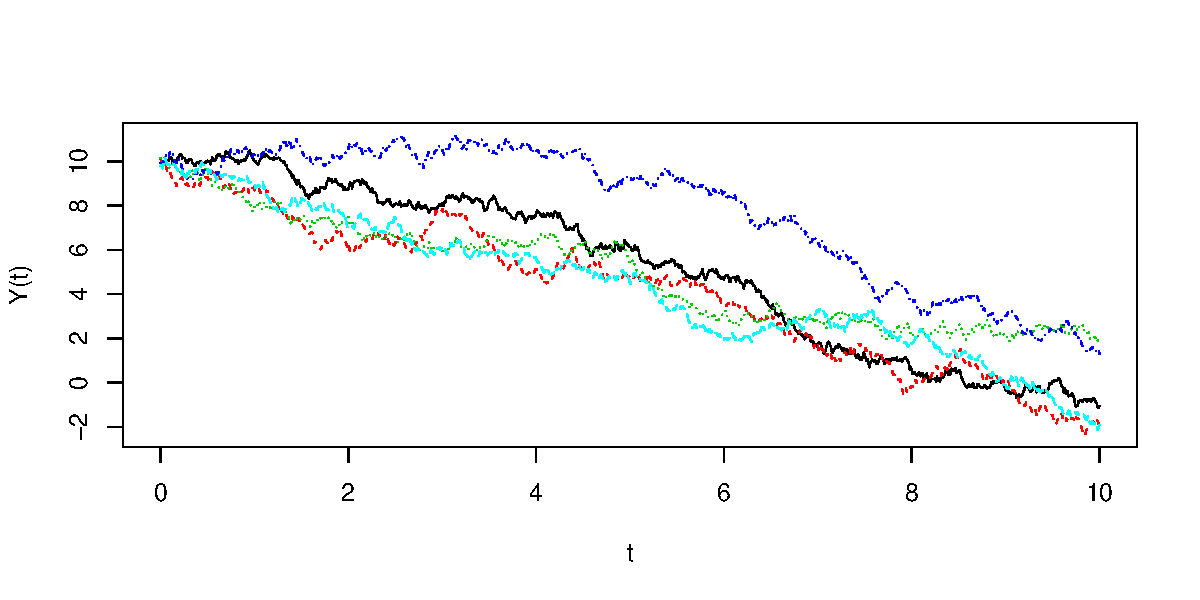
\includegraphics[scale=0.4]{figures/wiener_processes.pdf}
\end{figure}
\noindent{}Clearly, for a Wiener process starting in $y_0>0$ and with a downwards drift, i.e. $\mu>0$, the movement is markedly in the direction of zero. If $\sigma^2$ is small in comparison to the drift, as well as that the initial level is sufficiently high in comparison to $\sigma^2$, then the process will move in almost a straight line, such that
\begin{equation*}
    X(t)\approx y_0-\mu t.
\end{equation*}
Consequently, the first hitting time will be nearly a deterministic function of $y_0$ and $\mu$,
\begin{equation}
    T\approx \frac{y_0}{\mu}.
\end{equation}
This is quite visible in Figure \ref{plot:wiener}, which shows examples of 5 Wiener process paths with initial value $y_0=10$ and drift $\mu=1$. If $\sigma^2$ is relatively large compared to the drift, the diffusion part is more dominant and thus the hitting time is less predictable \citep{ABG}.

\subsection{Inverse Gaussian distribution and different parameterizations}
This parameterization is not in the exponential family, and hence it is not a generalized linear model.


\subsection{Wiener process and Inverse Gaussian first hitting time}
If we choose the stochastic process to be a Wiener process like in \eqref{wiener}, and we let the boundary be the non-positive numbers, $\setB=(-\infty,0]$, then \eqref{eq:fht-t} becomes
\begin{equation}
    T=\min_t\left(t\colon Y(t)\in\setB\right),
\end{equation}
i.e. the first hitting time is the time it takes for the process to first reach a non-positive value.
(Note that since the Wiener process is continuous, there is no difference between $\leq$ and $<$. We therefore use $<$ for convenience.)
It can be shown that the first hitting time of the Wiener process follows an inverse Gaussian distribution \citep{chhikara1988}, with probability distribution function (pdf)
\begin{equation}
\label{eq:ig-pdf}
    f(t|y_0,\mu,\sigma^2)=\frac{y_0}{\sqrt{2\pi\sigma^2t^3}}\exp\left[-\frac{(y_0+\mu t)^2}{2\sigma^2t}\right],
\end{equation}
and cumulative distribution function (cdf)
\begin{equation}
\label{eq:ig-cdf}
    F(t|\mu,\sigma^2,y_0)=\Phi\sqb*{-\frac{\mu t+y_0}{\sqrt{\sigma^2t}}}+\exp\p*{-\frac{2y_0\mu}{\sigma^2}}\Phi\sqb*{\frac{\mu t-y_0}{\sqrt{\sigma^2t}}}.
\end{equation}
As previously discussed in subsection \ref{fht-idea}, note that if the drift $\mu$ is positive, then it is not certain that the process will ever reach 0. Hence the probability distribution function in \eqref{eq:ig-pdf} is improper. In this case, the probability of the time not being finite is
\begin{equation}\label{eq:P-inf-FHT}
    \Pr{(T=\infty)}=1-\Pr{(T<\infty)}=1-\exp{(-2y_0\mu)},
\end{equation}
see \citet{cox1965}. Since we in survival analysis prefer working with the survival function $S(t)=1-F(t)$ rather than the cdf $F(t)$, we note that $S(t)$ becomes
\begin{equation}
\label{eq:ig-surv}
    S(t|\mu,\sigma^2,y_0)=\Phi\sqb*{\frac{\mu t+y_0}{\sqrt{\sigma^2t}}}-\exp\p*{-\frac{2y_0\mu}{\sigma^2}}\Phi\sqb*{\frac{\mu t-y_0}{\sqrt{\sigma^2t}}},
\end{equation}
where $\Phi(x)$ is the cumulative distribution function of the standard normal,
\begin{equation*}
    \Phi(x)=\int_{-\infty}^x\phi(y)\dy,
\end{equation*}
and $\phi(x)$ is the pdf of the standard normal, defined as
\begin{equation}
    \phi(x)=\frac{\exp\left(-x^2/2\right)}{\sqrt{2\pi}}.
\end{equation}
Note that in \eqref{eq:ig-surv} we used the fact that the cdf of the standard normal distribution is symmetric around 0,
meaning that we were able to swap
\begin{equation*}
    1-\Phi\sqb*{-\frac{\mu t+y_0}{\sqrt{\sigma^2t}}}
\end{equation*}
with
\begin{equation*}
    \Phi\sqb*{\frac{\mu t+y_0}{\sqrt{\sigma^2t}}}.
\end{equation*}

\subsection{The inverse gaussian is overdetermined if the health process is latent}
There are three parameters in the inverse Gaussian distribution, namely $y_0, \mu$ and $\sigma$.
We observe, however, that both the pdf $f(t|y_0,\mu,\sigma^2)$ in \eqref{eq:ig-pdf} and the survival function $S(t|\mu,\sigma^2,y_0)$ in \eqref{eq:ig-surv} only depend on these parameters through the ratios $\mu/\sigma$ and $y_0/\sigma$.
Hence, in reality there are only two free parameters.
In other words, we can without loss of generality fix one parameter.
The conventional way to proceed is to set $\sigma$ equal to 1 \citep{leewhitmore2006}, and in this thesis we follow the convention.

\section{Properties of the inverse Gaussian}

\subsection{The shape of the hazard function in the inverse Gaussian model}
From \eqref{eq:hfs}, we know that the hazard function can be seen as
\begin{equation*}
    \hz(t)=f(t)/S(t).
\end{equation*}
If we plug in the inverse Gaussian versions of $f(t)$ and $S(t)$, we would get a rather intractable expression.
However, we can make some comments on its shape as it relates to different values of $y_0$ and $\mu$.
If $y_0$ is close to zero, we essentially get a decreasing hazard rate.
If $y_0$ is far from zero, however, we essentially get an increasing hazard rate.
If $y_0$ is somewhat inbetween, we get a hazard rate which first increases and then decreases \citep{ABG}.
In all three cases, the hazard has a peak.
This peak is dependent on both the initial level and the drift, of course. 
It is not as simple as the peak being at the mean lifetime, i.e., $y_0/\mu$.
Although the height of the peak will change both by changing both parameters, to simplify it a lot, $y_0$ mostly impacts at what time the
peak is, whereas $\mu$ mostly affects the height of the peak.
Regardless of the initial value, the hazard rate converges to the same limiting hazard, which is
\begin{equation}
    \lim_{t\to\infty}\hz(t)=\frac{1}{2}\left(\frac{\mu}{\sigma}\right)^2=0.5\mu^2,
\end{equation}
as seen in \citet{ABG}. To get an intuitive feel for this, I have made an interactive website at \verb|vegarsti.shinyapps.io/FHT_Hazard|
\todo[inline]{Add plots and more explanation here.}
%\todo[inline]{Add plots of hazard rates here. see page 401 in ABG}

\subsection{Comparison of hazard rates}
It might be of particular interest to look at the ratio between two hazard rates. We might for example look at it when the drift $\mu$ is the same, but the initial level $y_0$ is different. Then the hazard ratio is strongly decreasing. This feature is the same phenomenon as that observed in frailty models, where the relative hazards often decline \citep{ABG}.
\todo[inline]{Add plot and explain better.}
It is also of interest to do the converse, that is, look at the hazard ratio when the initial level is the same, but the drift is different. The result here is quite different. The ratio of the hazards has a ``bathtub'' shape, which levels off at a later time \citep{ABG}. Keep in mind here that levelling off means getting to proportional hazards.
We see that the FHT framework with a Wiener process is a highly flexible parametric model for survival analysis. Indeed, much more flexible than Cox regression, since the hazard ratios in Cox are all confined to be constant over time.
\todo[inline]{Add plot here as well; also here see ABG page 402}

\section{Regression}\label{subsec:IG-reg}
We may introduce effects from covariates by allowing $\mu$ and $y_0$ to depend on covariates $\x$ and $\z$.
A simple and much used model \citep{leewhitmore2006, caroni2017} is to simply use the identity link function for the drift $\mu$, and to use the logarithm link function for the initial level $y_0$, since in our framework it must be positive:
\begin{equation}\label{eq:y0}
    \mu(\bbeta)=\bbeta^\T\x=\sum_{j=1}^p \beta_jx_j,
\end{equation}
\begin{equation}\label{eq:mu}
    y_0(\bgamma)=\exp(\bgamma^\T\z)\Rightarrow\ln y_0(\bgamma)=\bgamma^\T\z=\sum_{j=1}^d \gamma_jz_j.
\end{equation}
Here $\bbeta\in\R^p$ and $\bgamma\in\R^d$ are vectors of regression coefficients. Note that we may let $\x$ and $\z$ share none, some, or all elements. We will discuss consequences of this later.

Plugging in the pdf \eqref{eq:ig-pdf} and the survival function \eqref{eq:ig-surv} into the log-likelihood \eqref{eq:surv-lik}, we get that the log-likelihood of a survival data set with the inverse gaussian FHT model, is
\begin{align}\label{eq:loglik}
\begin{split}
    l(y_0,\mu,\sigma)=\sum_{i=1}^n&d_i\p*{\ln y_0-\frac{1}{2}\ln\p*{2\pi\sigma^2\ti^3}-\frac{\p*{y_0+\mu\ti}^2}{2\sigma^2\ti}} \\
    &+
    (1-d_i)\ln\p*{\Phi\p*{\frac{\mu\ti+y_0}{\sqrt{\sigma^2\ti}}}-\exp\p*{-\frac{2y_0\mu}{\sigma^2}}\Phi\p*{\frac{\mu\ti-y_0}{\sqrt{\sigma^2\ti}}}}.
\end{split}
\end{align}

\subsection{Fitting an IG FHT model}
At the moment, the standard for fitting an inverse gaussian FHT model to survival data is to use numerical likelihood maximization \citep{caroni2017}. A few software packages for doing this exist.For \verb|R| \citep{Rlang}, the \verb|threg| package \citep{threg}.
There does not exist any method to fit either a \textit{regularized} model at the moment, nor to do automatic variable selection.

%\todo[inline]{Add regression example}

%\subsection{Example of application}
%Lorem ipsum some example. Just use numerical maximization.

%\subsection{Identification problems}

\subsection{Combining clinical and genetic data in the Inverse Gaussian FHT model}
Combining clinical and genetic data in biomedical survival analysis is a large and important goal.
The IG FHT model lends itself nicely to combining clinical and genetic data.
As discussed in \citet{aalengjessing2001}, an a priori decision of splitting covariates as those relating to ``fixed'' covariates, e.g. genes, and covariates related to ``lifestyle,'' would be an instance of this combining of data.
With this perspective, it would be reasonable to let the initial health level $y_0$ be a function of the ``fixed'' covariates, while the drift would be a function of the ``lifestyle'' ones.
Furthermore, since genes are high-dimensional, this yields an easy way to combine high-dimensional data and low-dimensional data in the same model.
Other approaches used, e.g. related to Cox regression, require tuning and weighting of parameters.
\todo[inline]{more here}

    \chapter{Gradient boosting}\label{ch:boosting}
Boosting is one of the most promising methodological approaches for data analysis developed in the last two decades \citep{mayr14a}.
It has become a staple part of the statistical learning toolbox because it is a flexible tool for estimating interpretable statistical models.
Boosting, however, originated as a black box algorithm in the fields of computational learning theory and machine learning, not in statistics.

Computer scientists Michael Kearns and Leslie Valiant, who were working on computational learning theory, posed the following question \citep{kearnsvaliant}: 
Could any weak learner be transformed to become a strong learner?
A weak learner, sometimes also simple or base learner, is a learner that has a low performance.
For example, in the context of classification, a weak learner is one that performs only slightly better than random (uniform) chance.
In the binary classification setting, it would only perform slightly better than a coin flip.
Meanwhile, a strong learner should be able to perform in a near-perfect fashion, for example attaining high accuracy on a prediction task.
We will first give a summary of the history of boosting, starting with AdaBoost \citep{adaboost}, an algorithm that proved that the answer to the original question above was yes.
For a complete overview of the history of boosting, see \citet{mayr14a, mayr14b, mayr17}.

\section{AdaBoost: From machine learning to statistical boosting}
The original AdaBoost, also called Discrete AdaBoost \citep{adaboost} is an iterative algorithm for constructing a binary classifier $F(\cdot)$.
It was the first \textit{adaptive} boosting algorithm, as it automatically adjusted its parameters to the data based on its perfomance.
In the binary classification problem, we are given a set of observations
\begin{equation*}
    D=(\x_i,y_i)_{i=1}^N,
\end{equation*}
where $\x_i\in\R^p$ is a vector of covariates, and $y_i\in\{-1,1\}$ is a binary response, i.e., positive or negative; yes or no.
We want to find a rule which best separates these observations into the correct classes $\{-1,1\}$, as well as being able to classify new, unseen observations of the same form.
Some observations are hard to classify, whereas some are not.
\citet{adaboost} proposed that one could estimate several classifiers, and assign a weight $\alpha_m$ to each classifier.
By giving more weight to a more accurate classifier, a weighted sum of all of these classifications might be a good classification.
It turns out that this is the case.
We now give an explanation of the algorithm.

AdaBoost is an iterative algorithm.
In a given step $m$, we use a weak learner $h(\cdot)$ to estimate a classifier $\hat{h}^{[m]}(\cdot)$, that minimizes the weighted sum of misclassified points.
Based on the misclassification rate a weight $\alpha^{[m]}$ is assigned to the classifier $\hat{h}^{[m]}(\cdot)$.
After a first iteration, the classifier is $F_1(\cdot)=\hat{\alpha}^{[1]}\hat{h}^{[1]}(\cdot)$.
Using this initial classifier, some points will be correctly classified, and some will be misclassified.
We increase the weights of the misclassified ones, and normalize the weights afterwards, to ensure that the sum of the weights is always the same.
This results in the correctly classified observations having a reduced weight, and with misclassified observations having an increased weight.
In the following iteration, we apply again a weak learner which minimizes the weighted sum of the observations, and we reweight the observations accordingly, in the same manner as before.
Again, calculate a weight to give to this new classifier, and add it to the previous classifier, such that $F_2(\cdot)=\hat{\alpha}^{[1]}\hat{h}^{[1]}(\cdot)+\alpha^{[2]}h^{[2]}(\cdot)$.
Continue iterating in this fashion until an iteration number $\mstop$ is reached.
The resulting AdaBoost classifier $\hat{F}(\cdot)$ becomes
\begin{equation*}
    \hat{F}(\cdot)=F^{[\mstop]}(\cdot)=\sum_{m=1}^{\mstop}\hat{\alpha}^{[m]}\hat{h}^{[m]}(\cdot),
\end{equation*}
i.e. a linear combination of the weak classifiers, or in essence a weighted majority vote of weak learners given the observations.

The AdaBoost algorithm often carries out highly accurate prediction.
In practice, it is often used with stumps, which are decision trees with one split.
For example, \citet{bauer-kohavi} report an average 27\% relative improvement in the misclassification error for AdaBoost using stump trees, compared to the error attained with a single decision tree.
They conclude that boosting not only reduces the variance in the prediction error from using different training data sets, but that it is also able to reduce the average difference between the predicted and the true class, i.e., the bias.
\citet{breiman1998} supports this analysis.
Because of its plug-and-play nature and the fact that it never seemed to overfit, which occurs when the learned classifier degrades in test error because of being too specialized on its training set, Breiman remarked that ``boosting is the best off-the-shelf classifier in the world'' \citep{ESL}.

%Overfitting occurs when the out-of-sample error starts to increase. At this point, the model is starting to be too sensitive to the structure of the specific data set it is estimated on. One way of thinking about it is that it is starting to fit to the error terms. Since what we actually care about is the performance on a test set, we want to stop just before the model starts overfitting.
While originally developed for binary classification, boosting is now used to estimate the unknown quantities in more general statistical models and settings.
In the following we present boosting in a more general statistical regression scheme.
Moreover, In its original formulation the AdaBoost classifier does not have interpretable coefficients, and as such it is a so-called black-box algorithm.
This means that we are unable to infer anything about the effect of different covariates.
In statistics, however, we are interested in models which are interpretable.
In the rest of this chapter, we will discuss gradient boosting algorithms.
We will start by defining the problem such algorithms try to solve, and introduce some notation.
We will then explain the gradient descent algorithm, and, more precisely, gradient boosting.

%See some figure for a schematic overview of the algorithm.

\section{General model structure, setting, and chosen notation} %Statistical model fitting and setting
The aim of statistical boosting algorithms is to estimate and select the effects in structured additive regression models.
Consider a data set
\begin{equation*}
    D=\left(\x_i,\y_i\right)_{i=1}^N
\end{equation*}
containing the values of an outcome variable $\y$ and predictor variables $\x_1, \x_2,\ldots,\x_p$, forming covariate matrix $\X=(\x_1, \x_2,\ldots,\x_p)$.
We assume that the samples $i=1,\ldots,N$ are independently generated from an identical distribution over the joint space $\setX\times\setY$.
The input space of $\x$ is a possibly high-dimensional $\setX\in\R^p$ and the output space is a low-dimensional space $\setY$.
For the majority of applications, the output space $\setY$ is one-dimensional, but we will explicitly allow for multidimensional outcome variables.
Our objective is to model the relationship between $\y$ and $\x$ and to obtain an ``optimal'' prediction of $\y$ given $\x$.
To model the relationship, we will use an approach which very similar to the generalized additive model (GAM) approach \citep{gam-book}.
We will assume that the conditional outcome $\y|\x$ follows some probability distribution function (pdf)
\begin{equation}\label{eq:psi}
    \psi(\y|\theta(\x)),
\end{equation}
where $\theta$ is a parameter in the distribution function, typically related to the mean. We will at times refer to $\psi$ as a prediction function, when we use it to estimate parameters.
Further, we will model the distribution parameter $\theta$ as a functional of the covariates $\X$, with conditional expectation given the observed value $\x$ as
\begin{equation}
    g(\mathbb{E}(\theta(\x))=f(\x),
\end{equation}
where $g(\cdot)$ is a so-called link function and $f(\cdot)$ is a predictor.
We will discuss $f(\cdot)$ shortly.
We observe that if we use $g^{-1}(\cdot)$, i.e. the inverse of the link function, on this expression, we get
\begin{equation*}
    \mathbb{E}(\theta(\x))=g^{-1}(f(\x)).
\end{equation*}
This means that the conditional expectation of $\theta$ given the observed $\x$ is a transformation of the additive predictor $f(\x)$ using the inverse of the link function.
The link function will be chosen appropriately for the parameter $\theta$ in the distribution $\psi$, and is typically used to constrain the domain of the parameter.
For example, if we choose the logarithm as the link function, the inverse link function is the exponential function, meaning that
\begin{align}
    \mathbb{E}(\theta(\x))=\exp(f(\x)),
\end{align}
which will constrain the expectation to be a positive number.

The predictor $f(\cdot)$ can be modeled in many ways.
A common model is to let it be an \textit{additive} predictor, consisting of additive effects of single predictors.
This is called a generalized additive model (GAM), and it is specified by
\begin{equation}\label{eq:gam}
    f(\x)=\beta_0+f_1(x_1)+\ldots+f_p(x_p),
\end{equation}
where $\beta_0$ is a common intercept and the functions $f_j(x_j),j=1,\ldots,p$ are single predictors, which are partial effects of the variables $x_j$.
The generic notation
\begin{equation*}
    f_j(x_j)
\end{equation*}
may represent different types of predictor effects, such as classical linear effects $x_j\beta_j$, smooth non-linear effects constructed via regression splines, spatial effects or random effects of the explanatory variable $x_j$, and so on. 
%\todo[inline]{add citations on base learners here?}
The component-wise effects will typically be built up by additive estimation of base-learners, and statistical boosting is one way to perform this additive estimation.
Statistical boosting algorithms are one way to estimate such models.
These algorithms typically estimate $f(\x)$ by estimating component-wise effects for each component $j$, and these are in turn build up by estimation of base-learners $h_1(\cdot),\ldots,h_p(\cdot)$.
We will discuss this more in Section \ref{sec:component}, which introduces component-wise boosting.
\todo[inline]{See comments from Riccardo: Explain this better!}
We evaluate the fit of a model $\phi$ and its additive predictor $f(\cdot)$ by using a loss function $\rho(y,f(\cdot))$.
The loss function is a measure of the discrepancy between the observed outcome $\y$ and the additive predictor $f(\cdot)$.
In machine learning and optimization, one usually talks of loss functions, and as the name suggests, we wish to minimize the loss.
We will use the negative log-likelihood of the distribution of the response as a loss function because it is common in statistics \citep{mayr14a}.
In these cases, the loss function, which works on one set of observations $(\x_i,\y_i)$, is
\begin{equation*}
    \rho(\y_i,\theta(\x_i))=-\log{\psi(\y_i|\theta(\x_i))},
\end{equation*}
since the likelihood of one observation is simply the distribution given the observed data.
Note that there is a theoretical result stating that maximizing the log-likelihood is equivalent to minimizing the Kullback-Leibler Divergence, which is a measure of the difference between the distribution of the data itself and the assumed distribution $\psi$.
This shows that, having assumed a distribution $\psi$ for the responses, it is a good choice of loss function to use the log-likelihood of $\psi$.

\subsection{Example of a model and corresponding loss function}\label{subsec:model-example}
Let us consider at a specific example of a distribution and a loss function.
We have a dataset $D=(\x_i,y_i)_{i=1}^N$ where the responses $y_i$ are continuous and univariate.
We further assume that the responses follow a normal distribution, conditioned on the data.
Thus we wish to model the conditional mean $\mu(\x)$, and so we use $\mu$ instead of $\theta$.
Since the responses are continuous and normal, we do not need any transformation of the additive predictor, which means that the link function is the identity function,
\begin{equation*}
    g(\x)=\x.
\end{equation*}
Further, it means that
\begin{equation*}
    \mathbb{E}(\mu(\x))=f(\x).
\end{equation*}
For a normally distributed observation $y$, the likelihood is the familiar pdf,
\begin{equation*}
    f(y|\mu,\sigma^2)=\frac{1}{\sqrt{2\pi\sigma^2}}\exp\left\{-\frac{(y-\mu)^2}{2\sigma^2}\right\},
\end{equation*}
and we derive the loss function $\rho$ accordingly, yielding
\begin{align*}
    \rho(y,\mu(\x))&=-\log{f(y|\mu(\x))}\\
    &=\log{(\sqrt{2\pi\sigma^2})}+\frac{(y-\mu(\x))^2}{2\sigma^2} \\
    &\propto(y-\mu(\x))^2,
\end{align*}
which is the familiar $L_2$ loss function. Note that since we will only model $\mu(\cdot)$, the loss function need not depend on $\sigma^2$.
Similarly we have disregarded all proportionality constants.
With all those parts in place, we can model the additive predictor $f(\cdot)$.
One way to do this is by gradient boosting, which we will discuss soon.

\subsection{Model selection and model assessment}
Having chosen a distribution $\psi$ and a loss function $\rho$, we wish to find the parameter $\theta$ which minimizes the loss function of all unseen data
\begin{equation*}
    \left(\X,Y\right).
\end{equation*}
This means that we wish to minimize
\begin{equation}\label{eq:unseen-error}
    \Err(\theta)=\mathbb{E}_{Y,X}\left[\rho(Y,\theta(\X))\right].
\end{equation}
However, we are unable to estimate this quantity, as we do not have access to all such unseen data.
We therefore need a so-called \textit{test set}
\begin{equation*}
    D_{\text{test}}=\left(\x_i,\y_i\right)_{i=1}^{N_{\text{test}}}.
\end{equation*}
We can then calculate a test error $\Err$ of a specific $\theta$, which is the mean of the loss using $\theta$, over all observations in the test set $D_{\text{test}}$,
\begin{equation}\label{eq:test-error}
    \Err_{D_{\text{test}}}(\theta)=\frac{1}{N_{\text{test}}}\sum_{i=1}^{N_{\text{test}}} \rho(\y_i,\theta(\x_i)).
\end{equation}
$\Err_{D_{\text{test}}}$ is an estimate of $\Err$, since $D_{\text{test}}$ is a realization of unseen data.
To ensure that $\Err_{D_{\text{test}}}$ is an unbiased estimate, we will not use any data from the test set to estimate $\theta$.
To estimate $\theta$, we will therefore use a so-called \textit{training set}, which we will denote
\begin{equation*}
    D_{\text{train}}=\left(\x_i,\y_i\right)_{i=1}^{N_{\text{train}}}.
\end{equation*}
We can calculate the training error $\err(\theta)$, also called the \textit{in-sample error}, or the \textit{empirical risk}, which similarly is the sum of the loss function over all observations in the training set,
\begin{equation*}
    \err(\theta)=\frac{1}{N}\sum_{i=1}^{N} \rho(\y_i,\theta(\x_i)).
\end{equation*}
Our goal will be to use gradient boosting to minimize \ref{eq:test-error}.
To understand gradient boosting, we first need to understand the gradient descent algorithm.

\section{Gradient descent}
Suppose we are trying to minimize a differentiable multivariate function $G\colon\R^p\to\R$, where $p\in\N$.
Gradient descent is a so-called greedy algorithm for finding the minimum of such a function $G$, and one which is quite simple and surprisingly effective.
If all partial derivatives of $G$ at a point
\begin{equation*}
    \x^{[0]}=\left(x_1^{[0]},x_2^{[0]},\ldots,x_n^{[0]}\right)\in\R^p
\end{equation*}
exist, then the gradient of $G$ at $\x^{[0]}$ is the vector of all its partial derivatives at $\x^{[0]}$, namely
\begin{equation*}
    \nabla G\left(\x^{[0]}\right)=\left(\frac{\partial G(\x^{[0]})}{\partial x_1},\frac{\partial G(\x^{[0]})}{\partial x_2},\ldots,\frac{\partial G(\x^{[0]})}{\partial x_p}\right).
\end{equation*}
The motivation behind the gradient descent algorithm is that in a small interval around the point $\x_0$, $G$ is most decreasing in the direction of the negative gradient at that point.
Therefore, if we take a small step slightly in the direction of the negative gradient at $\x^{[0]}$, which we denote $\g^{[0]}$, from $\x^{[0]}$ to a new value $\x^{[1]}$, we end up with a slightly lower function value:
The new function value $G(\x^{[1]})$ will be smaller than $G(\x^{[0]})$.
The algorithm is greedy because it always goes in a direction which is immediately better.
The length $a^{[1]}$ of this small step is found by a line search, i.e., by finding the step length which gives the best $G(\x^{[1]})$, where then the new point is
\begin{equation*}
    \x^{[1]}=\x^{[0]}+a^{[1]}\cdot\boldsymbol{g}^{[0]}.
\end{equation*}
By repeating this procedure $\mstop$ number of times, the point $\x^{[\mstop]}$ will yield a minimum value of $G(\cdot)$.
The number of iterations $\mstop$ is decided by stopping when the decrease in function value is smaller than some pre-specified threshold $\epsilon>0$,
\begin{equation*}
    \mstop=\min_m G(\x^{[m-1]})-G(\x^{[m]})<\epsilon.
\end{equation*}
With sufficiently small steps, gradient descent will always converge, albeit possibly to a local minimum.
For a schematic overview of the algorithm, see Algorithm \ref{algo:grad-desc}.

\begin{algorithm}
\caption{Gradient descent}
\label{algo:grad-desc}
We wish to minimize $G(\x)$, i.e. solve $\min_{\x}G(\x)$, where $G$ is a multivariate function $G\colon\R^p\to\R$.
\begin{enumerate}
    \item
        Start with an initial guess $\x^{[0]}\in\R^p$, for example $\x^{[0]}=\0$, and set the number of iterations $m$ to 0.
    \item
        \label{grad-desc-iter}
        Increase the iteration number $m$ by 1.
    \item
        Calculate the direction to step in, i.e., the derivative at the current point,
        \begin{equation*}
            \g^{[m-1]}=-\nabla G(\x^{[m-1]}).
        \end{equation*}
    \item
        Solve the line search to find the best step length $a^{[m]}$,
        \begin{equation*}
            a^{[m]}=\argmin_{a}\x^{[m-1]}+a\cdot\g^{[m-1]}.
        \end{equation*}
    \item
        The step in iteration $m$ becomes
        \begin{equation*}
            \h_m=a^{[m]}\cdot\g^{[m-1]}.
        \end{equation*}
    \item
        Let $\x^{[m]}=\x^{[m-1]}+\h^{[m-1]}$.
    \item
        Decide if the algorithm should terminate by checking if the decrease in function value is smaller than the pre-specified threshold,
        \begin{equation*}
            G(\x^{[m-1]})-G(\x^{[m]})<\epsilon.
        \end{equation*}
        If this is true, set the number of iterations $\mstop$ to $m$, and go to the next step of the algorithm.
        If not, go to step \ref{grad-desc-iter}.
    \item
        The resulting minimum point for $G(\cdot)$ is
        \begin{equation*}
            \x^{[\mstop]}=\x^{[0]}+\sum_{m=1}^{\mstop}\h^{[m]}.
        \end{equation*}
\end{enumerate}
\end{algorithm}

The gradient descent algorithm is surprisingly robust.
Even though it may converge to a local minimum, it seems to often find good solutions globally.
This is likely related to research which has found that in high-dimensional spaces, most minima are not minima, but in fact, saddlepoints masquerading as local minima \citep{saddlepoints}.
This means that the size of the improvements in the function value $G(\cdot)$ will decrease since the gradient will be small at this saddlepoint.
When using a gradient descent method one typically sets a threshold $\epsilon$ at which the algorithm terminates when the gradient becomes smaller than the threshold, as we did.
However if the algorithm continues for a long enough time, then the multivariate gradient descent search should be able to continue to decrease the function value after it ``escapes'' the saddle point.



\section{The gradient boosting approach}
\subsection{Direct gradient descent on the loss function}
In a seminal paper, \citet{friedman2001} developed an iterative algorithm for fitting a predictor $f(\x)$, and he called the algorithm gradient boosting.
He showed that AdaBoost performs this algorithm for a particular loss function, namely the exponential loss function.
See \citet{ESL} for a good demonstration of Friedman's argument.
With his work, Friedman provided a way of viewing boosting through a statistical lens, and connected the successful machine learning approach to the world of statistical modelling.

The key idea of gradient boosting is to iteratively fit the different predictors with simple functions (base-learners) and combine the estimates into a predictor.
The base-learners are in particular fitted to the negative gradient of the loss function.

Consider data as in the example in subsection \ref{subsec:model-example}.
We have covariate vectors $\x_i$ and continuous responses $y_i$, where $i=1,2,\ldots,N$.
We assume that the conditional response $y_i$, given $\x_i$, follows a distribution $\psi(\theta)$ with a parameter $\theta$, which we will let depend on $\x_i$, i.e., $\theta(\x_i)$.
Based on the distribution $\psi$, we derive a loss function $\rho$, as seen in Subsection \ref{subsec:model-example}.
We wish to estimate the $\hat{\theta}(\cdot)$ that minimizes the training error, the empirical risk over the observed training data set
\begin{equation*}
    \argmin_{\hat{\theta}}\err(\theta)=\argmin_{\hat{\theta}}\frac{1}{N}\sum_{i=1}^{N} \rho(\y_i,\theta(\x_i)).
\end{equation*}
We can think of the empirical risk $\err(\theta)$ as a multivariate function $\err(\btheta)$, where the variables of the function are the parameter values of $\theta$ at each point $\x_i$,
\begin{equation*}
    \btheta(\x)=\left(\theta(\x_1),\,\theta(\x_2),\,\ldots,\,\theta(\x_N)\right).
\end{equation*}
These are plugged into the loss function for their corresponding observations, i.e.,
\begin{equation*}
    \err(\btheta(\x))=\err(\theta(\x_1),\,\theta(\x_2),\,\ldots,\,\theta(\x_N))=\frac{1}{N}\sum_{i=1}^{N} \rho(\y_i,\theta(\x_i)).
\end{equation*}
In this view, $\err$ is a multivariate function $\err\colon\R^N\to\R$.
We can therefore use gradient descent (see the previous section) directly on this function.
To do so, we consider $\hat{\theta}(\x_i)$ as a sum
\begin{equation*}
    \hat{\theta}(\x_i)=\beta_0+\sum_{m=1}^{m_{\text{stop}}}f^{[m]}(\x_i),
\end{equation*}
where the first term, $\beta_0$, is an initial guess which is common for all $\x_i$, and the remaining $\{\hat{f}^{[m]}(\x_i)\}_{m=1}^M$ function values are increments -- steps, or boosts.
%Note that this structure is the same as the decomposition of the solution to the gradient descent algorithm.
The initial guess $\beta_0$ should be the constant which minimizes the loss function $\rho$, e.g. the maxmimum likelihood constant in cases where the loss function is a negative log-likelihood.

To perform gradient descent on the $\err(\x_1,\,\x_2,\,\ldots,\,\x_N)$, we need to calculate its negative gradient.
The negative partial derivative for each observation is
\begin{equation*}
    -\frac{\partial}{\partial\theta(\x_i)} \rho(y_i,\theta(\x_i)).
\end{equation*}
Thus the gradient $\nabla \err(\btheta)$, which we will denote $\u$, and call generalized residuals, becomes
\begin{equation*}
    \u=\left(u_i\right)_{i=1}^N=\left(-\frac{\partial}{\partial \theta(\x_i)}\rho(y_i, \hat{\theta}(\x_i))\right)_{i=1}^N.
\end{equation*}
Since we now know how to calculate the gradient of a vector of estimated function values, we can constuct an algorithm for performing gradient descent on the loss function.
We initialize $\hat{\theta}^{[0]}(\x_i)$ to $\beta_0$ for all $\x_i$, where $\beta_0$ is found by
\begin{equation*}
    \beta_0=\argmin_{c}\err(c).
\end{equation*}
We then iterate.
In a step $m>0$, we calculate the negative gradient $\u^{[m-1]}$, and perform a gradient descent step in the direction $\u^{[m-1]}$.
The gradient descent step is
%As in the previous gradient descent algorithm, we 
\begin{equation*}
    \hat{\theta}^{[m]}(\x_i)=\hat{\theta}^{[m-1]}(\x_i)+a^{[m]}\cdot u_i^{[m-1]},
\end{equation*}
for each observation $\x_i$.
Thus in vector form, the step is
\begin{equation*}
    \hat{\btheta}^{[m]}(\x)=\hat{\btheta}^{[m-1]}(\x)+a^{[m]}\cdot \u^{[m-1]},
\end{equation*}
where the step length $a^{[m]}$ is found by a line search, as before.
After $\mstop$ number of steps, we will have converged to a solution $\hat{\btheta}^{[\mstop]}$,
\begin{equation*}
    \hat{\btheta}^{[\mstop]}=\hat{\theta}^{[\mstop]}(\x_1),\,\hat{\theta}^{[\mstop]}(\x_2),\,\ldots,\,\hat{\theta}^{[\mstop]}(\x_N),
\end{equation*}
which is a minimizer for the loss function $\err$.
This nonparametric approach would reduce the error of each data point.
However, it will not generalize to a similar data set where one observes different data points, since we only considers the points $\x_i$ in the training set.
We therefore need to do something else, and this is the functional gradient descent algorithm.


\subsection{Functional Gradient Boosting}\label{sec:FGD}
In the nonparametric approach from the previous subsection, we are only looking at the observed data points, and not at neighboring points in $\setX$ space.
We have to keep in mind that although we are optimizing the empirical risk over a specific data set, we are actually trying to minimize the expected value \eqref{eq:unseen-error}, i.e.,
\begin{equation*}
    \Err(\theta)=\mathbb{E}_{Y,X}\left[\rho(Y,\theta(\X))\right],
\end{equation*}
over all possible values of $\X$ and $Y$ in the joint distribution.
In addition, we wish to have an interpretable model.
Therefore, the we must impose smoothness to neighboring points in the $\setX$ space.
We can do this by choosing steps of (parameterized) \textit{functions} instead of steps of function \textit{values}, which is what we did in the previous subsection.
Therefore, since the solutions are parameterized functions, and we are performing gradient descent, the approach by \citet{friedman2001} develops a \textit{functional} gradient descent (FGD) algorithm, a gradient descent search in parameter space.
%In functional gradient descent, we still start with an initial value for $\hat{\theta}^{[0]}$, a constant $\beta_0$.
We now consider the estimate $\hat{\theta}$ to be a function which takes values in $\setX$,
\begin{equation*}
    \hat{\theta}(\x)=\beta_0+\sum_{m=1}^{\mstop}f^{[m]}(\x),
\end{equation*}
and it is composed of sums of an initial value $\beta_0$, and steps $\left\{f^{[m]}\right\}_{m=1}^{\mstop}$.
What is new is that now each $f^{[m]}(\x)$ is a parameterized function which we will estimate.
Since $f$ is now a parameterized function, we do not consider the training error $\err(\theta)$ to be a function of $N$ individual function parameter values $\theta(\x_i)$, $i=1,\ldots,N$, but rather just a function of $\theta$.
Hence, to derive the negative gradient of an estimate $\hat{\theta}$, i.e., we must differentiate the loss function $\rho$ with respect to $\theta$ instead of $\theta(x_i)$.
The generalized residuals, or the negative gradient, then become
\begin{equation*}
    \u=\left(-\frac{\partial}{\partial \theta}\rho(y_i, \hat{\theta}(x_i))\right)_{i=1}^N.
\end{equation*}
Then we iterate, let us say, at each step $m>0$ first calculating the generalized residuals of the previous iteration,
\begin{equation*}
    \u^{[m-1]}=\left(-\frac{\partial}{\partial \theta}\rho(y_i, \hat{\theta}^{[m-1]}(x_i))\right)_{i=1}^N,
\end{equation*}
like we have seen before.
Here we insert the model from the previous step, $\hat{\theta}^{[m-1]}$.
We now perform a gradient descent step.
However, we now constrain ourselves to steps which are functions of a base learner
\begin{equation*}
    \mathcal{H}(\cdot),
\end{equation*}
to ensure smoothness and generalizability, as discussed above.

A base learner is a class of functions $\mathcal{H}$ which is regularized, and often a simple effect of a parameter $\beta$.
Typical examples are linear least squares, stumps \citep[trees with one split, see][]{buhlmann2007,ESL}, and splines with a few degrees of freedom.
There are several reasons to use simple base learners in each step.
One is that there often exists fast methods for estimating a single base learner.
Therefore there will be little computational cost in each step. 
Secondly, there is more to gain by combining simple learners, rather than combining complex learners.
If we want to use complex learners, it is better to use another algorithm.

To take the steepest gradient in a functional sense, we must choose the realization of the base learner class $\mathcal{H}$ that produces the function $\hat{h}^{[m]}$ that is \textit{most parallel} to $\u^{[m-1]}$.
Another way of looking at it is that the best update is the member of the base learner function class $h$ that is most correlated with $\u^{[m-1]}$ over the data distribution.
This it means that $\hat{h}^{[m]}$ is the best approximation of the generalized residuals $\u^{[m-1]}$ by using $h(\cdot)$ to approximate with.
Equivalently, $\hat{h}^{[m]}$ is the projection of the generalized residuals onto the space spanned by the base learner function class.
We obtain $\hat{h}_m$ by fitting the base learner $\mathcal{H}$ to the generalized residuals.
The specific method of fitting will depend on the base learner.
If, for example, the base learner is a linear regressor, then the base learner will be
\begin{equation*}
    \hat{h}^{[m]}=\left(\hat{\bbeta}^{[m]}\right)^T\u^{[m-1]},
\end{equation*}
where the parameter is found by
\begin{equation*}
    \hat{\bbeta}^{[m]}=\left(\x ^T \x \right)^{-1}\x ^T \u^{[m-1]}
\end{equation*}
Having estimated the base learner, we do a line search to find the appropriate step length to use in order to minimize the loss function the most,
\begin{equation*}
    a^{[m]}=\argmin_{a}\err\left(\hat{\theta}^{[m-1]}+a\cdot\hat{h}^{[m]}{\cdot}\right).
\end{equation*}
We add the estimated learner times the step length to the current model, obtaining
\begin{equation*}
    \hat{\theta}^{[m]}(\cdot)\gets \hat{\theta}^{[m-1]}(\cdot)+a^{[m]}\hat{h}^{[m]}(\cdot).
\end{equation*}
We iterate this procedure until a stopping criterion is met.
The convention that has emerged is to specify a number of iterations $\mstop$.
This is the most important tuning parameter, and we will discuss it in the next subsection.
The resulting model
\begin{equation*}
    \hat{\theta}_{\text{FGD}}(\cdot)=\hat{\theta}^{[\mstop]}(\cdot)
\end{equation*}
has the additive structure that we discussed earlier, namely
\begin{equation*}
    \hat{\theta}(\x)=\beta_0+\sum_{m=1}^{\mstop}f^{[m]}(\x),
\end{equation*}
where each
\begin{equation*}
    f^{[m]}(\cdot)=a^{[m]}\cdot \hat{h}^{[m]}(\cdot).
\end{equation*}
This structure is a direct effect of the gradient descent algorithm, as the aggregation of base learners is strictly additive:
In every iteration, small increments are added to the additive predictor.
For a schematic overview of this algorithm, see Algorithm \ref{algo:fgd}.

The algorithm just described calculates error terms in each iteration, and performs functional gradient descent on them.
It is a very general framework, and it only requires a data set, a differentiable loss function, and a base learner.
It is therefore quite straightforward to derive specific algorithms to use for specific models:
It is just a matter of plugging in a chosen loss function and deriving its negative gradient.
This gives great flexibility.
We will now discuss the tuning parameters of the algorithm, which are very important to achieve good performance.

\begin{algorithm}
\caption{Gradient boosting, or, generic Functional Gradient Descent (FGD)}
\label{algo:fgd}
\begin{enumerate}
    \item
        Start with a data set $D=\{x_i, y_i\}_{i=1}^N$ and a chosen loss function $\rho(y,\theta(x))$, for which we wish to
        minimize the empirical risk, i.e., the loss function evaluated on the samples,
        \begin{equation*}
            \hat{\theta}=\argmin_{\theta}\err(\theta)=\argmin_{\theta}\sum_{i=1}^n\rho(y_{i},\theta(x_{i})).
        \end{equation*}
    \item
        Set iteration counter $m$ to 0.
        Initialize the additive predictor by setting $\hat{f}_0(\cdot)$ to a constant $\beta_0$.
        This constant should be the maximizer of the loss function,
        \begin{equation*}
            \beta_0(\cdot)=\argmin_c \err(c),
        \end{equation*}
        and it can be found e.g. through numerical maximization.
    \item
        Specify a base learner class $h$, e.g. linear least squares.
    \item
        \label{algo-fgd-step-inc}
        Increase $m$ by 1.
    \item
        Compute the generalized residuals (the negative gradient vector) of the previous iteration,
        \begin{equation*}
            \u^{[m-1]}=\left(-\frac{\partial}{\partial \theta}\rho(y_i, \hat{\theta}^{[m-1]}(x_i))\right)_{i=1}^N
        \end{equation*}
    \item
        Fit base learner $h$ to the generalized residuals $\u$ to obtain a fitted version $\hat{h}^{[m]}$.
    \item
        \label{algo-fgd-step-line}
        Find best step length for $a^{[m]}$ by a line search:
        \begin{equation*}
            a^{[m]}=\argmin_{a}\err\left(\hat{\theta}^{[m-1]}+a\cdot\hat{h}^{[m]}{\cdot}\right).
        \end{equation*}
    \item
        \label{algo-fgd-step-last-loop}
        Update the current estimated $\theta$,
        \begin{equation*}
            \hat{\theta}^{[m]}(\cdot)\gets \hat{\theta}^{[m-1]}(\cdot)+a^{[m]}\cdot \hat{h}^{[m]}(\cdot).
        \end{equation*}
    \item
        Repeat steps \ref{algo-fgd-step-inc} to \ref{algo-fgd-step-last-loop} (inclusive) until the iteration number $m$ is $\mstop$.
    \item
        Finally, return the estimated
        \begin{equation*}
            \hat{\theta}_{\text{FGD}}(\cdot)=\hat{\theta}^{[\mstop]}(\cdot)=\beta_0+\sum_{m=1}^{\mstop}a^{[m]}\hat{h}^{[m]}(\cdot).
        \end{equation*}
\end{enumerate}
\end{algorithm}

\subsection{Tuning parameters}
\subsubsection{Step length}
In the original generic functional gradient boosting algorithm, Algorithm \ref{algo:fgd}, the step length $a_m$ for each iteration is found through a line search, as in gradient descent.
\citet{friedman2001} says that fitting the data too closely may be counterproductive, and result in overfitting.
This has indeed proven to be true.
To avoid overfitting, we must constrain the fitting procedure.
This constraint is called regularization.
Friedman therefore proposes to regularize each step in the algorithm by a common learning rate, $\nu\in(0,1]$.
%It has often been found that regularization through shrinkage provides superior results \citep{copas1983}.
As we will see, most modern boosting algorithms omit the step of the line search entirely, i.e. step \ref{algo-fgd-step-line} in Algorithm \ref{algo:fgd}.
Instead, they fix a learning rate, or more commonly, step length $\nu$.
The choice of this step length is not of critical importance as long as it is sufficiently small \citep{schmid-hothorn}, i.e., it produces sufficient shrinkage, but the convention is to use $\nu=0.1$ \citep{mayr14a}.
This reduces the complexity of the algorithm, and it reduces the number of tuning parameters to the number of iterations $\mstop$ only.
There is a tradeoff between the number of iterations $\mstop$ and the size of the step length $\nu$.
If the step length is smaller, then a larger number of iterations is needed, and conversely, if the step length is large, a smaller number of iterations is needed.
We will now discuss the number of iterations.

\subsubsection{Number of iterations}\label{subsec:iterations}
With a fixed step length (learning rate), the main tuning parameter for gradient boosting is the number of iterations $\mstop$, i.e. the number of steps performed before the algorithm is stopped.
Its value is critical:
If $\mstop$ is too small, the model will underfit and it cannot fully incorporate the influence of the effects on the response and will consequently have poor performance.
On the other hand, too many iterations will result in overfitting, leading to poor generalization.
We know that we have either overfitting or underfitting if the estimated model $\hat{\theta}$ causes a high value of the test error $\Err(\hat{\theta})$.
It is easiest to notice overfitting if we calculate the test error as a function of the model complexity in.
In boosting, the model complexity increases with the number of steps.
The normal behaviour is that the test error will first decrease for a number of iterations, but then it will start to increase again.
The training error $\err$, on the other hand, will continue to decrease, so it is important to monitor by calculating test error.
The number of iterations is a very important tuning parameter.
We will discuss it more in-depth in Section \ref{sec:stop}.

%\subsection{Practical considerations}
%When boosting, one must (or should) center and scale the matrix $X$.

%\section{likelihood-based boosting}
%Lorem ipsum. \citep{DeBin2016} \citep{gamboost}.

\section{High dimensions and component-wise gradient boosting}\label{sec:component}
% add this to component-wise
\subsection{Problems in high dimensions}
In modern biomedical statistics, it is crucial to be able to handle high-dimensional data.
In some situations, a data set consists of more predictors $p$ than observations $N$.
When $p$ is much larger than $N$ ($p\gg N$), we talk about high-dimensional settings.
In order to address the issue of analyzing high-dimensional data sets, a variety of regression techniques have been developed over the past years.
Many of these techniques are characterized by a built-in mechanism for regularization.
One such technique, which can cope with the $p\gg N$ situation, is a version of boosting called component-wise boosting.

%\subsection{Regularization}
%In methods with built-in regularization, shrinkage of coefficient estimates or selection of relevant predictors is carried out \textit{simultaneously} with the estimation of the model parameters.
%Both shrinkage and variable selection will typically improve prediction accuracy:
%In case of shrinkage, estimators tend to have a slightly increased bias but a decreased variance, while in case of variable selection, overfitting the data is avoided by selecting only the most informative predictors.
%For instance if we are to use a least squares base learner which uses all $p$ dimensions, we see that it is infeasible:
%The matrix which must be inverted is singular when the number of predictors $p$ is larger than the number of observations $N$.
%For other models, it might be possible to estimate parameters for each predictor, but it would very easily result in overfitting.
%This is due to the ``curse of dimensionality,'' which states that in high-dimensional space, virtually all points are very far apart.
%Since the points are far apart, there are a vast number of ways that the variation can be explained, and very few of these will capture a generalized structure.
%Similarly, for variable selection, typical regimes such as \textit{forward stepwise variable selection} are infeasible to carry out, because it requires refitting all covariates in each new step, and it might be necessary to carry out a lot of steps.
%It is also clearly impossible to perform an exhaustive search of all combinations, as the number of models will suffer from the combinatorial explosion, i.e. that the number of models increases incredibly fast as the number of predictors $p$ increases.
%Note that regularization is not only useful in the high-dimensional data setting, but also tends to improve prediction accuracy in low-dimensional settings where $p\leq N$.

\subsection{The component-wise boosting approach}
The key idea of the component-wise approach to gradient boosting is to add the effect of only one variable at a time, instead of adding a small effect from all variables, as is the case in the generic FGD algorithm (Algorithm \ref{algo:fgd}).
Component-wise gradient boosting is an algorithm which works very well in these settings.
In fact, Buhlmann believes that it is mainly in the case of high-dimensional predictors that boosting has a substantial advantage over classical approaches \citep{buhlmann2006}.
The component-wise approach was first proposed in \citep{buhlmann-yu}, and component-wise boosting is a very active field of research \citep{buhlmann2006, mayr14a, mayr14b, mayr17}.
Consider yet again the case where we have a data set $D=(\x_i,y_i)_{i=1}^N$, where $\x_i\in\R^p$ are covariate vectors of a high dimension $p$, and $N$ is the number of observations.
Specifically, we are in a setting where $p>N$.
We want to finding the parameter $\theta$ which minimizes the empirical risk of a chosen loss function $\rho$ on the data set,
\begin{equation*}
    \hat{\theta}=\argmin_{\theta}\err(\theta)=\argmin_{\theta}\sum_{i=1}^n\rho(\y_i,\theta(\x_i)),
\end{equation*}
where the parameter $\theta$ is a predictor $\theta\colon\R^p\to\R$.
However, we will now let $\theta$ be an additive predictor, meaning it is a sum of partial effects of covariates,
\begin{equation*}
    \theta(\x)=\beta_0+\sum_{j=1}^p f_j(x_j).
\end{equation*}
These partial effects of the covariates will be estimated by component-wise learners in an iterative fashion.

\subsection{The component-wise boosting algorithm}
The structure of the component-wise boosting algorithm is very much the same as the generic functional gradient boosting algorithm (Algorithm \ref{algo:fgd}), but with some additional steps.
As mentioned, instead of using a base learner which incorporates all predictors, we use a set $\mathcal{H}$ of base learners consisting of a separate base learner for each component of the covariates.
The learners typically share the same structure, i.e., they are the same base learner, applied to different covariates.
For example, if we use a linear least squares model as base learners, the set of base learners would be
\begin{equation*}
    \mathcal{H}=\{h_1(\x;\beta_j)\}_{j=1}^p=\{\beta_j x_j\}_{j=1}^p
\end{equation*}
It is not necessarily the case that the learners have the same structure, it is also possible to include e.g. spline learners for some components, and least squares for others.
However, in the following, we will assume that each component only has one base learner, and that it is the same structure, which simplifies our notation a bit.

The initialization of the algorithm is the same as in the FGD algorithm:
We first initialize the additive predictor $\hat{\theta}^{[0]}$ to a constant $\beta_0$.
We then iterate.
In a given iteration $m$, we first construct the generalized residuals, by calculating the negative gradient.
Here we insert the additive predictor from the previous step, namely $\hat{\theta}^{[m-1]}$,
\begin{equation*}
    \u^{[m-1]}=\left(-\frac{\partial}{\partial \theta}\rho(y_i, \hat{\theta}(\x_i)\right)_{i=1}^N.
\end{equation*}
Note that this calculation is exactly like in the generic gradient boosting algorithm.
While the generic FGD algorithm here only estimated a single base learner, in the component-wise we estimate all base learners separately.
We obtain $p$ estimated functions
\begin{equation*}
    \hat{h}_1^{[m]}(\cdot),\,\hat{h}_2^{[m]}(\cdot),\,\ldots,\,\hat{h}_p^{[m]}(\cdot).
\end{equation*}
These estimated functions can again be viewed as approximations of the negative gradient vector, or equivalently the projection of the negative gradient vector onto the space spanned by the component-wise base learner.
However, these are projections onto only one dimension of the covariate space.
We wish to reduce the error $\err$ as much as possible, and so we select the covariate which has a corresponding estimated base learner which explains as much as possible of the variation in $\u^{[m-1]}$.
To select the best-fitting base-learner, we select the one with the smallest residual sum of squares error
\begin{equation*}
    j^{[m]}=\argmin_{j\in\{1,2,\ldots,p\}}\sum_{i=1}^N \left(u_i-\hat{h}_j^{[m]}\right)^2.
\end{equation*}
Note that this makes sense from a linear algebra perspective:
Choosing the one with minimal RSS means that we choose the one with the smallest projection error, or the one with the most signal.
We add this best-fitting base-learner $h_{j^{[m]}}^{[m]}$ to the current model, with a pre-specified step length of $\nu$, again typically set to 0.1, for the purpose of regularization.
Hence the model after iteration $m$ is
\begin{equation*}
    \hat{\theta}^{[m]}(\cdot)\gets \hat{\theta}^{[m-1]}(\cdot)+\nu\cdot\hat{h}^{[m]}_{j^{[m]}}.
\end{equation*}
Seen from a component-wise perspective, we update the predictor of the selected component,
\begin{equation*}
    \hat{f}_{j^{[m]}}^{[m]}(\cdot)\gets \hat{f}_{j^{[m]}}^{[m-1]}(\cdot)+\nu\cdot\hat{h}^{[m]}_{j^{[m]}},
\end{equation*}
\todo[inline]{This should be better!}
and for all other components $j\in\{j\colon j\neq j^{[m]},\,j=1,2,\ldots,p\}$, the update in iteration $m$ is simply
to keep the predictor from the last iteration
\begin{equation*}
    \hat{f}_{j}^{[m]}(\cdot)\gets \hat{f}_{j}^{[m-1]}.
\end{equation*}
We continue iterating until the iteration number $m$ reaches the pre-specified stopping iteration $m_{\text{stop}}$.
We will discuss selection of $\mstop$ in Section \ref{sec:stop}.
The final additive predictor becomes
\begin{equation*}
    \hat{\theta}=\hat{\theta}^{[m_{\text{stop}}]}=\beta_0 + \sum_{m=1}^{m_{\text{stop}}}\nu\cdot\hat{h}_{j^{[m]}}^{[m]}(\cdot).
\end{equation*}
Note that any base-learner $h_j$ can be selected at multiple iterations.
The partial effect of the variable $x_j$ is the sum of the estimated corresponding base learner in all iterations where it was selected.
Hence each $\hat{\theta}_j^{[\mstop]}(x_j)$ can be seen as
i.e.,
\begin{equation*}
    \hat{\theta}_j(x_j)=\sum_{m=1}^{m_{\text{stop}}}\nu\cdot\hat{h}_j^{[m]}(x_j)\indicator\left(j^{[m]}=j\right),
\end{equation*}
where $\indicator(\cdot)$ is an indicator function.
Hence the resulting additive predictor is a sum of component-wise predictors in the GAM form of
\begin{equation*}
    \hat{\eta}(\x)=\beta_0+\sum_{j=1}^p \hat{f}_j(x_j).
\end{equation*}
For a schematic overview of the algorithm, see Algorithm \ref{algo:component-wise}.
This algorithm has been implemented in R as \verb|mboost| \citep{mboost, mboost1, mboost2}, and it contains many different base learners which can be included in the model.

\begin{algorithm}
\caption{Component-wise gradient boosting}\label{algo:component-wise}
\begin{enumerate}
    \item
        Start with a data set $D=\{x_i, y_i\}_{i=1}^N$ and a chosen loss function $\rho(y,\theta(x))$, for which we wish to
        minimize the empirical risk, i.e., the loss function evaluated on the samples,
        \begin{equation*}
            \hat{\theta}=\argmin_{\theta}\err(\theta)=\argmin_{\theta}\frac{1}{N}\sum_{i=1}^N\rho(y_i,\theta(x_i)).
        \end{equation*}
    \item
        Set iteration counter $m$ to 0.
        Specify a step length $\nu$.
        Initialize the additive predictor by setting $\hat{f}_0(\cdot)$ to a constant $\beta_0$.
        This constant should be the maximizer of the loss function,
        \begin{equation*}
            \beta_0(\cdot)=\argmin_c \err(c),
        \end{equation*}
        and it can be found e.g. through numerical maximization.
    \item
        Specify a set of base learners $\mathcal{H}=\{h_1(\cdot),\dotsc,h_p(\cdot)\}$, where each $h_j$ is univariate and takes column $j$ of $\X$.
    \item
        \label{first-step}
        Increase $m$ by 1.
    \item
        Compute the negative gradient vector, i.e., the generalized residuals after the previous iteration of the boosted model,
        \begin{equation*}
            \u^{[m-1]}=\left(-\frac{\partial}{\partial \theta}\rho(y_i, \hat{\theta}(x_i))\right)_{i=1}^N.
        \end{equation*}
    \item
        For each base learner $h_j\in\mathcal{H},j=1,\ldots,p$, estimate $\hat{h}_{j}^{[m]}$ by fitting $(\x_i,u_i)_{i=1}^N$ using the base learner $h_j(\cdot)$.
        We obtain
        \begin{equation*}
            \hat{h}_1^{[m]}(\cdot),\hat{h}_2^{[m]}(\cdot),\ldots,\hat{h}_p^{[m]}(\cdot).
        \end{equation*}
    \item
        Select the best-fitting component $j^{[m]}$, i.e., with lowest RSS,
        \begin{equation*}
            j^{[m]}=\argmin_{j\in\{1,2,\ldots,p\}}\sum_{i=1}^N \left(u_i-\hat{h}_j^{[m]}\right)^2.
        \end{equation*}
    \item
        \label{last-step}
        Update the current model with the best-fitting model from the current iteration
        \begin{equation*}
            \hat{\theta}^{[m]}(\cdot)\gets \hat{\theta}^{[m-1]}(\cdot)+\nu\cdot \hat{h}_{j^{[m]}}^{[m]}(\cdot).
        \end{equation*}
    \item
        Repeat steps \ref{first-step} to \ref{last-step} (inclusive) until the iteration number $m$ is $m_{\text{stop}}$.
    \item
        Return the final boosted additive predictor
        \begin{equation*}
            \hat{\theta}(\cdot)=\hat{\theta}^{[m_{\text{stop}}]}(\cdot)=\beta_0+\sum_{m=1}^{m_{\text{stop}}}\nu\cdot\hat{h}_{j^{[m]}}^{[m]}(\cdot)
        \end{equation*}
\end{enumerate}
\end{algorithm}

\subsection{Component-wise boosting performs data-driven variable selection}
\label{sec:variable-selection}
Stopping the algorithm before every base-learner was at least selected once effectively excludes all non-selected base-learners, and thus also the corresponding covariates, from the final model.
The algorithm is therefore able to perform variable selection and model fitting simultaneously.
Furthermore, early stopping shrinks effect estimates toward zero \citep{buhlmann2007, DeBin2016}, similar to $L_1$-penalized regression
such as the lasso \citep{lasso, efron2004}.
Shrinkage of effect estimates lead to a lower variance and therefore to more stable and accurate predictions \citep{efron1975, copas1983, ESL}.


In other words, if the number of iterations $\mstop$ is small enough, the component-wise gradient boosting algorithm will carry out automatic variable selection.
In particular the base learners applied to irrelevant variables will never be considered in the updating step, and therefore many of the covariates in $\x$ will not be a part of the final model.
Some predictors will have more explanatory power, or signal, than others, and so they will be selected more often.
This is because some predictors are more correlated with the output than others.

%\citep{mayr-hofner}.

\section{Selecting the iteration number $\mstop$}
\label{sec:stop}
As we have mentioned in subsection \ref{subsec:iterations}, the crucial tuning parameter in boosting is the number of iterations, $\mstop$. 
Stopping a boosting procedure early enough will lead to variable selection and shrinks the parameter estimates toward zero.
In the case of $p<N$, with $m\to\infty$, the parameters in boosting will converge towards the maximum likelihood estimates \citep{DeBin2016}, i.e., minimizing the in-sample error.
We are, on the other hand, interested in minimizing the test error $\Err(\theta)$ with respect to $\theta$.
When using a gradient boosting algorithm, we do so on a data set $D$.
We choose an appropriate loss function, we specify base learners, and we specify a learning rate.
When these four factors are fixed, the parameter path will be deterministic.
This means that running the boosting algorithm the same number of steps $m$ several times will lead to the same $\hat{\theta}^{[m]}$.
There is no randomness in the estimates.
This is quite obvious if we think about it, because at any given step, the algorithm selects the component and learner which leads to the best decrease in training error, and there is nothing random in that.
The point of this is that we can view the test error of an estimated boosting model $\hat{\theta}^{[m]}$ as a function of the number of iterations used to produce it, i.e.,
\begin{equation}\label{test-error-m}
    \Err(m)=\Err(\hat{\theta}^{[m]}).
\end{equation}
There exists an $m$ which minimizes $\Err(m)$.
Many authors state that the algorithm should be stopped early, but do not go further into the details.
What we want is therefore a good method for approximating $\Err(m)$.
This can be done in a number of ways.
Common model selection criteria such as the Akaike Information Criteria (AIC) may be used, however the AIC is dependent on estimates of the model's degrees of freedom. 
Initial versions of boosting used it, but practice showed that AIC-based stopping rules lead to overfitting \citep{mayr-hofner}.
For $\text{L}_2\text{Boost}$, \citet{buhlmann2007} suggest that $\df(m)=\trace(B_m)$ is a good approximation.
Here $B_m$ is the hat matrix resulting from the boosting algorithm.
This was, however, shown by \citet{hastie2007} to always underestimate the actual degrees of freedom.
\citet{mayr-hofner} propose a sequential stopping rule using subsampling.
However this is computationally very expensive and not really used in practice.
None of these rules, in other words, are optimal to use.
Instead, cross-validation, a general and very common method for selection of tuning parameters in statistics, is what is used in almost all cases \citep{mayr14a,mayr14b,mayr17}.
Cross-validation is flexible and easy to implement.
It is somewhat computationally demanding, because it requires several full runs of the boosting algorithm, but it is otherwise quite simple.
We now give an explanation of this procedure.

%\subsection{Other selection methods}
%The number of iterations in the boosting procedure, $M$, is a tuning parameter. It acts as a regularizer. AIC, etc.

\subsection{K-fold cross-validation}\label{subsec:K-fold}
K-fold cross-validation \citep{lachenbruch}, or simply cross-validation, is a general method for estimating the test error and therefore commonly used for selection of penalty or tuning parameters.
In cross-validation, the data are randomly split into K rougly equally sized folds.
For a given fold $k$, all folds except $k$ act as the training data and used to estimate the model.
The resulting model is then evaluated on the unseen data, namely the observations belonging to fold $k$.
This procedure is repeated for all $k=1,\ldots,K$.
An estimate of the test error is obtained by averaging over the test errors evaluated in each left-out fold.
Let $\kappa(k)$ be the set of indices for fold $k$.
The cross-validated estimate for a given $m$ then becomes
\begin{equation*}
    \CV(m)=\frac{1}{K}\sum_{k=1}^K\sum_{i\in\kappa(k)}\rho(y_i,\hat{y}_i^{-\kappa(k)}).
\end{equation*}
$\CV(m)$ is an estimate of the test error of gradient boosting as a function of the iteration number $m$ \eqref{test-error-m}.
For each iteration $m$, we calculate the estimate of the cross-validated prediction error $\CV(m)$.
We choose $\mstop$ to be the minimizer of this error,
\begin{equation*}
    \mstop=\argmin_{m}\CV(m).
\end{equation*}
Typical values for $K$ are 5 or 10, but in theory one can choose any number. The extreme case is $K=N$, called leave-one-out cross-validation, where all but one observation is used for training and the model is evaluated on the observation that was left out. In this case, the outcome is deterministic, since there is no randomness when dividing into folds.

\subsection{Stratified cross-validation}
When dividing an already small number of survival data observations into $K$ folds, we might risk getting folds without any observed deaths, or in any case, very few. In stratified cross validation, we do not divide the folds entirely at random, but rather, try to divide the data such that there is an equal amount of uncensored data in each fold.
As before, let $\kappa(k)$ be the set of indices for fold $k$.
Divide the observed data into $K$ folds, as with usual cross validation, to get an index set $\kappa_{\delta=1}(k)$ for a given $k$. 
Similarly, divide the censored data into $K$ folds, obtaining $\kappa_{\delta=0}(k)$.
Finally, $\kappa(k)$ is the union of these sets: $\kappa(k)=\kappa_{\delta=1}(k)\cup\kappa_{\delta=0}(k)$.
For a detailed description of 10-fold cross-validation issues in the presence of censored data, see \citet{kohavi}.

\subsection{Repeated cross-validation}\label{subsec:repeated-cv}
The randomness inherent in the cross-validation splits has an effect on the resulting $\mstop$.
This is true in general, but it is especially true for real-life survival data, because such data sets typically have small effective sample sizes (number of observed events).
We can easily imagine that we can end up with quite different values for $\mstop$ for two different splits of the data, depending on which folds the events end up in.
It has been very effectively demonstrated that the split of the folds has a large impact on the choice of $\mstop$ \citep{seibold}.
To reduce the impact of this issue, \citet{seibold} suggest to repeat the cross-validation scheme a few times and average the results.
They show that repeating the cross-validation procedure even only 5 times effectively averages out the randomness.
In other words, we divide the data into $K$ folds, and repeat this $J$ times.
Now let $\kappa(j, k)$ be the $k$-th fold in the $j$-th split.
We end up with a new estimate for the prediction error,
\begin{equation*}
    \RCV(m)=\frac{1}{J}\sum_{j=1}^J\frac{1}{K}\sum_{k=1}^K\sum_{i\in\kappa(j,k)}\rho(y_i,\hat{y}_i^{-\kappa(j,k)}).
\end{equation*}
Again, $\RCV(m)$ is also an estimate of \eqref{test-error-m}, but with less variance due to averaging several results.
As before, we choose $\mstop$ to be the minimizer of this error,
\begin{equation*}
    \mstop=\argmin_{m}\RCV(m).
\end{equation*}
To carry out this in practice when using a boosting algorithm, we let the boosting algorithm run for $m=1$ to $m=M$, where $M$ is a large number that we are sure will result in a overfitted model.
Thus we ensure that we find the minimizing $m$, and not a local minimum.

\section{Multidimensional boosting}
A limitation of the boosting methods we have described so far, as well as of $L_1$-penalized estimation such as the lasso method \citep{lasso}, is that they are designed for statistical problems involving a one-dimensional prediction function.
By only considering such functions, we are restricted to estimating models which only model a single quantity of interest, which is almost always the mean.
In many applications, modelling only one parameter will not be sufficient \citep{kneib2013}.
We want to be able to estimate more general models, in which more quantities, e.g. the drift and the threshold of the models described in section \ref{sec:FHT}, can be explained by covariates.
To properly estimate such an FHT model, we therefore need a more general gradient boosting algorithm which is able to estimate several parameters.
Typical examples of multidimensional estimation problems are classification with multiple outcome categories and regression models for count data.
Another example is estimating models in the GAMLSS family \citep{gamlss}.
GAMLSS, which refer to ``generalized additive models for location, scale and shape,'' are a family of models that relates not only the mean, but all parameters of the outcome distribution to the available covariates.
GAMLSS are in this sense an extension of GAM models \citep{gam-book}.
A gradient boosting algorithm called \textit{gamboostLSS} was developed for boosting such models \citep{gamboostlss-paper}.
The algorithm framework used in \textit{gamboostLSS} is inspired by the multidimensional boosting algorithm first introduced in \citet{schmid}.
We will here explain the \textit{gamboostLSS} algorithm, as presented in \citet{gamboostlss-paper}.

There are two versions of the multidimensional gradient boosting algorithm.
One, which originated first, is now referred to as cyclical, and the other is the noncyclical version.
%We will now give a brief summary of these two.
In the cyclical version, each parameter dimension is updated with a component-wise learner.
In the noncyclical version, only one parameter dimension is updated, specifically the parameter dimension update that leads to the best decrease in training error (log-likelihood).
The cyclical version is somewhat more stable in the variable selection, but it requires a vector of stopping iterations $\boldsymbol{m_{\text{stop}}}$, to be found by grid search \citep{thomas2018}.
Thus, it is much faster to use the noncyclical version.

\section{Cyclical \textit{gamboostLSS}}\label{sec:gamlssboost}
A key feature of the GAMLSS model family is that every parameter of the conditional response distribution is modelled by its own predictor and associated link function.
Traditional GAMs \citep{gam-book} are typically restricted to modelling the conditional mean of the response variable, and treats possible other distributional parameters as fixed.
GAMLSS, on the other hand, allows for regression of each distribution parameter on the covariates.
Common distribution parameters are location, scale, skewness and kurtosis, but degrees of freedom (of a $t$-distribution) and zero inflation probabilities can be modelled as well \citep{gamboostlss-paper, gamboostLSS-manual}.
Thus, in the GAMLSS approach, the full conditional distribution of a multiparameter model is related to a set of predictor variables of interest.
Similarly to in GAMs, in GAMLSS the structure of each predictor is assumed to be additive.
Hence a wide variety of functional predictors can be included in each predictor.
Examples include non-parametric terms based on penalized splines, varying-coefficient terms and spatial and subject-specific terms for repeated measurements.
The estimation of GAMLSS coefficients is usually based on penalized likelihood maximization; for details on fitting procedures, see \citet{gamlss}.

\subsection{GAMLSS}\label{subsec:GAMLSS}
The GAMLSS model class assumes observations $y_i$ for $i=1,2,\ldots,N$ that are conditonally independent given a set of covariates and after having accounted for spatiotemporal effects.
The conditional density
\begin{equation}\label{gamlss-density}
    \psi(y_i|\btheta(x_i)),
\end{equation}
may depend on $K$ distribution parameters
\begin{equation*}
    \btheta_i=\left(\theta_{i,1},\theta_{i,2},\ldots,\theta_{i,K}\right)^T.
\end{equation*}
Each distribution parameter $\theta_k,k=1,2,\ldots,K$ is modelled by its own additive predictor $\eta_{k}$ and depends additively
on the covariates.
$\theta_k$ is linked to its predictor by a known monotonic link function
\begin{equation*}
    g_k(\cdot).
\end{equation*}
Letting $p_k$ be the number of covariates to be used for distribution parameter $\theta_k$,
\begin{equation*}
    x_{k,1},x_{k,2},\ldots,x_{k,p_k}
\end{equation*}
are the covariates in the model of the parameter $\theta_k$.
A GAMLSS is given by the equations
\begin{equation*}
    \eta_k\coloneqq g_k(\theta_k)=\beta_{k,0}+\sum_{j=1}^{p_k}f_{k,j}(x_{k,j}),
\end{equation*}
for all $k=1,2,\ldots,K$. Here $\beta_{k,0}$ is the intercept for distribution parameter $\theta_k$, and $f_{k,j}$ represents the type of effect that covariate $j$ has on the distribution parameter $\theta_k$, through the link function.
In the case of a simple linear regression learner, a component-wise effect of component $j$ on distribution parameter $\theta_k$ would be
\begin{equation*}
    f_{k,j}(x_{k,j})=x_{k,j}\beta_{k,j},
\end{equation*}
where $\beta_{k,j}$ is a parameter to be estimated.
Finally, $\eta_{k}$ is the additive predictor for $\theta_k$.
Note that a GAMLSS reduces to a GAM \citep{gam-book} in the case where the distribution parameter vector is a scalar
\begin{equation*}
    \btheta_i=\theta_i=\mu_i,
\end{equation*}
i.e., the conditional mean of observation $i$.
For parametric models, the unknown quantities of a GAMLSS can be estimated by maximizing the log-likelihood of an observed data set of $N$ observations of the conditional density \eqref{gamlss-density}.
The log-likelihood contribution for one sample is
\begin{equation*}
    \log\{\psi(\btheta(x_i)|y_i)\},
\end{equation*}
$\hat{\theta}$ will be a functional which works on the covariate vector $\x$.
Hence the total log-likelihood is
\begin{equation*}
    l(\btheta)=\sum_{i=1}^N\log\left(\psi(\btheta(x_i)|y_i)\right),
\end{equation*}
Denoting estimates of the prediction functions as $\hat{\eta}_k$, estimates of the distribution parameters $\btheta$ are then obtained from transforming back via the inverse link functions,
\begin{equation*}
    \hat{\theta}_k=g_k^{-1}(\hat{\eta}_{\theta_k}),
\end{equation*}
for all $k=1,2,\ldots,K$, i.e., $\hat{\btheta}=\left(\theta_1,\theta_2,\ldots,\theta_K\right)$ is an estimate of $\btheta$.
After the original GAMLSS paper \citep{gamlss}, a penalized likelihood approach based on modified versions of the backfitting algorithm for GAM estimation was developed by the same authors \citep{gamlssR}.
Later, however, a gradient boosting algorithm, called \textit{gamboostLSS}, was developed \citep{gamboostlss-paper}.
The algorithm \textit{gamboostLSS} uses a strategy for multidimensional boosting proposed by \citet{schmid}.
\citet{thomas2018} later coined the term ``cyclical'' to describe it and here we use this notation.

\subsection{The \textit{gamboostLSS} algorithm}
The main idea of the cyclical multidimensional boosting algorithm is to have a boosting step for each parameter $k$ in each iteration, and to successively update the predictors in each iteration.
We cycle through all parameter dimensions in each boosting iteration.
In every dimension $k$, we carry out one boosting iteration.
This boosting iteration can in principle be the same as in the generic FGD algorithm \eqref{algo:fgd}, i.e., to estimate a full base learner which incorporates all covarietes.
The \textit{gamboostLSS} algorithm \citep{gamboostlss-paper}, however, uses the component-wise base learner strategy, introduced in section \ref{sec:component}.
This allows for model fitting in high-dimensional contexts.
To use the gradient boosting approach for a multidimensional prediction function, we need to have existing partial derivatives of the loss function with respect to each predictor.
Again since we are doing a gradient descent step, we as usual use the \textit{negative} derivative.
These negative partial derivatives are
\begin{equation*}
    -\frac{\partial}{\partial\eta_k}\rho(y_i,\boldeta(x_i))=\frac{\partial}{\partial\eta_k}\log(\psi(y_i|\btheta(x_i))),
\end{equation*}
for all $k=1,2,\ldots,K$.
As in previous algorithms, we use these negative derivatives to construct generalized residual vectors.
In this multidimensional approach, we now have $K$ partial derivatives, and so we construct $K$ different generalized residual vectors $\u_k$, $k=1,2\ldots,K$.
For a specific distribution parameter $\theta_k$, we construct a generalized residual vector by computing the negative derivative with respect to each additive predictor $\eta_k$, and inserting the current estimate $\hat{\boldeta}$, evaluated at each observation $(x_i,y_i)_{i=1}^N$.
This yields
\begin{align*}
    \u_k&=(u_{k,1},u_{k,2},\ldots,u_{k,N})\\
    &=\left(-\frac{\partial}{\partial \eta_k}\rho(y_i,\hat{\boldeta}(x_i))\right)_{i=1}^N.
\end{align*}
Like in other gradient boosting algorithms, we need base learners.
We specify component-wise base learners for \textit{each} distribution parameter.
In principle, these might be different, but one usually chooses the same type for all, only letting the base learners differ in which component and which parameter they affect.
In other words, in general we have a set of base learners
\begin{equation*}
    \mathcal{H}_{k}=\{h_{k,1},h_{k,2}\ldots,h_{k,p_1}\}
\end{equation*}
for each $k=1,2,\ldots,K$.
As before, we use the base learners to estimate possible updates of the model based on single predictors, and we choose the one that improves the model the most.

The initialization of the algorithm is done analogously to the regular boosting method, by setting each parameter to a constant.
These constants should be those that jointly maximize the log-likelihood.
We find the optimal constant $c_k$ for each distribution parameter, and then initialize the estimate of each predictor $\eta_k$ as
\begin{equation*}
    \hat{\eta}_k^{[0]}=\beta_{k,0}=c_k,
\end{equation*}
for each $k=1,2,\ldots,K$.
In the $k$-th step of iteration $m$, i.e. after having cycled through until component $k$, the estimated vector of additive predictors is denoted $\hat{\boldeta}_{k-1}^{[m]}$, and it is
\begin{equation*}
    \hat{\boldeta}_{k-1}^{[m]}=\left(\hat{\eta}_1^{[m]},\hat{\eta}_2^{[m]},\ldots,\hat{\eta}_{k-1}^{[m]},\hat{\eta}_{k}^{[m-1]},\hat{\eta}_{k+1}^{[m-1]},\ldots,\hat{\eta}_{K}^{[m-1]}\right).
\end{equation*}
Here the additive predictors of the preceding parameter dimensions, $1,2,\ldots,k-1$, have been updated in the current iteration $m$.
Hence they are denoted with the current iteration, as $\hat{\eta}_1^{[m]}$, $\hat{\eta}_2^{[m]}$, until $\hat{\eta}_{k-1}^{[m]}$.
The following dimensions $k+1,\ldots,K$ have not been updated in iteration $m$, and hence they are denoted with iteration $m-1$:
\begin{equation*}
    \hat{\eta}_{k+1}^{[m-1]},\, \hat{\eta}_{k+2}^{[m-1]},\,\text{ until }\hat{\eta}_{K}^{[m-1]}.
\end{equation*}
We are in this step going to update dimension $k$, i.e., going from $\hat{\eta}_{k}^{[m-1]}$ to $\hat{\eta}_{k}^{[m]}$.
We calculate a vector of generalized residuals for dimension $k$ by calculating the $k$-th partial derivative and inserting the current estimated vector of additive predictors $\hat{\boldeta}_{k-1}^{[m]}$, and evaluating it at the observations $x_1,x_2,\ldots,x_N$.
This yields the generalized residual vector
\begin{align*}
    \u_k^{[m-1]}&=(u_{k,1}^{[m-1]},u_{k,2}^{[m-1]},\ldots,u_{k,N}^{[m-1]})\\
    &=\left(-\frac{\partial}{\partial \eta_k}\rho(\hat{\eta}_1^{[m]}(\x_i),\hat{\eta}_2^{[m]}(\x_i),\ldots,\hat{\eta}_{k-1}^{[m]}(\x_i),\hat{\eta}_{k+1}^{[m-1]}(\x_i),\ldots,\hat{\eta}_{K}^{[m-1]}(\x_i))\right)_{i=1}^N \\
    &=\left(-\frac{\partial}{\partial \eta_k}\rho(y,\hat{\boldeta}^{[m]}_{k-1}(\x_i))\right)_{i=1}^N.
\end{align*}
Again, like in a regular component-wise boosting algorithm, we fit all component-wise base learners separately to this residual vector $\u_k^{[m-1]}$.
Of these learners, select the best fitting component $j_k^{[m]}$ like previously, by selecting the estimated learner which fits best according to RSS,
\begin{equation*}
    j_k^{[m]}=\argmin_{j\in\{1,2,\ldots,p_k\}}\sum_{i=1}^N \left(u_{k,i}^{[m-1]}-\hat{h}_{k,j}^{[m]}\right)^2.
\end{equation*}
We update the additive predictor in dimension $k$ by the usual
\begin{equation*}
    \hat{f}_k^{[m]}\gets\hat{f}_k^{[m-1]}+\nu\cdot \hat{h}^{[m]}_{j_k^{[m]}}(\cdot).
\end{equation*}
A schematic representation of the updating process using this algorithm in a given iteration $m$ follows:
\begin{align*}
    \frac{\partial}{\eta_1}\rho\left(y,\eta_1^{[m-1]},\eta_2^{[m-1]},\eta_3^{[m-1]},\ldots,\eta_{K-1}^{[m-1]},\eta_K^{[m-1]}\right)
    \xlongrightarrow{\text{calculate}}\u_{1}^{[m-1]}
    \xlongrightarrow{\text{fit and update}}\hat{f}_{1}^{[m]} \\
    \frac{\partial}{\eta_2}\rho\left(y,\hat{\eta}_1^{[m]},\hat{\eta}_2^{[m-1]},\hat{\eta}_3^{[m-1]},\ldots,\hat{\eta}_{K-1}^{[m-1]},\hat{\eta}_K^{[m-1]}\right)
    \xlongrightarrow{\text{calculate}} \u_{2}^{[m-1]}
    \xlongrightarrow{\text{fit and update}}\hat{f}_{2}^{[m]} \\
    \frac{\partial}{\eta_3}\rho\left(y,\hat{\eta}_1^{[m]},\hat{\eta}_2^{[m]},\hat{\eta}_3^{[m-1]},\ldots,\hat{\eta}_{K-1}^{[m-1]},\hat{\eta}_K^{[m-1]}\right)
    \xlongrightarrow{\text{calculate}}\u_{3}^{[m-1]}
    \xlongrightarrow{\text{fit and update}}\hat{f}_{3}^{[m]} \\
    \ldots\\
    \frac{\partial}{\eta_{K-1}}\rho\left(y,\hat{\eta}_1^{[m]},\hat{\eta}_2^{[m]},\hat{\eta}_3^{[m]},\ldots,\hat{\eta}_{K-1}^{[m-1]},\hat{\eta}_K^{[m-1]}\right)
    \xlongrightarrow{\text{calculate}}\u_{K-1}^{[m-1]}
    \xlongrightarrow{\text{fit and update}}\hat{f}_{K-1}^{[m]} \\
    \frac{\partial}{\eta_K}\rho\left(y,\hat{\eta}_1^{[m]},\hat{\eta}_2^{[m]},\hat{\eta}_3^{[m]},\ldots,\hat{\eta}_{K-1}^{[m]},\hat{\eta}_K^{[m-1]}\right)
    \xlongrightarrow{\text{calculate}}\u_{K}^{[m-1]}
    \xlongrightarrow{\text{fit and update}}\hat{f}_{K}^{[m]}
\end{align*}
For a schematic overview of this cyclical multidimensional boosting algorithm, see Algorithm \ref{algo:multi-cyclical}.
Note that this algorithm resembles the backfitting strategy of \citet{hastie1986}.
In both backfitting and this multidimensional boosting strategy, components are updated successively by using estimates of the other components as offset values.
In backfitting, a completely new estimate of $f^*$ is determined in every iteration.
In gradient boosting, however, the estimates are only slightly modified in each iteration, and the number of iterations is parameter specific, and is pre-specified.

\subsection{Tuning parameters}
The main tuning parameters in the cyclical multidimensional gradient boosting algorithm are the stopping iterations $\boldsymbol{m}_{\text{stop}}=m_{\text{stop},1},\ldots,m_{\text{stop},K}$.
As in the one-dimensional gradient boosting algorithm, we should not let the algorithm run until convergence, since that will lead to overfitting, and we want to have a low test error.
We therefore need to find estimates of the stopping iterations by cross-validation \citep{schmid}.
However, to properly tune these parameters, it is necessary to perform a multidimensional search, which is usually done by implementing a so-called grid search.
One divides the search space into a multidimensional grid, obtaining tuples of configurations.
On each tuple, we should use cross-validation, as usual, and the next subsection explains the procedure.
\begin{algorithm}
\caption{Multidimensional cyclical component-wise gradient boosting}
\label{algo:multi-cyclical}
\begin{enumerate}
    \item
        Start with a data set $D=\{\x_i, y_i\}_{i=1}^N$ and a chosen loss function $\rho(y,\boldeta(\x))$, for which we wish to
        minimize the empirical risk, i.e., the loss function evaluated on the samples,
        \begin{equation*}
            \hat{\boldeta}=\argmin_{\boldeta}\err(\boldeta)=\argmin_{\boldeta}\sum_{i=1}^n \rho(y_i,\boldeta(\x_i)).
        \end{equation*}
    \item
        Initialize iteration counter $m$ to 0.
        Initialize additive predictors to constants $\bbeta_0=\left(\beta_{1,0},\beta_{2,0}\ldots,\beta_{k,0}\right)$, e.g. to those that jointly maximize the training error,
        \begin{equation*}
            \bbeta_0=\argmin_{\bbeta}\err\left(\bbeta\right).
        \end{equation*}
    \item
        \label{initialization}
        Specify a set of base learners $\mathcal{H}_k$ for each predictor $\theta_k$, for $k=1,\ldots,K$. Specify a step length $\nu$.
    \item
        \label{cyclic-proper-first}
        Increase $m$ by 1.
    \item
        Set $k$ to 0.
    \item
        \label{cyclic-first}
        Increase $k$ by 1.
    \item
        If $m>m_{\text{stop},k}$, go to step \ref{cyclic-first}.
        Otherwise compute the negative partial derivative $-\frac{\partial\rho}{\partial \eta_k}$ and evaluate at $\hat{\boldeta}_{k-1}^{[m]}(x_i),i=1,\ldots,N$, yielding the negative gradient vector
        \begin{equation*}
            \u^{[m-1]}_k=\left(-\frac{\partial}{\partial \eta_k}\rho(y_i, \hat{\boldeta}_{k-1}^{[m]}(x_i)\right)_{i=1}^N
        \end{equation*}
    \item
        Fit the negative gradient vector $\u_k^{[m-1]}$ to each of the $p_k$ components of $\X$ separately, using each component's respective base learner.
        This yields $p_k$ vectors of predicted values,
        \begin{equation*}
            \hat{h}_{k,1}^{[m]},\hat{h}_{k,2}^{[m]},\ldots,\hat{h}_{k,p_k}^{[m]}.
        \end{equation*}
    \item
        Select the component of $\x$ with the best-fitting base learner, according to RSS,
        \begin{equation*}
            j_k^{[m]}=\argmin_{j\in\{1,2,\ldots,p\}}\sum_{i=1}^N \left(u_{k,i}-\hat{h}_{k,j}^{[m]}\right)^2.
        \end{equation*}
    \item
        Update the predictor for parameter $k$ in component $j^{[m]}$ by
        \begin{equation*}
            \hat{\eta}_{k,j_k^{[m]}}^{[m]}\gets\hat{\eta}_{k,j_k^{[m]}}^{[m-1]}+\nu\cdot\hat{h}_{j_k^{[m]}}^{[m]},
        \end{equation*}
        where $\nu$ is the real-valued step-length factor specified in step \ref{initialization}. For all other components,
        meaning each $j\in\{j\neq j_k^{[m]},j=1,2,\ldots,p_k\},$ set the predictor to the one from the previous iteration,
        \begin{equation*}
            \hat{\eta}_{k,j}^{[m]}\gets\hat{\eta}_{k,j}^{[m-1]}.
        \end{equation*}
    \item
        \label{cyclic-last}
        If $k<K$, go to step \ref{cyclic-first}. If not, update the full model, $\hat{\boldeta}^{[m]}\gets\hat{\boldeta}^{[m]}$.
    \item
        If $m<\max(m_{\text{stop},1},\ldots,m_{\text{stop},K})$, go to step \ref{cyclic-proper-first}.
        If not, return $\hat{\boldeta}^{[m]}$.
\end{enumerate}
\end{algorithm}

\subsection{Grid search cross-validation in gradient boosting}\label{grid-search}
To find a vector of length $K$ of optimal iterations $\boldsymbol{m}_{\text{stop}}=m_{\text{stop},1},\ldots,m_{\text{stop},K}$, we perform a $K$-dimensional grid search.
We must first specify a minimum and maximum number of iterations for each parameter.
Call these $M_{k,\min}$ and $M_{k,\max}$, respectively.
We then divide this one-dimensional search space into a finite grid with $N_k$ points, such that we obtain
\begin{equation*} 
    M_{k,\min}=M_{k,1}<M_{k,2}<\ldots<M_{k,N_k-1}<M_{k,N_k}=M_{k,\max},
\end{equation*}
again for each $k=1,2,\ldots,K$.
The total search space is the cartesian product of all of these grids.
We illustrate with an example. Let $K=3$, $M_{k,\min}=1$, and $M_{k,\max}=10$ for all $k$, and divide each grid into 10 points, i.e., $N_1=N_2=N_3=10$.
The total search grid will consist of $N_1\cdot N_2\cdot N_3=10^3=10000$ tuples of configurations of $\boldsymbol{M}$, enumerated below:
\begin{align*}
    \left(M_{1,1},M_{2,1},M_{3,1}\right) \\
    \left(M_{1,1},M_{2,1},M_{3,2}\right) \\
    \ldots \\
    \left(M_{1,1},M_{2,1},M_{3,10}\right) \\
    \left(M_{1,1},M_{2,2},M_{3,1}\right) \\
    \ldots \\
    \left(M_{1,1},M_{2,2},M_{3,10}\right) \\
    \ldots \\
    \left(M_{1,10},M_{2,10},M_{3,10}\right).
\end{align*}
We want to find the best configuration $\boldsymbol{M}$ of all such tuples, i.e., we want to find the minimum of the hyperplane of cross-validated errors $CV(\boldsymbol{M})$.
Like in subsection \ref{subsec:K-fold}, we must calculate the estimate of the cross-validated prediction error for each given configuration $\boldsymbol{m}$, obtaining the prediction error $\CV(\boldsymbol{m})$.
We choose $\boldsymbol{m}_{\text{stop}}$ to be the minimizer of this error,
\begin{equation*}
    \boldsymbol{m}_{\text{stop}}=\argmin_{\boldsymbol{m}}\CV(\boldsymbol{m}).
\end{equation*}

\section{Noncyclical component-wise multidimensional boosting algorithm}
In the cyclical algorithm seen previously in Algorithm \ref{algo:multi-cyclical}, the different $m_{\text{stop},j}$ parameters are not independent of each other, and hence they have to be jointly optimized.
As we saw in the previous subsection (\ref{grid-search}), the usually applied \textit{grid search} for such parameters scales exponentially with the number of parameters $K$.
This can quickly become very computationally demanding.
\citet{thomas2018} developed a new algorithm for fitting GAMLSS models, in which only one scalar tuning parameter $m_{\text{stop}}$ is needed because only one parameter is chosen in each boosting iteration.
\citet{thomas2018} call their new algorithm ``noncyclical.''
Compared to the cyclical algorithm in \textit{gamboostLSS} \citep{gamboostlss-paper}, this noncyclical algorithm obtains faster variable tuning and equal prediction results on simulation studies carried out \citep{thomas2018}.
We will now explain the necessary adjustments that this algorithm makes.

\subsection{Gradients are not comparable across parameters}
In the cyclical algorithm, we always boost all parameters in the same iteration.
Therefore we do not need to choose between parameters.
However, if we want to choose one parameter in each boosting iteration, we need to be able to find out which of the parameters would lead to the best increase in performance in this iteration.
We are already doing this for choosing which component-wise learner to use for each parameter $\theta_k$.
We choose the base learner with the best residual-sum-of-squares (RSS), with respect to the negative gradient vector $u_k^{[m-1]}$.
We called this the inner loss.
We cannot naïvely extend this criterion to compare between two parameters, say, $\theta_1$ and $\theta_2$, because the parameters have different scales \citep{thomas2018}, and therefore (in general) the scale of their respective generalized residual vectors will not be comparable.
It is simply not the case that the parameter with the least RSS causes the best decrease in loss.
We therefore need a different approach to compare between parameters.
In the noncyclical algorithm, we still choose the component-wise base learner which best fits according to the RSS, for each parameter $\theta_k$,
\begin{equation*}
    \hat{h}_{k,j}(\cdot).
\end{equation*}
After having done so, we calculate the potential improvement in the loss function, which we denote $\Delta\rho_{k}$,
\begin{equation*}
    \Delta\rho_{k}=R\left(\hat{\boldeta}^{[m-1]}+\nu\cdot\hat{h}_{k,j_{k}^{[m]}}\right),
\end{equation*}
where $\hat{\boldeta}^{[m-1]}$ is the current vector of additive predictors.
After calculating the improvement $\Delta\rho_{k}$ of each parameter $k=1,2,\ldots,K$, we find out which parameter leads to the best increase.
We call this $k^{[m]}$ and it is
\begin{equation*}
    k^{[m]}=\argmin_{k\in\{1,2,\ldots,K\}}\Delta\rho_{k}.
\end{equation*}
We incorporate only the best-fitting learner corresponding for that parameter into the full boosting model, so the model after iteration $m$ is
\begin{equation*}
    \hat{\boldeta}^{[m]}\gets \hat{\boldeta}^{[m-1]}+\nu\cdot\hat{h}^{[m]}_{k,j_k^{[m]}}(\cdot).
\end{equation*}
For all $k\in\{k\colon k\neq k^{[m]}, k=1,2,\ldots,K\}$ we do not update their parameter $\theta_k$,
\begin{equation*}
    \hat{\eta}_{k}^{[m]}\gets\hat{\eta}_{k}^{[m-1]}.
\end{equation*}

\subsection{Criterion for selecting component-wise learner}
In the previous subsection, we used RSS, or what we called the inner loss.
It makes sense to use this because we choose the component with the best explanation of the error terms.
It is, however, not the same criterion that is used to choose between parameters, which might be problematic.
\citet{thomas2018} therefore propose using the loss function $\rho$ directly to choose between component-wise learners as well.
They call this the ``outer loss.''
In this case, when choosing a component-wise learner for parameter $k$, we choose the learner that minimizes the outer loss function, i.e., 
\begin{equation*}
    j^{[m]}=\argmin_{j} \err\left(\hat{\boldeta}^{[m-1]} + \nu\cdot \hat{h}^{[m]}_{k,j} \right)
\end{equation*}
The individual component-wise learners are still estimated by their usual method, i.e., calculating the negative gradient of the generalized residuals and using the base learner to estimate the models.
A schematic overview of the algorithm is given in algorithm \ref{algo:multi-noncyclical}.

\subsection{Advantages with noncyclical}
For the noncyclical algorithm, the fact that the optimal number of boosting steps, $m_{\text{stop}}$, is always a scalar value, is a major advantage.
Finding this tuning parameter can be done fairly quickly with standard cross validation schemes, and most importantly, it scales with with the number of parameters.
We therefore choose to use the noncyclical version to construct a gradient boosting algorithm for the FHT model discussed in chapter 2.

\begin{algorithm}
\caption{Multidimensional noncyclical component-wise gradient boosting}
\label{algo:multi-noncyclical}
\begin{enumerate}
    \item
        Start with a data set $D=\{\x_i, y_i\}_{i=1}^N$ and a chosen loss function $\rho(y,\boldeta(\x))$, for which we wish to
        minimize the empirical risk, i.e., the loss function evaluated on the samples,
        \begin{equation*}
            \hat{\boldeta}=\argmin_{\boldeta}\err(\boldeta)=\argmin_{\boldeta}\sum_{i=1}^n \rho(y_i,\boldeta(\x_i)).
        \end{equation*}
    \item
        Initialize iteration counter $m$ to 0.
        Initialize additive predictors to constants $\bbeta_0=\left(\beta_{1,0},\beta_{2,0}\ldots,\beta_{k,0}\right)$, e.g. to those that jointly maximize the training error,
        \begin{equation*}
            \bbeta_0=\argmin_{\bbeta}\err\left(\bbeta\right).
        \end{equation*}
    \item
        Specify a set of base learners $\mathcal{H}_k$ for each dimension $k=1,\ldots,K$.
        Specify a step length $\nu$.
    \item
        \label{noncyclic-step-first-loop}
        Increase $m$ by 1 and set $k$ to 0.
    \item
        Increase $k$ by 1.
    \item
        Compute the negative partial derivative $-\frac{\partial\rho}{\partial \eta_k}$
        and evaluate at $\hat{\boldeta}^{[m-1]}(x_i),i=1,\ldots,N$, yielding negative gradient vector
        \begin{equation*}
            \u^{[m-1]}_k=\left(-\frac{\partial}{\partial \eta_k}\rho\left(y_i, \hat{\boldeta}^{[m-1]}(\x_i)\right)\right)_{i=1}^N
        \end{equation*}
    \item
        Fit the negative gradient vector $\u_k^{[m-1]}$ to each of the $p_k$ components of $\X$ separately, using each component's respective base learner.
        This yields $p_k$ vectors of predicted values, $\left\{\hat{h}_{k,j}^{[m]}\right\}_{j=1}^{p_k}$.
    \item
        Select the best fitting base learner for $k$, $\hat{h}_{k,j^{[m]}}^{[m]}$, either by
        \begin{itemize}
            \item the inner loss, i.e., the RSS of the base-learner fit w.r.t the negative gradient vector
                \begin{equation*}
                    j^{[m]}=\argmin_{j\in 1,\ldots,p_k}\sum_{i=1}^N\left(u_{k,i}-\hat{h}_{k,j}(\x_i)\right)^2
                \end{equation*}
            \item the outer loss, i.e., the loss function after the potential update,
                \begin{equation*}
                    j^{[m]}=\argmin_{j\in 1,\ldots,p_k}\err\left(\hat{\boldeta}^{[m-1]} + \nu \cdot \hat{h}_{k,j} \right)
                \end{equation*}
        \end{itemize}
    \item
        Compute the possible improvement of this update regarding the outer loss,
        \begin{equation*}
            \Delta\rho_k=\err\left(\hat{\boldeta}^{[m-1]} + \nu \cdot \hat{h}_{k,j^{[m]}} \right)
        \end{equation*}
    \item
        Select the $k$ with boosted predictor that improves training error most,
        \begin{equation*}
            k^{[m]}=\argmin_{k\in1,\ldots,K}\Delta\rho_k.
        \end{equation*}
        Update the additive predictor for this parameter,
        \begin{equation*}
            \hat{\eta}^{[m]}_{k^{[m]}}\left(\cdot\right)\gets\hat{\eta}^{[m-1]}_{k^{[m]}}+\nu\cdot\hat{h}_{k^{[m]}j^{[m]}}\left(\cdot\right),
        \end{equation*}
    \item
        If $m<\mstop$, go to step \ref{noncyclic-step-first-loop}. If not, return $\hat{\boldeta}^{[\mstop]}(\cdot)$.
\end{enumerate}
\end{algorithm}


%\section{Centering and scaling of covariates is important to ensure proper fitting}
%\subsection{Centering}
%We are using component-wise linear least squares base learners \textit{without} intercepts, i.e., functions of the form
%\begin{equation*}
%    h_j(\x_i)=\beta_jx_{i,j}.
%\end{equation*}
%Here $i$ is an observation from the observed data set, i.e., $i\in\{1,2,\ldots,n\}$, and $j$ is a column of the covariate matrix, i.e., $j\in\{1,2\ldots,p\}$.
%Let $\X$ be a stochastic vector which is randomly drawn from the data distribution, and let $X_j$ be the $j$-th component of this vector.
%If column $j$ is centered, this means that
%\begin{equation*}
%    \mathbb{E}[X_j]=0.
%\end{equation*}
%Hence it follows that
%\begin{equation*}
%    \mathbb{E}[h_j(\X)]=\mathbb{E}[\beta_jX_{j}]=\mathbb{E}[\beta_j]\mathbb{E}[X_j]=\mathbb{E}[\beta_j]\cdot0=0.
%\end{equation*}
%This means that the interpretation of the estimated $\hat{\beta}_j$ is ``the effect of a unit increase in $x_j$ over the expected value of $x_j$''.
%If, however, the column is not centered, then
%\begin{equation*}
%    \mathbb{E}[X_j]=x_j^*,
%\end{equation*}
%Hence it follows that
%\begin{equation*}
%    \mathbb{E}[h_j(\X)]=\mathbb{E}[\beta_jX_{j}]=\mathbb{E}[\beta_j]\mathbb{E}[X_j]=\mathbb{E}[\beta_j]x_j^*.
%\end{equation*}

    \chapter{FHTBoost: A multidimensional component-wise gradient boosting algorithm for survival data}
\label{ch:FHTboost}
In this chapter, we propose a component-wise boosting algorithm for fitting the inverse Gaussian first hitting time (FHT) model to survival data.
The algorithm is designed to be especially fit for use with both clinical and genomic data.
We work with survival data sets with $N$ observations,
\begin{equation*}
    D=(\x_i,\z_i,t_i,d_i)_{i=1}^N.
\end{equation*}
Here $t_i$ is a possibly right-censored event time, $d_i$ is an indicator variable which is 1 if $t_i$ is an actually observed event time, and 0 if it is right-censored.
For simplicity later, we denote the response data
\begin{equation*}
    y_i=(t_i,d_i).
\end{equation*}
Further, we have covariate vectors $\x_i$ and $\z_i$, which will be related to the inverse Gaussian parameters $y_0$ and $\mu$, respectively.
$\x_i$ is defined as
\begin{equation}
    \x_i=(x_{i,1},x_{i,2},\ldots,x_{i,p_1}).
\end{equation}
$\z_i$ is defined as
\begin{equation}
    \z_i=(\z_{i,1},\z_{i,2},\ldots,\z_{i,p_2}).
\end{equation}
Typically the number of dimensions $p_1$ of $\x_i$ is high (in particular, $p_1$ is much larger than $n$, $p_1 >> n$), and the number of dimensions $p_2$ of $\z_i$ is relatively small, and in particular, $p_2 < N$.
However, the dimensions $p_1$ and $p_2$ can be any size.
There are theoretical arguments for this particular combination of the high and low-dimensional vectors and parameters, which we have discussed earlier in subsection \ref{subsec:FHT-combine}.

\section{Setting}
\subsection{Additive predictors etc}
The first-hitting-time model with Wiener processes, as shown, leads to inverse Gaussian lifetimes.
The probability distribution function (pdf) for this distribution is given in \eqref{eq:ig-pdf}, and its cumulative distribution function is given in \eqref{eq:ig-cdf}.
The log likelihood is given in \eqref{eq:loglik}.
We repeat it here.
It depends on $y_0$ and $\mu$, and $\sigma$ is in practice set to 1 to avoid overparameterization (see subsection \ref{subsec:overdetermined}).
\begin{align*}
\begin{split}
    l(y_0,\mu|y_i)=\sum_{i=1}^n&d_i\p*{\ln y_0-\frac{1}{2}\ln\p*{2\pi\ti^3}-\frac{\p*{\mu\ti+y_0}^2}{2\ti}} \\
    &+
    (1-d_i)\ln\p*{\Phi\p*{\frac{\mu\ti+y_0}{\sqrt{\ti}}}-\exp\p*{-2y_0\mu}\Phi\p*{\frac{\mu\ti-y_0}{\sqrt{\ti}}}}.
\end{split}
\end{align*}
We wish to use a similar setup as the GAMLSS.
We will therefore model the parameters through additive predictors $\boldeta$, consisting of components $\eta_1$ and $\eta_2$, which we relate by link functions.
We denote the $K=2$ distribution parameters as
\begin{equation}
    \btheta=(\theta_1,\theta_2)^T=(y_0,\mu)^T.
\end{equation}
We relate the parameters to the additive predictors to use the usual link functions
\begin{equation}
    g_1(y_0)=\ln(y_0)
\end{equation}
and
\begin{equation}
    g_2(\mu)=\mu,
\end{equation}
and we further relate the additive predictors to covariates.
The additive predictors for an individual $i$ are defined as
\begin{equation}
    \eta_{1,i}\coloneqq \ln(y_{0,i})=\bbeta^T \x_i=\beta_{0}+\sum_{j=1}^{p_1}x_{j,i}\beta_j
\end{equation}
and
\begin{equation}
    \eta_{2,i}\coloneqq \mu_{i}=\bgamma^T \z_i=\gamma_{0}+\sum_{j=1}^{p_2}z_{j,i}\gamma_j,
\end{equation}
and we denote both as $\boldeta_i=\left(\eta_{1,i},\eta_{2,i}\right)$.

We are going to build up these additive predictors by means of gradient boosting.
Each 

\subsection{Loss function}
Since we have a probability distribution, we should use the negative of the corresponding log likelihood as our loss function.
For an observation numbered $i$ and with parameter vector
\begin{equation*}
    \btheta(\x_i,\z_i)=\left(y_0(\x_i),\mu(\z_i)\right),
\end{equation*}
the loss function is
\begin{equation*}
    \rho(y_i,\hat{\btheta}(\x_i,\z_i))=-l(\hat{y}_{0,i},\hat{\mu}_i|y_i).
\end{equation*}

Given an estimated additive predictor $\hat{\boldeta}$, we calculate the corresponding estimated distribution parameters by transforming the additive predictors via the inverse of their link functions.
Thus,
\begin{equation}
    y_0=\theta_1=g_1^{-1}(\eta_1)=\exp(\eta_1),
\end{equation}
and
\begin{equation}
    \mu=\theta_2=g_2^{-2}(\eta_2)=\eta_2.
\end{equation}
This means that as a function of the additive predictors, the loss function is
\begin{equation*}
    \rho(y,\boldeta)=-l(\exp(\eta_1), \eta_2).
\end{equation*}
To use the gradient boosting algorithm, we need to compute the negative gradient of the loss function, i.e., the negative of the derivative. 
The negative partial derivative of the loss function is equal to the (positive) derivative of the (positive) log-likelihood function, with regard to each parameter.
These are
\begin{equation}
    -\frac{\partial}{\partial\eta_1}\rho(y_i,\btheta)=\frac{\partial}{\partial\eta_1}l(\exp(\eta_1), \eta_2)=f_1
\end{equation}
and
\begin{equation}
    -\frac{\partial}{\partial\eta_2}\rho(y_i,\btheta)=\frac{\partial}{\partial\eta_1}l(\exp(\eta_1), \eta_2)=f_2.
\end{equation}
See Appendix for the full details.

We can now apply the component-wise multidimensional boosting algorithm shown in the previous chapter.
We choose to use the noncyclical variant as this leads to equally good results and is less computationally intensive to tune, due to a one-dimensinal stopping parameter search, as stated in \citet{schmid}.
\todo[inline]{More details here!}

\section{Initialization via maximum likelihood estimate}
To ensure proper estimation of $\eta_1$ and $\eta_2$, we need to compute the intercepts $\beta_{0}$ and $\gamma_{0}$, which capture the general, average effect of the covariates.
If analytical relationships or formulas exist, such as taking the average of a Gaussian distributed variable in an ordinary regression setting, their computation would be straightforward.
In lieu of such known formulas, a reasonable method to use is to perform numerical maximization of the log-likelihood, treating the log likelihood as a function of
\begin{equation*}
    \bbeta_0=\left(\beta_{0},\gamma_{0}\right)
\end{equation*}
only.
Hence the offsets are estimated to be
\begin{equation*}
    \hat{\bbeta}=\argmin_{\bbeta}\err\left(\bbeta\right).
\end{equation*}
To do this in practice, we use the routine called \verb|nlm|, which belongs to the base package of \verb|R|.
\todo[inline]{Find citation for R programming language!}

%\begin{algorithm}
\section{The FHTBoost algorithm}
\label{algo:fhtboost}
\begin{enumerate}
    \item
        Given a survival data set $D=(\x_i, \z_i, t_i,d_i)_{i=1}^N$, where for each observation $i$, $\x_i$ is a vector of clinical measurements,
        $\z_i$ a vector of gene expressions, $t_i$ is the possibly right-censored survival time, and $d_i$ is the censoring indicator. 
        (If $\X$ and/or $\Z$ are not normalized, do this.)
        We wish to estimate the $\hat{\boldeta}$ that minimizes the training error in $\mstop$ number of iterations,
        \begin{equation*}
            \hat{\boldeta}=\argmin_{\boldeta}\err(\boldeta)
        \end{equation*}
    \item
        Set iteration counter $m$ to $0$.
        Initialize additive predictors $\hat{\boldeta}=(\hat{\eta}_1, \hat{\eta}_2)$ to $\hat{\bbeta}_0=\left(\hat{\beta}_{0},\hat{\gamma}_{0}\right)$, by finding maximum likelihood constants through numerical maximization,
        \begin{equation*}
            \hat{\bbeta}=\argmin_{\bbeta}\err\left(\bbeta\right).
        \end{equation*}
    \item
    \label{algostep:FHT-base-learner}
        Specify linear least squares base learners:
        \begin{align*}
            \mathcal{H}_1&=\{h_{1,j}\}_{j=1}^{p_1}=\{x_j\beta_j\}_{j=1}^{p_1}, \\
            \mathcal{H}_2&=\{h_{2,j}\}_{j=1}^{p_1}=\{z_j\gamma_j\}_{j=1}^{p_2}
        \end{align*}
    \item
    \label{algostep:FHT-init}
        Increase $m$ by 1.
    \item
        Compute the negative partial derivative $-\frac{\partial\rho}{\partial \hat{\eta}_1}$
        and evaluate at $\hat{\boldeta}^{[m-1]}(\x_i,\,\z_i),i=1,\ldots,N$, yielding negative gradient vector
        \begin{equation}
            \u^{[m-1]}_1=\left(-\frac{\partial}{\partial \hat{\eta}_1}\rho(y_i, \hat{\boldeta}^{[m-1]}(\x_i,\z_i))\right)_{i=1}^N
        \end{equation}
    \item
        Fit the negative gradient vector to each of the $p_1$ components of $\X$ (i.e. to each base learner) separately, using the base learners specified in step \ref{algostep:FHT-base-learner}, so i.e., fitting
        \begin{equation*}
            \hat{\beta}^{[m]}_{j}=\left(\x_j^T\x_j\right)^{-1}\x_j^T\u^{[m-1]}_1
        \end{equation*}
    \item
        Select the best fitting base learner, $\hat{h}_{1,\,j_1^{[m]}}$, by the inner loss,
        i.e., the RSS of the base-learner fit w.r.t the negative gradient vector
        \begin{equation}
            j_1^{[m]}=\argmin_{j\in 1,\ldots,p_1}\sum_{i=1}^N\left(u_{1,i}^{[m-1]}-\hat{h}^{[m]}_{1,j}(u_{1,i}^{[m-1]})\right)^2.
        \end{equation}
    \item
        Compute the possible improvement of this update regarding the outer loss,
        \begin{equation}
            \Delta\rho_1=\err\left(\hat{\boldeta}^{[m-1]} + \nu \cdot \hat{h}^{[m]}_{1,\,j_1^{[m]}} \right)
        \end{equation}
    \item
        Compute the negative partial derivative $-\frac{\partial\rho}{\partial \hat{\eta}_2}$
        and evaluate at $\hat{\boldeta}^{[m-1]}(\x_i,\z_i),i=1,\ldots,N$, yielding negative gradient vector
        \begin{equation}
            \u^{[m-1]}_1=\left(-\frac{\partial}{\partial \hat{\eta}_1}\rho(y_i, \hat{\boldeta}^{[m-1]}(\x_i,\z_i))\right)_{i=1}^N
        \end{equation}
    \item
        Fit the negative gradient vector to each of the $p_2$ components of $\Z$ (i.e. to each base learner) separately, using the base learners specified in step \ref{algostep:FHT-base-learner}, so i.e., fitting
        \begin{equation*}
            \hat{\gamma}^{[m]}_{j}=\left(\z_j^T\z_j\right)^{-1}\z_j^T\u^{[m-1]}_2
        \end{equation*}
    \item
        Select the best fitting base learner, $\hat{h}^{[m]}_{2,j_2^{[m]}}$, by the inner loss,
        i.e., the RSS of the base-learner fit w.r.t the negative gradient vector
        \begin{equation*}
            j_2^{[m]}=\argmin_{j\in 1,\ldots,p_2}\sum_{i=1}^N\left(u_{2,i}^{[m-1]}-\hat{h}_{2,j}(u_{2,i}^{[m-1]})\right)^2.
        \end{equation*}
    \item
        Compute the possible improvement of this update regarding the outer loss,
        \begin{equation*}
            \Delta\rho_2=\err\left(\hat{\boldeta}^{[m-1]} + \nu \cdot \hat{h}^{[m]}_{2,\,j_2^{[m]}} \right)
        \end{equation*}
    \item
    \label{algostep:FHT-end}
        Find which parameter should be included in the model,
        \begin{equation*}
            k^{[m]}=\argmin_{k\in\{1,2\}}\Delta\rho_k.
        \end{equation*}
        Include this component in the final model, by updating its additive predictor,
        \begin{equation*}
            \hat{\eta}^{[m]}_{k^{[m]}}=\hat{\eta}^{[m-1]}_{k^{[m]}}+\nu\cdot\hat{h}^{[m]}_{k^{[m]},\,j^{[m]}}(x),
        \end{equation*}
        while for the other component $k\neq k^{[m]}$, set the additive predictor for this iteration to be the same as previous iteration
        \begin{equation*}
            \hat{\eta}^{[m]}_{k}=\hat{\eta}^{[m-1]}_{k}.
        \end{equation*}
    \item
        If $m<m_{\text{stop}}$, go to step \ref{algostep:FHT-init}.
        If not, return
        \begin{equation*}
            \hat{\boldeta}(\cdot)=\hat{\boldeta}_{\mstop}(\cdot)=\bbeta_0+\sum_{m=1}^{\mstop}\boldeta^{[m]}(\cdot).
        \end{equation*}
\end{enumerate}
%\end{algorithm}

\section{Small example}
\label{subsec:algo-example}
Let us now consider a small example where we draw survival times from an inverse Gaussian FHT distribution, and confirm that FHTBoost recovers the maximum likelihood parameters.
Let parameter vectors be
\begin{equation*}
    \bbeta=(2,0.1,0.2)
\end{equation*}
and
\begin{equation*}
    \bgamma=(-1, -0.1, 0.1)
\end{equation*}
We let the design matrices be $\X=(\x_1,\x_2)$ and $\Z=(\z_1,\z_2)$, where all covariate vectors are drawn from $N(0,1)$.
We simulate data using Algorithm \ref{algo:FHT-sim} in section \ref{sec:simulate-IG-data}, with censoring times $w_i$ being drawn from a distribution $\exp(0.1)$.
We thus end up with a survival data set
\begin{equation*}
    D=(\x_i,\z_i,t_i,d_i)_{i=1}^N.
\end{equation*}
We estimate $\hat{\bbeta}$ and $\hat{\bgamma}$ using FHTBoost.
\begin{figure}
\caption{Negative log-likelihood for the boosting algorithm with both fixed and iteratively changing intercept, as a function of iteration number $m$}
\label{fig:boosting-ML}
\centering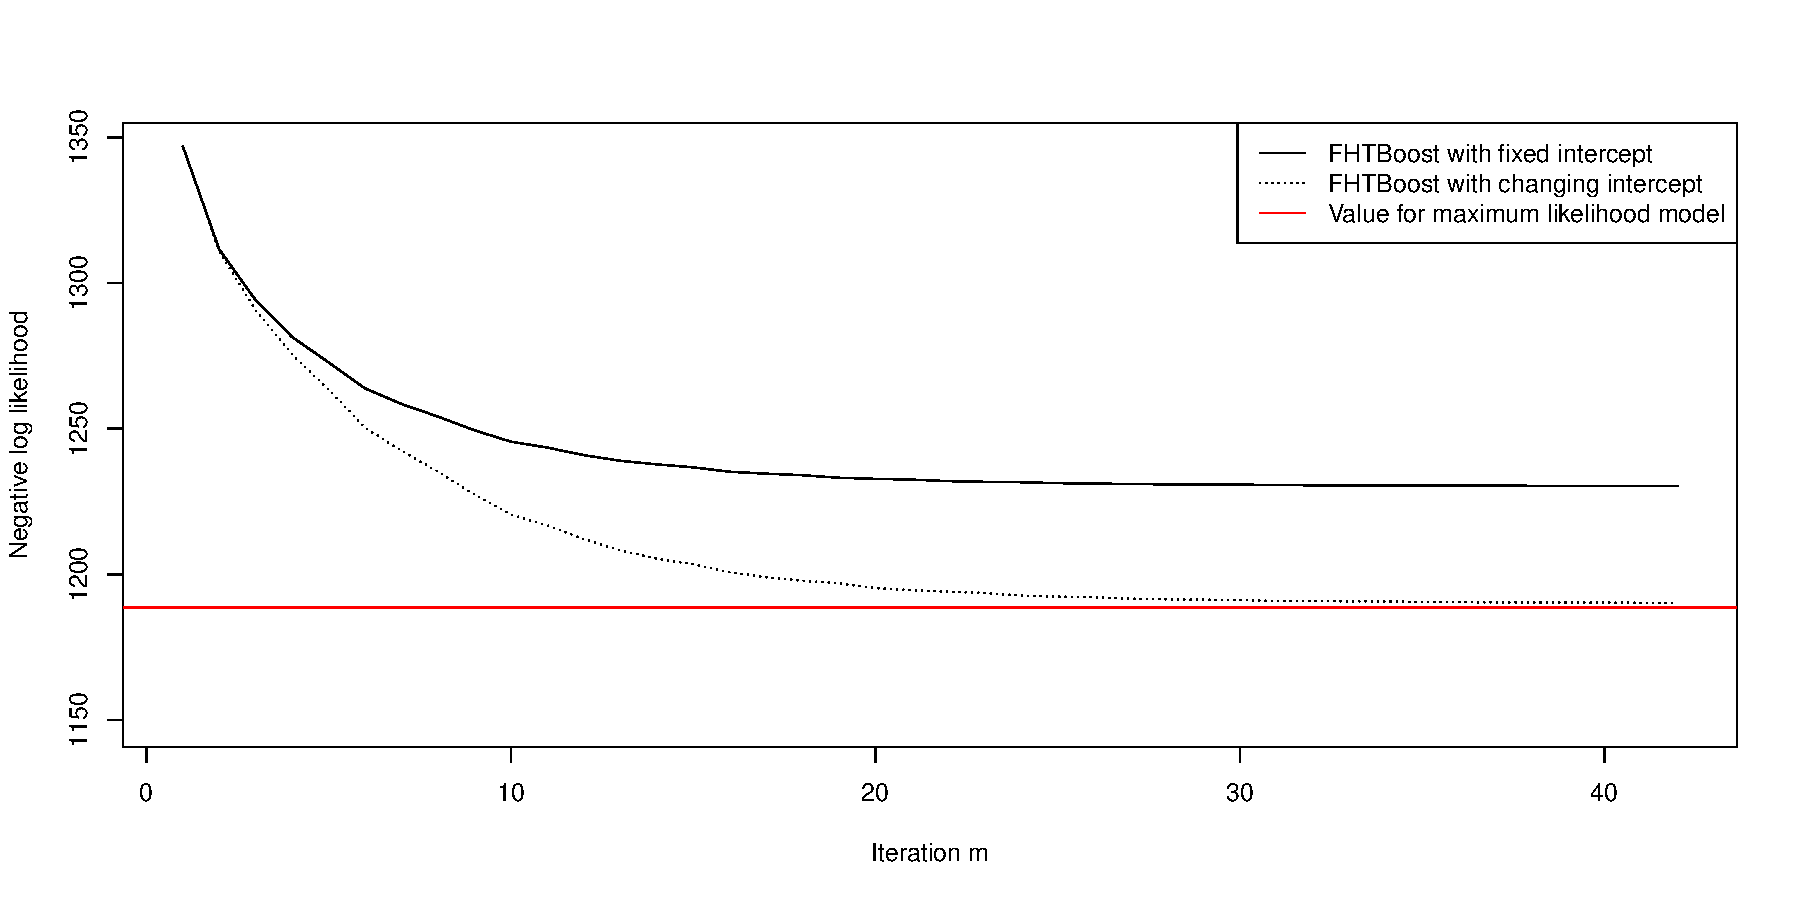
\includegraphics[scale=0.4]{figures/small_example.pdf}
\end{figure}
Figure \ref{fig:boosting-ML} shows a plot of the negative log likelihood of the data (in-sample loss) as a function of the iteration number $m$.
The solid black line shows negative log-likelihood for FHTBoost with a fixed intercept, i.e., the algorithm in the previous subsection.
With a fixed intercept, we only estimate the intercepts $\hat{\beta}_{0},\,\hat{\gamma}_{0}$ before we begin iterating, and so these intercepts are not changed in any of the boosting iterations.
The red line shows the negative of the maximum likelihood, obtained through numerical maximization of the joint maximum likelihood.
We can see in the figure \ref{fig:boosting-ML} that it quite clearly does not reach the maximum likelihood value, which is the solid red horizontal line.
The maximum likelihood intercepts are $\hat{\beta}^{\text{ML}}_{1,0}=1.98$ and $\hat{\beta}^{\text{ML}}_{2,0}=-1.02$, while running the boosting algorithm for $\mstop=42$ iterations produces estimates of the intercepts as $\hat{\beta}^{[\mstop]}_{0}=1.68$ and $\hat{\gamma}^{[\mstop]}_{0}=-0.71$, respectively.

We therefore see that to achieve the maximum likelihood, we have to modify the algorithm to incorporate updates in the intercepts while boosting.
To change the intercept in each boosting iteration, we can perform a new numerical maximization after each boosting step.
This means to perform the same kind of numerical maximization as is done initially, at the beginning of each iteration, using now the estimated additive predictors as offsets.
We denote the initially estimated intercept $\hat{\beta}_{1,0}$ as $\hat{\beta}_{1,0}^{[0]}$.
The intercepts in the additive predictors now become sums of boosted intercepts,
\begin{equation}
    \hat{\beta}_{0}=\hat{\beta}_{0}^{[0]}+\sum_{m=1}^{\mstop}\hat{\beta}_{0}^{[m]},
\end{equation}
and
\begin{equation}
    \hat{\gamma}_{0}=\hat{\gamma}_{0}^{[0]}+\sum_{m=1}^{\mstop}\hat{\gamma}_{0}^{[m]}.
\end{equation}
Here each $\hat{\beta}_{0}^{[m]}$ and $\hat{\gamma}_{0}^{[m]}$ are calculated in the intercept estimated in step $m$ of the boosting algorithm.

When introducing \textit{changing} intercepts, the algorithm was successful in recovering the maximum likelihood value and parameters.
See table \ref{table:ML} for the estimated parameter values, and graphically, in figure \ref{fig:boosting-ML}, where the convergence is plotted as a function of the number of boosting iterations.
\begin{table}\caption{Parameter values of a model which reaches ML}\label{table:ML}
\centering
\begin{tabular}{lcccccc}
\toprule
    & $\beta_{0}$ & $\beta_{1}$ & $\beta_{2}$ & $\gamma_{0}$ & $\gamma_{1}$ & $\gamma_{2}$ \\
\hline
Maximum likelihood estimate     &    1.98 &    0.10 &    0.21 &    -1.03 &    -0.09 &     0.12 \\
FHTBoost with fixed intercept                 &    1.68 &    0.10 &    0.18 &    -0.72 &    -0.06 &     0.09 \\
FHTBoost with changing intercept              &    1.97 &    0.10 &    0.18 &    -1.02 &    -0.09 &     0.12 \\
\bottomrule
\end{tabular}
\end{table}

In mboost, they seem to change the offset while boosting.
This must surely be a problem others have encountered while deriving boosting algorithms.

%The resulting survival times have the Kaplan-Meier plot shown in Figure \ref{fig:small-example-kaplan-meier}.
%\begin{figure}
%\caption{Kaplan-Meier plot of generated survival data from subsection \ref{subsec:algo-example}.}
%\label{fig:small-example-kaplan-meier}
%\centering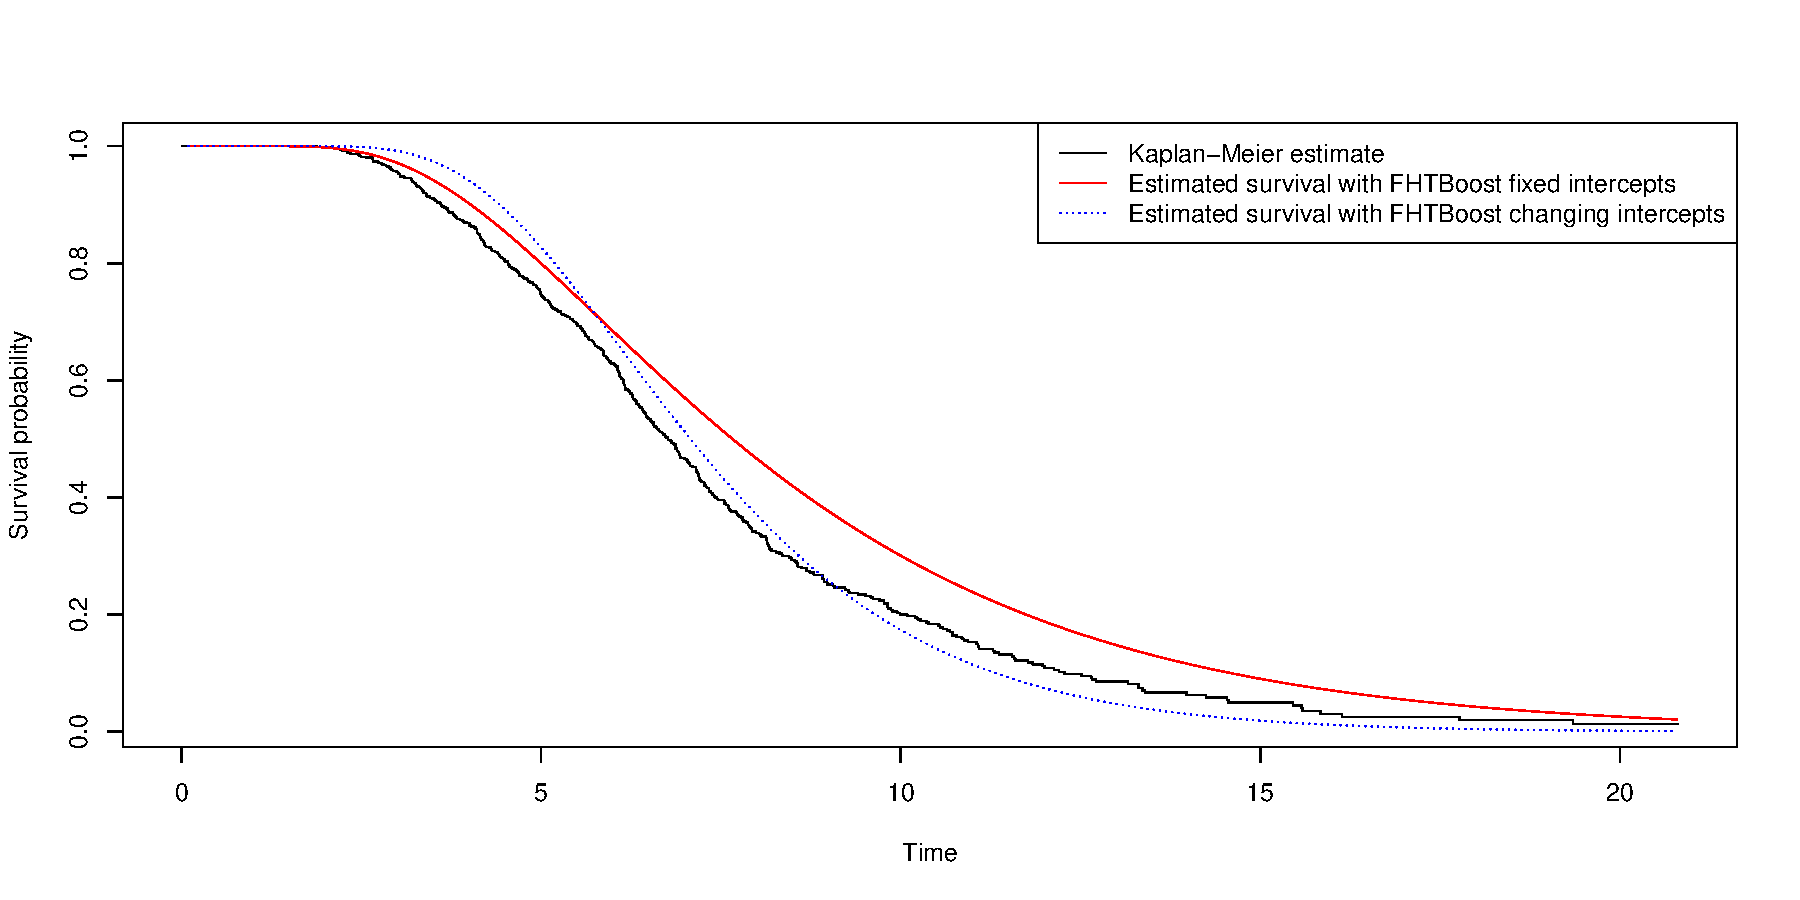
\includegraphics[scale=0.4]{figures/kaplan_meier_small.pdf}
%\end{figure}

\section{FHTBoost algorithm with changing intercept}\label{subsec:FHT-intercept}
%\begin{algorithm}
We modify algorithm \ref{algo:fhtboost}, where step \ref{algostep:FHT-end} is replaced by this step, where we incorporate changing intercepts for the additive predictors in each boosting iteration.
\label{algo:fhtboost-with-intercept}
\begin{enumerate}
    \setcounter{enumi}{12}
    \item
        Find which parameter should be included in the model,
        \begin{equation*}
            k^{[m]}=\argmin_{k\in\{1,2\}}\Delta\rho_k.
        \end{equation*}
        Include this component in the final model, by updating its additive predictor,
        \begin{equation*}
            \hat{\eta}^{[m]}_{k^{[m]}}=\hat{\eta}^{[m-1]}_{k^{[m]}}+\nu\cdot\hat{h}^{[m]}_{k^{[m]},\,j^{[m]}}(x),
        \end{equation*}
        while for the other component $k\neq k^{[m]}$, set the additive predictor for this iteration to be the same as previous iteration
        \begin{equation*}
            \hat{\eta}^{[m]}_{k}=\hat{\eta}^{[m-1]}_{k}.
        \end{equation*}
        Find the best numerical constant to add to the intercept of the selected additive learner,
        \begin{equation}
            c=\argmin_c \err\left(\hat{\boldeta}^{[m]}+c\right)
        \end{equation}
        Add this $c$ to the selected parameter
        \begin{equation}
            \hat{\beta}_{k^{[m]},0}\gets\hat{\beta}_{k^{[m]},0}+c.
        \end{equation}
\end{enumerate}
%\end{algorithm}

\section{Conclusion thoughts choices}
\todo[inline]{Write a conclusion from the example: The algorithm with updating intercept seems better, as it should not be shrunk towards 0 \citep{ESL}.}

    \chapter{Evaluation measures}

\section{Difference in deviance}
Difference in deviance is a measurement for comparing models of the same type, e.g., between different parameter vectors of an FHT model.
The objective of the measurement is to assess how much the model improves when adding covariates.
We estimate the parameters of the FHT model on the training set.
When doing so, we first find the intercepts of the covariate vectors, $\beta_0$ and $\gamma_0$, respectively,
and the initial covariate vectors, i.e., the covariate vectors before starting boosting, are
\begin{equation*}
    \hat{\bbeta}^{[0]}_{\text{train}}=(\beta_0^{[0]},0,0,\ldots,0)
\end{equation*}
and
\begin{equation*}
    \hat{\bgamma}^{[0]}_{\text{train}}=(\gamma_0^{[0]},0,0,\ldots,0)
\end{equation*}
We denote the concatened vector of these as
\begin{equation*}
    \hat{\btheta}^{[0]}_{\text{train}}=\left(\bbeta^{[0]},\bgamma^{[0]}\right).
\end{equation*}
We call this the \textit{null model}, because it incorporates no covariate information, and will therefore predict and perform the same for every individual.
Similarly, the fully estimated covariate vectors, boosted with $\mstop$ steps, on the training set, are
\begin{equation*}
    \hat{\bbeta}^{[\mstop]}_{\text{train}}=(\beta_0^{[\mstop]},\beta_1^{[\mstop]},\beta_2^{[\mstop]},\ldots,\beta_p^{[\mstop]})
\end{equation*}
and
\begin{equation*}
    \hat{\bgamma}^{[\mstop]}_{\text{train}}=(\gamma_0^{[\mstop]},\gamma_1^{[\mstop]},\gamma_2^{[\mstop]},\ldots,\gamma_d^{[\mstop]}).
\end{equation*}
Again let their concatenation be denoted as
\begin{equation*}
    \hat{\btheta}^{[\mstop]}_{\text{train}}=\left(\hat{\bbeta}^{[\mstop]}_{\text{train}},\hat{\bgamma}^{[\mstop]}_{\text{train}}\right).
\end{equation*}
We call this the model.
The deviance of a model $\btheta$ is
\begin{equation}
    \text{dev}(\btheta)=2l(\btheta),
\end{equation}
where $l(\btheta)$ is the log-likelihood value attained by an estimated covariate vector $\btheta$.
Deviance is used a lot in the generalized linear models (GLM) framework, where there exist a lot of results.
The difference of deviance between two models $\btheta_1$ and $\btheta_2$ is
\begin{equation}
    d=\text{dev}(\btheta_1)-\text{dev}(\btheta_2)=2l(\btheta_1)-2l(\btheta_2)=2\left(l(\btheta_1)-l(\btheta_2)\right).
\end{equation}
In our case, the likelihood of the null model on the test set is
\begin{equation}
    l^{\text{test}}\left(\hat{\btheta}^{[0]}_{\text{train}}\right).
\end{equation}
The notation here is a bit overloaded to make it explicitly clear that the covariate vector is estimated based on the \textit{training} set, and that the log-likelihood value is calculated on the \textit{test} set.
We wish to measure how much better $\hat{\btheta}_{\text{train}}^{[\mstop]}$ explains the variation in the test set than $\hat{\btheta}_{\text{train}}^{[0]}$ does.
Further, the trained model, with covariates, is a model $\hat{\btheta}^{[\mstop]}_{\text{train}}$, i.e., a model boosted with $\mstop$ steps.
The estimated model which incorporates covariates has a likelihood of
\begin{equation}
    l^{\text{test}}\left(\hat{\btheta}^{[\mstop]}_{\text{train}}\right).
\end{equation}
It is conventional to put the least complex model first, and the more complex model last.
Since a more complex model should achieve a better, and thus higher, log-likelihood, the difference of deviance should be negative. 
Hence the difference in deviance between a fitted model and the null model containing no covariates is
\begin{equation*}
    d=2\left(l^{\text{test}}\left(\hat{\btheta}^{[0]}_{\text{train}}\right)-l^{\text{test}}\left(\hat{\btheta}^{[\mstop]}_{\text{train}}\right)\right).
\end{equation*}
The performance of a model is good when $d$ is small, meaning ``very negative.''
In some of the results in this section, we end up with a \textit{positive} difference of deviance.
This means that the null model achieved a higher log-likelihood value than the fully estimated model.
This is the typical effect of overfitting, where the model follows too much random variability in the training set, and performs badly on the test set.


\section{Variable selection}
As shown in section \ref{sec:variable-selection}, a component-wise gradient boosting algorithm, such as FHTBoost,
performs data-driven variable selection.

We denote a variable selected by the algorithm as ``positive,'' or $P$ for short, and a variable that is not selected as ``negative,'' or $N$ for short.
Since we know which variables actually affect the response, we know how many of the variables selected are selected correctly, in the sense
that they are selected and they have an effect. We call these ``true positives,'' or $TP$ for short.
Similarly, we know which variables do not affect the response, and so we can calculate the number of non-informative variables
which were not selected, i.e., true negative, or $TN$ for short.
Furthermore, we say that variables which have been selected but which do not actually have an effect, are false positives, $FP$.
Similarly, false negatives, $FN$, are variables which do actually have an effect, but which were not selected in the boosting model.
Here follows the definition of three metrics that we use to determine how well the model performs variable selection.

\textbf{Sensitivity} measures the proportion of the selected variables which are informative.
Ideally, this is 1.
\begin{equation}\label{eq:sensitivity}
    \text{Sensitivity}=\frac{TP}{P}
\end{equation}

\textbf{Specificity} measures the proportion of variables \textit{not} selected which were not informative.
Ideally, this is 1.
\begin{equation}\label{eq:specificity}
    \text{Specificity}=\frac{TN}{N}
\end{equation}

\textbf{False discovery rate} measures the proportion of selected variables which are in truth not informative.
Ideally, this is 0.
\begin{equation}\label{eq:accuracy}
    \text{FDR}=\frac{FP}{FP+TP}
\end{equation}

\section{Brier score}
The Brier score \citep{brier1950} was first introduced as a way to measure the accuracy of weather forecasts, and then translated into survival analysis \citep{graf}.
Let us first consider, for ease of presentation, the case with no censoring.
We have $N_{\text{test}}$ individuals in a test set.
We denote their observed survival times by $t_i$, and their covariate vector as $\x_i$, as usual, with $i=1,\ldots,N_{\text{test}}$. The Brier score aims at evaluating how well the estimated patient specific survival probability $\hat{\pi}(t^*|\x)$, obtained from a prediction model, is able to predict the event status $I(t>t^*)$ of an individual at a given time $t^*$.
The error made in predicting the event status $I(t>t^*)$ for a patient in the test set can be given as
\begin{align*}
BS(t^*)&=\frac{1}{N_{\text{test}}}\sum_{i=1}^{N_{\text{test}}}\left(I(t_i>t^*)-\hat{\pi}(t^*|\x_i)\right)^2 \\
    &=\frac{1}{N_{\text{test}}}\sum_{i=1}^{N_{\text{test}}}\left[\hat{\pi}(t^*|\x_i)^2I(t_i\leq t^*)+(1-\hat{\pi}(t^*|\x_i))(I(t_i>t^*)\right].
\end{align*}
In the first formulation, the Brier score looks like a version of an RSS measure, where one sums the squared error between the observed event and the estimated probability.
In the case of censored data, the above is not enough.

The Brier score was adapted to handle censored survival times by \citet{graf}, assuming independent censoring.
They showed that the loss of information due to censoring can be accounted for by using an inverse probability of censoring weighting \citep{bovelstadborgan}.
This version of the Brier score for censored data is defined as
\begin{equation*}
    BS^c(t^*)=\frac{1}{N}\sum_{i=1}^N\left[\frac{\hat{\pi}(t^*|\x_i)^2I(t_i\leq t^*,\delta_i=1)}{\hat{G}(t_i)}+\frac{(1-\hat{\pi}(t^*|\x_i))(I(t_i>t^*)}{\hat{G}(t^*)}\right].
\end{equation*}
Here $\hat{G}$ is the Kaplan-Meier estimate of the censoring distribution, defined as
\begin{equation*}
    \hat{G}(t)=\prod_{i\in \overline{R}(t)}\left(1-\frac{1-\delta_i}{\sum_{i=1}^NY_i(t)}\right),
\end{equation*}
where $Y_i(t)$ is an indicator of whether individual $i$ is at risk at time $t$, and where $\overline{R}(t)$ is the set of individuals \textit{not} at risk at time $t$, i.e.,
\begin{equation*}
    \overline{R}(t)=\{i\colon t_i<t,i=1,2,\ldots,N\}.
\end{equation*}

\subsection{$R^2$ measure based on Brier score}
The Brier score may also be used to define an $R^2$ measure, where one can benchmark the performance of a fitted model to a so-called null model, i.e., one where each regression coefficient is set to zero. A measure of explained variation can be found by calculating the gain in accuracy when adding covariates. Thus we define the Brier $R^2$ measure as
\begin{equation*}
    R^2_{\text{Brier}}(t^*)=1-\frac{BS^c(t^*)}{BS^c_0(t^*)},
\end{equation*}
where $BS^c_0(t^*)$ is the Brier score for the null model.
One advantage with $R^2_{\text{Brier}}$ is that it adjusts for variation due to the specific data under study, which the Brier score itself does not \citep{bovelstadborgan}.
Note, though, that this $R^2$ measure is model specific, since it is based on a comparison between two models of the same kind.
It should therefore be used to assess how well a specific model, such as FHTBoost, improves with covariates.
However, to compare the predictive power of different models, such as FHTBoost and CoxBoost, one should use the ``raw'' Brier score $BS^c(\cdot)$.

\subsection{Integrated Brier score}
\todo[inline]{Explain!!}
\begin{align*}
    \text{IBS}(t_{\text{start}}, t_{\text{end}})&=\int_{t_{\text{start}}}^{t_{\text{end}}}BS^c(t)\d t \\
    &\approx\sum_{i}BS^c(t_i)\cdot(t_{i+1}-t_{i}).
\end{align*}


    \chapter{Simulation study}
After developing FHTBoost (see chapter \ref{ch:FHTboost}), we wish to verify that it works, i.e. that it has predictive power and selects correct variables.
Not only that, but we wish to see which of the two versions of the algorithm works best, namely the fixed intercept version and the version with an iteratively changing intercept.

One way to verify that a statistical estimation method works, is to test it on simulated data.
Simulation studies are used for many different purposes, but a particularly common purpose is to simulate survival data from the ``true model'' (in this case, our first-hitting-time model), for which we know the true values of the parameters.
We can then use our developed method to estimate these parameters, and see how well it recovers the true parameters in the final model, and how well the model fits the simulated data.
The model should fit the simulated data well, because the data generating mechanism \textit{is} the model.
In this chapter, we simulate data, use FHTBoost to estimate models, and assess the performance of these models.
The boosting algorithm has two main purposes:
Selection of variables, and minimizing test error.
To assess the test/generalization error, we calculate the difference of deviance on the test set.
To assess variable selection, we look at some well known metrics.

\section{Simulation design}
In this chapter we describe two scenarios, a highly correlated scenario and an uncorrelated scenario. 
The purpose of each scenario is to first generate survival data from an FHT mechanism, based on known true parameters, then use FHTBoost to estimate the parameters of the model, and then finally to assess the model's performance on this data.
In both scenarios, we generate a high-dimensional covariate matrix $\X$ consisting of covariate vectors
\begin{equation}
    \x_1,\x_2,\ldots,\x_{p_1},
\end{equation}
which is supposed to mimic gene expression data.
We also have a low-dimensional covariate matrix $\Z$, which similarly consist of covariate vectors
\begin{equation}
    \z_1,\z_2,\ldots,\z_{p_2},
\end{equation}
and which is supposed to mimic clinical measurements.
The motivation for this dichotomy is discussed in subsection \ref{subsec:FHT-combine}.
We link each covariate to a parameter in a parameter vector.
We let $\X$ correspond to $\bbeta$, and $\Z$ correspond to $\bgamma$.
This allows us to test the variable selection performance of FHTBoost.
In each parameter vector, we set only a small number of parameters to a non-zero value, and we set all the rest to zero.
Thus only a very small number of covariates will have an effect.
Given these parameter vectors and covariate matrices, we calculate a specific $y_{0,i}$ and a specific $\mu_i$ for each individual $i$, where $i=1,2,\ldots,N$, and where $N$ is the size of the data set.
From the FHT perspective, discussed previously in section \ref{fht-idea} and onward, these are parameters representing the health process of each individual.
To reiterate, an individual $i$ has a stochastic health process, specifically a Wiener process with an initial level $y_{0,i}$ and a drift $\mu_i$.
When the health process hits 0, it causes the event for the individual.
Since the FHT of a Wiener with health level $y_{0,i}$ and drift $\mu$ is $\IG(y_{0,i},\mu_i)$, then also the individual's lifetime follows this distribution $\IG(y_{0,i},\mu_i)$.
This relationship allows us to easily draw a lifetime for each individual from its respective inverse Gaussian distribution.

It is important to evaluate an estimated model's performance on a separate and unseen test set.
Each training set will be generated by drawing $N=500$ individuals as described above, with a specific seed.
Since we are simulating, it is simple to generate a test set by drawing from a unique seed.
We are therefore also able to decide the size of the test set.
We set $N_{\text{test}}=1000$ observations.

We generate $B\approx500$ data sets by drawing survival data according to algorithm \ref{algo:FHT-sim}.
In each data set there are $N=500$ observations. 
We treat each data set as a separate training data set.
To estimate a model based on a training set, we first perform repeated 5-fold cross validation procedure (see subsection \ref{subsec:K-fold}), with 5 repeats.
As shown in subsection \ref{subsec:iterations}, this provides a reasonably variance reduced estimate of $\mstop$ (near the ``true'' $\mstop$).
We then estimate a model based on the entire training set, by running FHTBoost with $\mstop$ number of iterations.

To simulate the covariate matrices $X$ and $Z$ we will use Algorithm \ref{algo:clinical-sim}, which is a method for simulating clinical and gene data together.
We specify the different correlations for the covariate matrices.
We specify the true parameter vectors, $\bbeta$ and $\bgamma$.
For each scenario, we create $B$ data sets.
For each of these, we estimate FHT parameters using FHTBoost.

For each data set $D_b$, we first draw data (with a specific seed to ensure reproducibility).
We do this by drawing covariate matrices $\X$, $\Z$ from Algorithm \ref{algo:clinical-sim}.
Then we combine these with the true covariate matrices to get vectors $\y_0$ and $\mathbf{\mu}$ of initial value of the health process, and drift, respectively.
Then we draw from the Inverse Gaussian distribution according to Algorithm \ref{algo:FHT-sim}, obtaining $N$ right-censored lifetimes, i.e., $N$ tuples $(t_i,d_i)_{i=1,\ldots,N}$.
With these tuples, then, we can do a run with the FHT boosting algorithm. We first use repeated K-fold cross-validation to find the optimal number of boosting steps, $m_{\text{stop}}$.
Then we estimate the model on the whole of this training set.
Then we validate this model on a test set of size $N_{\text{test}}$.
The data here are drawn in the exact same manner as the training data, again with a specific seed for reproducibility.
We first discuss the algorithms we use to generate FHT survival data.

\section{Simulation of survival data from an IG FHT distribution}\label{sec:simulate-IG-data}
We wish to simulate survival times $(\ti)_{i=1}^N$ with censoring.
We first draw $N$ uncensored survival times $\{\tilde{t}_i\}_{i=1}^N$ from a survival time distribution $f(\cdot)$.
If this distribution has a closed form probability distribution function, we can draw from it directly, and this is the case for us.
To implement censoring of the data, we draw censoring times $w_i\sim f(\cdot),i=1,\ldots,N$ from some other lifetime distribution where the parameters do \textit{not} depend on covariates.
Thus the observed survival times are
\begin{equation}
    t_i=\min(\tilde{t}_i,w_i),
\end{equation}
as we have seen before.
The corresponding censoring indicator, $d_i$, is then set equal to 1 if the actual survival time was observed, i.e., if $\ti<w_i$.
We end up with a data set
\begin{equation}
    D=(\x_i,\,\z_i,\,t_i,\,d_i)_{i=1}^N.
\end{equation}
Note that this prcedure simulates censored time under independent censoring, since indeed the censoring times are independent of the survival times.
See \ref{algo:FHT-sim} for a schematic overview of the algorithm.

\begin{algorithm}
\caption{Generating survival data from Inverse Gaussian FHT distribution}
\label{algo:FHT-sim}
\begin{enumerate}
    \item Obtain the design matrices $\X$, $\Z$ and the true parameter vectors $\bbeta$ and $\bgamma$.
    \item\label{algo:FHT-sim-step-cens} Specify a censoring time distribution.
    \item Calculate the distribution parameters $y_0$ and $\mu$ using the link functions,
        \begin{align*}
            y_0&=\exp(\bbeta^T\X)=\exp\left(\beta_0+\sum_{j=1}^p\beta_jx_j\right), \\
            \mu&=\bgamma^T\Z=\gamma_0+\sum_{j=1}^d\gamma_jz_j.
        \end{align*}
    \item Draw $N$ uncensored survival times $(\tilde{t}_i)_{i=1}^N$ from $\IG(\boldsymbol{\mu},\boldsymbol{y}_0)$, where
        \begin{equation*}
            \tilde{t}_i\sim\IG(\mu_i,\y_{0,i}).
        \end{equation*}
    \item Draw $N$ censoring times $(w_i)_{i=1}^N$ from the censoring time distribution specified in step \ref{algo:FHT-sim-step-cens}.
    \item Right censor the survival times by choosing
            \begin{equation*}
                t_i=\min(\tilde{t}_i,w_i).
            \end{equation*}
          The censoring indicator on whether observation $i$ was observed or not is then
          \begin{equation*}
            d_i=I(t_i=\tilde{t}_i).
          \end{equation*}
    \item The simulated data set is $D=(t_i,\,d_i)_{i=1}^N$.
\end{enumerate}
\end{algorithm}

\section{Generating correlated clinical and gene expression data}
To create a realistic scenario where we have data looking like gene expression data and clinical data, we need to define a proper correlation structure.
We can draw covariate matrices from a normal distribution with a suitable covariance matrix.

We consider a scenario where we have a covariate matrix $X$ consisting of $p$ gene expressions, and a covariate matrix $Z$ consisting of $d$ clinical measurements.
We can imagine that some of the genes in $X$ are highly correlated.
One way to imagine this is to imagine that we have blocks of genes,
where inside one block, the genes are highly correlated, whereas genes in one block are not correlated to other genes.
In addition, one block of genes might affect a block of clinical variables as well.

We specify a number of blocks $B$. A given block $b,b=1,2,\ldots,B$, contains a certain number of genes, $G_b$, which are correlated to each other.
It also contains a certain number of clinical measurements, $C_b$. These measurements are correlated to each other, and to the genes in the block.

After setting up the block structure, we 
\todo[inline]{Finish this}

There are three types of correlations.
1. Within each block of genes. Defaults to 0 for genes not belonging to any block.
2. Between clinical predictors in each pathway
3. Between the clinical and molecular predictors in each pathway

Algorithm \ref{algo:clinical-sim} contains a schematic overview.

\begin{algorithm}
\caption{Generating correlated clinical and gene expression data}
\label{algo:clinical-sim}
\begin{enumerate}
    \item Lorem ipsum.
\end{enumerate}
\end{algorithm}

\section{Scenarios}
\subsection{Scenario 1: Uncorrelated case}
We generate a data set of size $N_{\text{scenario}}=500$, and parameter vectors of size $10000$ and $15$, respectively.
We let $\bbeta$ be a large vector of size $p=10001$, and $\bgamma$ be a small vector of size $d=16$.
We first discuss the size of the parameter effects.
The parameter vector $\bbeta$ is linked to the initial level $y_0$ by an exponential link function.
Consequently, each parameter effect is \textit{multiplicative} instead of additive.
A large gene expression value can therefore potentially cause a large change in $y_0$.
Since there are 35 elements of $\bbeta$ which are informative, there is a reasonable chance of such extreme values occurring in $y_0$.
Because of this, we had trouble setting up simulations in which there was much signal from the underlying parameter vector.
Therefore we choose 0.1 for the informative parameter effects $\beta_j,j=1,2,\ldots,35$.
The parameter sizes on the drift might also appear rather small, at 0.1, but this effect is linear with time.
By having a relatively low effect per time unit, we ensure that the lifetimes are not too short.
These two considerations in mind made us achieve a decent simulation setup.
Specifically, we set the intercept term in $\bbeta$ to be 2.0, and the following $p_1=35$ elements to be 0.1.
We set all other elements to 0.
For $\bgamma$, we set the intercept term to be -1.
In similar fashion as in $\bbeta$, we let the first 5 elements in $\bgamma$ have a non-zero value of -0.1, while we set the remaining 10 elements to 0.
Hence, the true parameter vectors are
\begin{align*}
    \bbeta=\left(2.0, \underbrace{0.1, 0.1, \ldots, 0.1}_{\text{length 35}}, \overbrace{0, 0, \ldots, 0}^{\text{length 9965}}\right) \\
    \bgamma=\left(-1.0, \underbrace{0.1, 0.1, \ldots, 0.1}_{\text{length 5}}, \overbrace{0, 0, \ldots, 0}^{\text{length 10}}\right)
\end{align*}
We draw $X$ and $Z$ from Algorithm \ref{algo:clinical-sim} for drawing clinical and gene data, with $B=0$ blocks.
We specify that all correlations are 0, meaning no covariate correlates with any other.
We generate $B=500$ data sets from this algorithm, where we set the seed at the beginning of each simulation.
Having now a data set $D_b$, we run cross validation on this data set to find the optimal iteration number $m_{\text{stop}}$.
We then run a boosting algorithm with $m_{\text{stop}}$ steps on the training set, to estimate parameters.
We will discuss the results in the next section, but we first describe the other scenario.

\subsection{Scenario 2: Correlated}
Consider now a scenario where we wish to have high correlation.
We have blocks of genes which are correlated, meaning the genes comprising one are correlated.
Furthermore, we let the genes in a block of genes be correlated with a (smaller) block of clinical measurements.
Finally, the clinical measurements are correlated.
All these correlations are set to 0.7.
The main purpose of the algorithm is to specify the covariance matrix before drawing the data.

There are three types of correlations.
1. Within each block of genes. Defaults to 0 for genes not belonging to any block.
2. Between clinical predictors in each pathway
3. Between the clinical and molecular predictors in each pathway

\section{Results}
After having estimated an FHT model on the training set, we assess the performance of the model on the test set.
We calculate the difference of deviance.
To assess the variable selection of the model, we calculate metrics for the variables selected based on the training set.
We count $TP$, the number of informative covariates which were selected in the estimated boosting model, and $TN$, the number of non-informative covariates which were selected in the model.
Based on these numbers, we calculate the metrics discussed in Section \ref{sec:variable-selection}, namely Sensitivity, Specificity and False Discovery Rate.
Let us now consider the results of each scenario.

\subsection{Uncorrelated case}
\subsubsection{Test set performance/model fit}
The most evident result is that, in contrast to our expectation, the fixed intercept version of FHTBoost seems to perform on average better than that with updating intercept (see Table \ref{table:uncorrelated-deviance}).
The mean difference of deviance on the updating intercept version is -92.0, while it is -130.1 on the fixed intercept version.
Despite the large variability (see min, max and standard deviation in Table \ref{table:uncorrelated-deviance}) in the distributions of the difference of deviance results, the difference between the fixed intercept and the changing intercept are noticeable.
This is perhaps most apparent in Figure \ref{fig:simulation-uncorrelated-deviances-boxplot}.
In addition, the fixed intercept version always performs better than the null model, while there are a few cases in which the updating intercept version does not (Table \ref{table:uncorrelated-deviance}, row "min", and Figure \ref{fig:simulation-uncorrelated-deviances-boxplot}).
In other words, all models estimated using the fixed intercept version performed better than their null models, whereas this is not the case for the version with a changing intercept.
This can be a consequence of overfitting.
Moving the intercept allows the model to fit the training data too well.
We now consider the variable selection metrics.

\begin{table}
\caption{Difference of deviance results for FHTBoost, uncorrelated case}
\label{table:uncorrelated-deviance}
\centering
\begin{tabular}{l|rr}
\toprule
& Updating & Fixed \\
\hline
Mean               &  -92.0  & -130.1  \\
Standard deviation &   41.8  &   40.7  \\
Minimum            & -233.6  & -255.2  \\
Maximum            &    7.2  &   -5.7  \\
\bottomrule
\end{tabular}
\end{table}

\begin{figure}
\caption{Boxplot for difference in deviance for the two intercept variants, non-correlated scenario}
\label{fig:simulation-uncorrelated-deviances-boxplot}
\centering
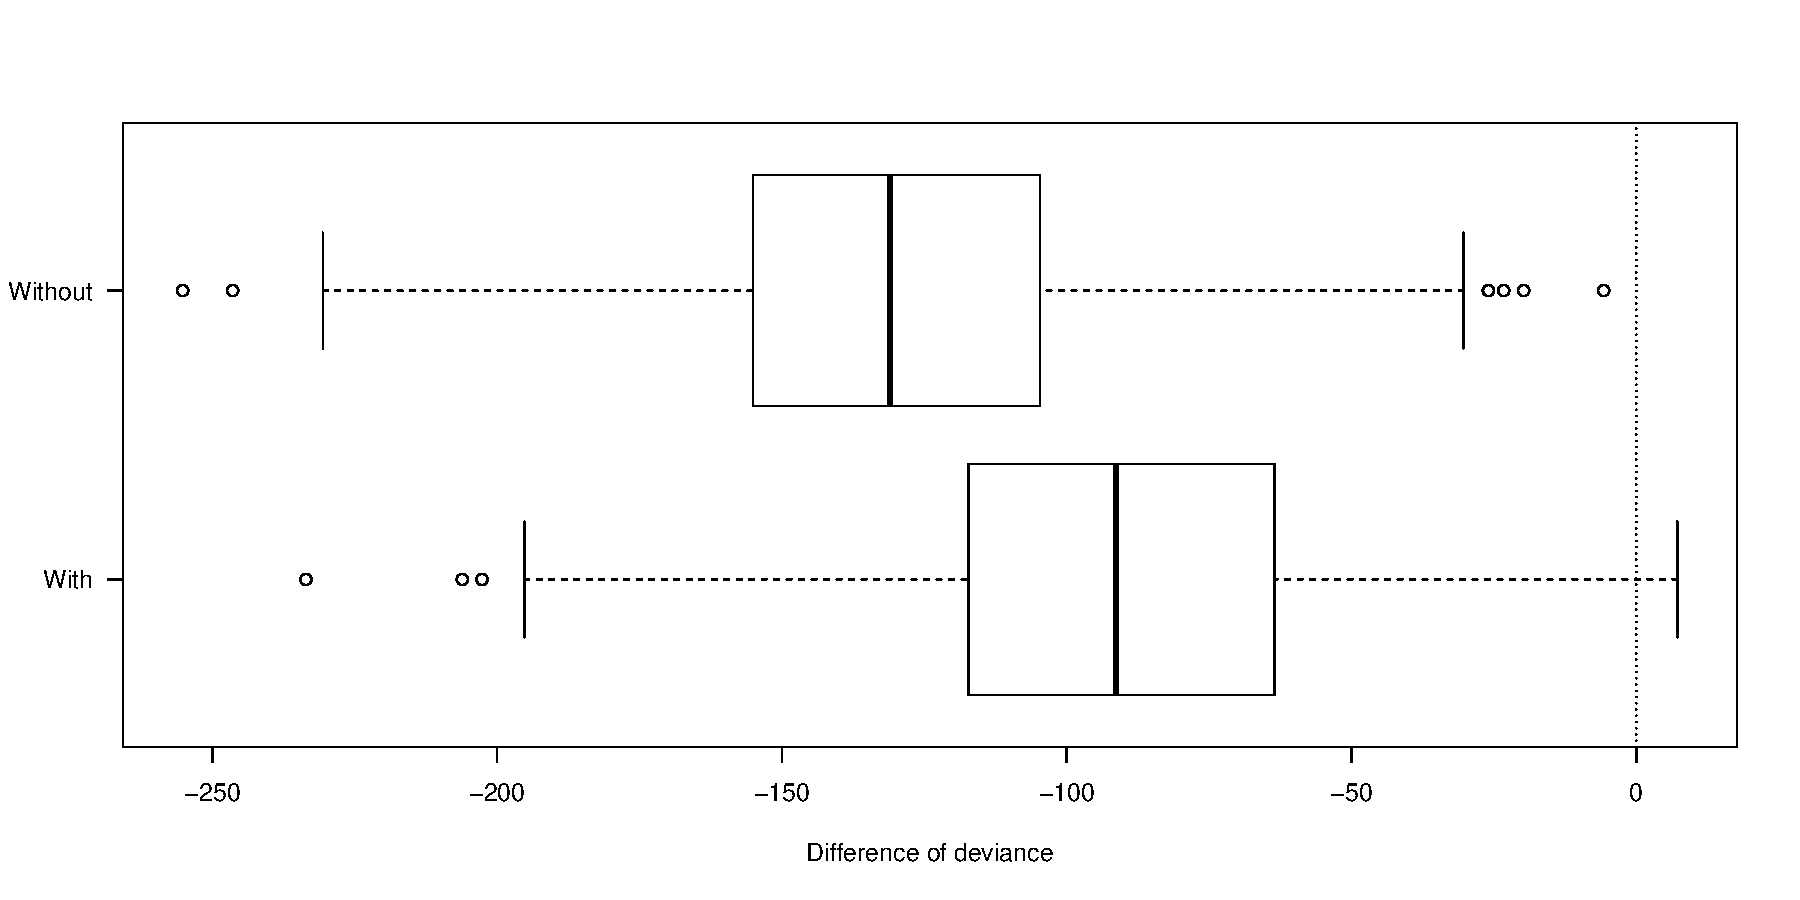
\includegraphics[scale=0.4]{deviances_simulation.pdf}
\end{figure}

\subsubsection{Variable selection}
Let us contrast the two versions of FHTBoost in terms of variable selection as well.
This scenario has 35 informative gene covariates and 5 informative clinical covariates.
Since the changing intercept version has a rather low number of iterations, with a mean of 15.8, it is usually impossible to get anywhere near perfect on these metrics, as at most one new parameter is selected in each iteration, and we have 40 informative covariates in total from the two vectors.
Since the covariate vector is estimated on the training data, a likely explanation is that the changing intercept captures more of the variation in the training data.
In doing so, there is less variation to be explained by the covariates, and hence the boosting algorithm will start to overfit more quickly.

Furthermore, we are considering the sensitivity and specificity on both covariate vectors at the same time.
Since we are only selecting a covariate for either $\bbeta$ or $\bgamma$, these scores will depend on each other.

\begin{table}
\caption{High dimensional (genomic) part: Performance of FHTBoost in terms of variable selection, uncorrelated case}
\label{table:uncorrelated-y0}
\centering
\begin{tabular}{l|cc|cc}
\toprule
& \multicolumn{2}{c}{Updating} & \multicolumn{2}{c}{Fixed} \\
& Mean & Standard error & Mean & Standard error \\
\hline
Sensitivity & 0.190 & (0.090) & 0.452 & (0.162) \\
Specificity & 1.000 & (0.000) & 0.997 & (0.002) \\
FDR         & 0.310 & (0.176) & 0.613 & (0.144) \\
\bottomrule
\end{tabular}
\end{table}

\begin{table}
\caption{Low dimensional (clinical) part: Performance of FHTBoost in terms of variable selection, uncorrelated case}
\label{table:uncorrelated-mu}
\centering
\begin{tabular}{l|cc|cc}
\toprule
& \multicolumn{2}{c}{Updating} & \multicolumn{2}{c}{Fixed} \\
& Mean & Standard error & Mean & Standard error \\
\hline
Sensitivity & 0.741 & (0.232) & 0.958 & (0.099) \\
Specificity & 0.943 & (0.110) & 0.638 & (0.291) \\
FDR         & 0.091 & (0.144) & 0.375 & (0.192) \\
\bottomrule
\end{tabular}
\end{table}

\begin{table}
\caption{Optimal iteration number $\mstop$ results for FHTBoost, uncorrelated case}
\label{table:uncorrelated-mstop}
\centering
\begin{tabular}{l|rr}
\toprule
& Updating & Fixed \\
\hline
Mean               &  15.8  &  63.8  \\
Standard deviation &   6.4  &  26.5  \\
Minimum            &     2  &     2  \\
Maximum            &    39  &   160  \\
\bottomrule
\end{tabular}
\end{table}

Consider first the result of the version in which the intercept is changed in each step.
Both covariate vectors have a very high specificity, which measures the amount of true negatives which are correctly classified as negatives, i.e., not selected.
The changing intercept version has a mean specificity of 1.00.
It also has a mean false discovery rate of 0.316.
Thus there is about a one in three chance that it selects a variable which is not actually informative.
The sensitivity, i.e., the ratio of correctly selected informative variables, has a mean of only 0.190.
This means that a large proportion of the informative covariates are not selected.
For $\bgamma$, which is related to the clinical covariates, a much higher specificity is attained, with a mean of 0.943.
Even though the parameter effects on the drift are rather small, the informative covariates are often correctly selected.
Furthermore, the false discovery rate here is very low, with a mean of 0.091.

Now consider the results of the fixed intercept version.
For the $\bbeta$ covariate vector, a higher proportion of informative covariates are selected, with a mean sensitivity of 0.452.
The mean specificity is 0.997.
Simultaneously, a larger mean false discovery rate of 0.613 is not good:
This means that more than half of all selected variables should be expected to be false positives.
At the same time, a very good sensitivity is achieved on the $\bgamma$ covariate vector, with a mean of 0.958, and a good specificity with a mean of 0.638.
The false discovery rate on $\bgamma$ is slightly above one in three, with a mean of 0.375.

\subsubsection{Summary}
\todo[inline]{Summarize}

\subsection{Correlated case}
We now consider the results for the correlated simulation study.

\subsubsection{Test set performance/model fit}
We observe that the mean deviance is very slightly better for the fixed intercept version, and with better extreme values, both minimum and maximum.
See Figure \ref{fig:simulation-correlated-deviances-boxplot} for a boxplot of these deviances.
However, it is very close, so it is difficult to say that there is any difference in the model fit for these two versions.

\begin{figure}
\caption{Boxplot for difference in deviance for the two intercept variants, correlated scenario}
\label{fig:simulation-correlated-deviances-boxplot}
\centering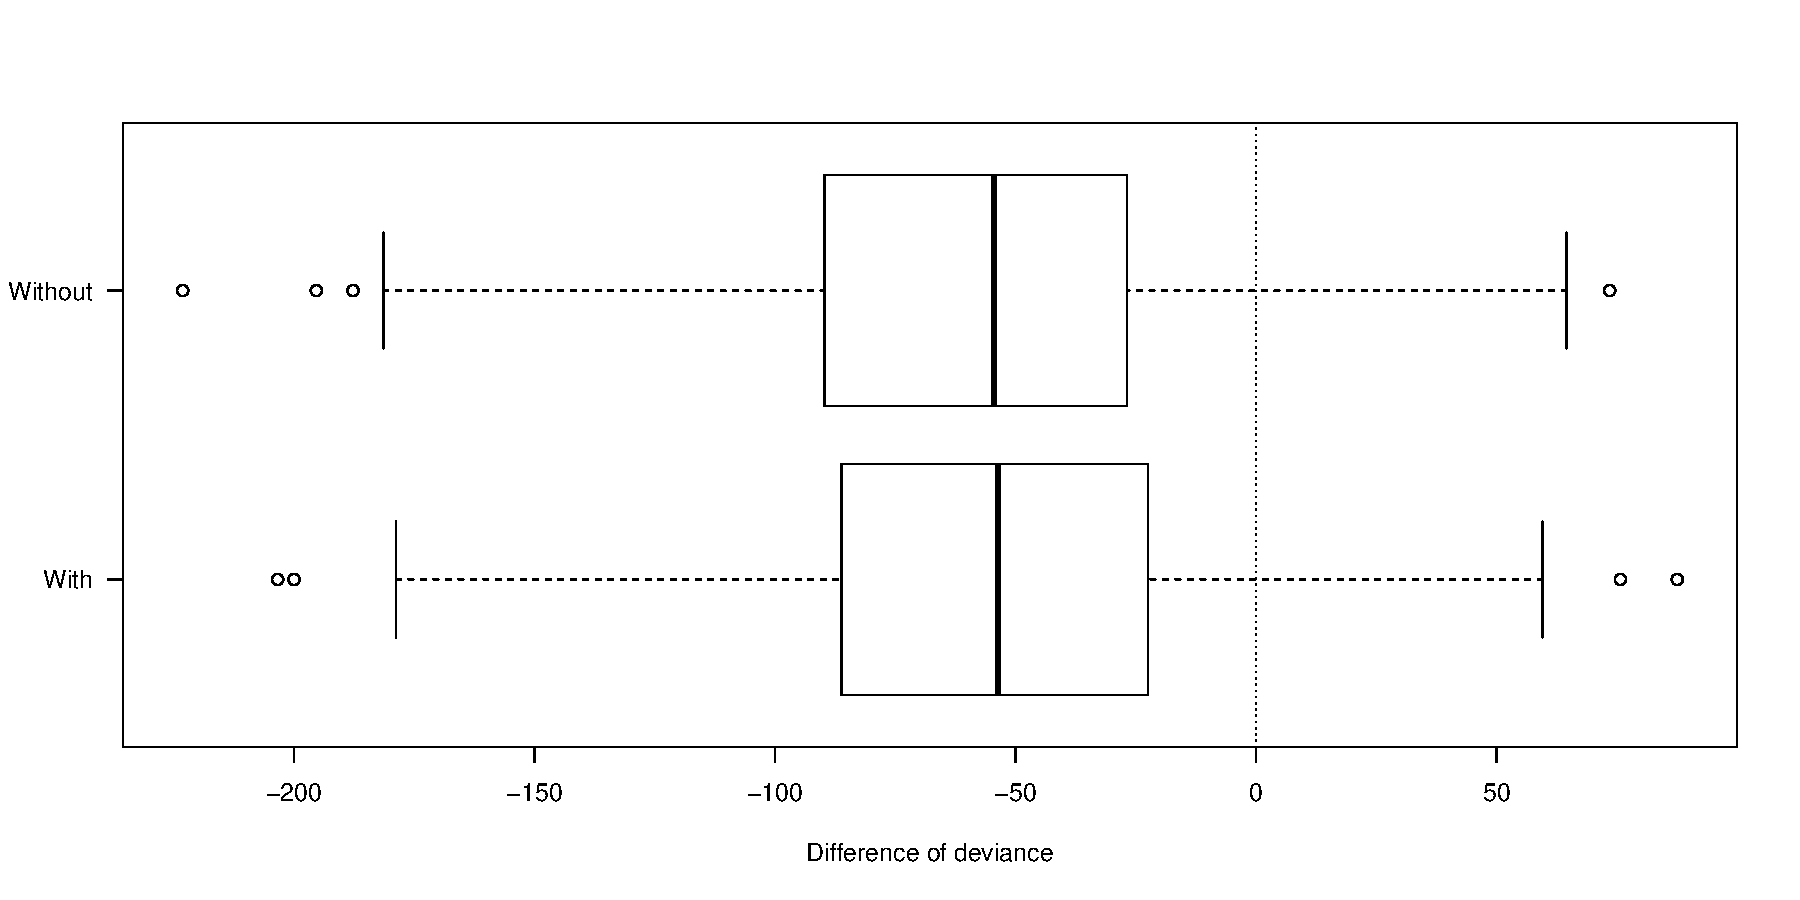
\includegraphics[scale=0.4]{deviances_simulation_correlated.pdf}
\end{figure}


\begin{table}
\caption{Difference of deviance results for FHTBoost, correlated case}
\label{table:uncorrelated-deviance}
\centering
\begin{tabular}{l|rr}
\toprule
& Updating & Fixed \\
\hline
Mean               &  -57.8  &  -58.8  \\
Standard deviation &   47.2  &   46.1  \\
Minimum            & -203.4  & -223.1  \\
Maximum            &   87.6  &   73.5  \\
\bottomrule
\end{tabular}
\end{table}


\subsubsection{Variable selection}
We now consider the variable selection metrics.
We first look at the covariate vector $\bbeta$, which affects the initial level $y_0$, and which is related to ``genomic'' variables.
The fixed intercept version is slightly better with regards to sensitivity, with a mean of 0.204 versus a mean of 0.157 for the changing intercept version.
So selecting informative variables,
This does come at the cost of a higher false discovery rate, with a mean as high as 0.652.
Here the changing intercept version has a mean of 0.439.
The specificity score is almost perfect in both cases.

We now consider the ``clinical'' covariates, used in $\bgamma$ and related to the drift $\mu$.
The changing intercept version performs quite a lot worse here than the fixed intercept version, overall.
It achieves a mean sensitivity of 0.273, while the fixed intercept version achieves 0.625.
However, the changing intercept then achieves a mean of 0.831 for specificity, where the fixed intercept version attains 0.537.
For the false discovery rate, the fixed intercept has a slightly higher mean, at 0.507, whereas the changing intercept version has a mean of 0.454.

For this scenario, as well, we see that the fixed intercept version has a higher optimal iteration number.
The mean $\mstop$ is 50 with a fixed intercept, compared to a mean of 19.5 for the changing intercept version.
Again this necessarily means that more variables are selected, and that coefficients from the changing intercept version will be more shrunken.

\begin{table}
\caption{High dimensional (genomic) part: Performance of FHTBoost in terms of variable selection, correlated case}
\label{table:correlated-y0}
\centering
\begin{tabular}{l|cc|cc}
\toprule
& Updating & & Fixed & \\
& Mean & Standard error & Mean & Standard error \\
\hline
Sensitivity & 0.157 & (0.084) & 0.204 & (0.081) \\
Specificity & 0.999 & (0.000) & 0.998 & (0.001) \\
FDR         & 0.439 & (0.218) & 0.652 & (0.181) \\
\bottomrule
\end{tabular}
\end{table}

\begin{table}
\caption{Low dimensional (clinical) part: Performance of FHTBoost in terms of variable selection, correlated case}
\label{table:correlated-mu}
\centering
\begin{tabular}{l|cc|cc}
\toprule
& Updating & & Fixed & \\
& Mean & Standard error & Mean & Standard error \\
\hline
Sensitivity & 0.273 & (0.187) & 0.625 & (0.245) \\
Specificity & 0.831 & (0.139) & 0.537 & (0.236) \\
FDR         & 0.454 & (0.250) & 0.507 & (0.130) \\
\bottomrule
\end{tabular}
\end{table}

\begin{table}
\caption{Optimal iteration number $\mstop$ results for FHTBoost, correlated case}
\label{table:correlated-mstop}
\centering
\begin{tabular}{l|rr}
\toprule
& Updating & Fixed \\
\hline
Mean               &  20.0  &  51.1  \\
Standard deviation &  12.1  &  24.4  \\
Minimum            &     2  &     2  \\
Maximum            &    65  &   148  \\
\bottomrule
\end{tabular}
\end{table}

\subsubsection{Conclusion}
In conclusion, while the fixed intercept version also here selects more true positive variables, it comes at a cost of selecting more false positives.
If we use the deviance to assess which one is best, then the fixed intercept version is the better one here as well.

\section{Discussion}
In general, we see that FHTBoost is able to estimate FHT models which achieve good performance, on data generated from a true FHT mechanism.
The performance achieved is especially high for the uncorrelated scenario.
As we have discussed, the variable selection has trade offs.
The fixed intercept version selects more true positives, but it also selects more false positives.
It does seem to be worth it, in the end, since it achieves a better generalization error in the form of a lower difference of deviance.
The results are also good in the highly correlated scenario.
Since this is a much more realistic scenario, we should give more weight to the results attained in it.
If so, it is difficult to make a conclusive statement on which version is better, as the results are very similar in the highly correlated scenario.
However, to narrow down the scope of the analysis in the next chapter, we will decide to only use the fixed intercept version, as we at least cannot say that it is not better than the changing intercept version.

    \chapter{Application on real data}
In the simulation we contrasted fixed/updating intercept versions, and in general, both FHTBoost seems to provide a decent model for correlated, realistic survival data, with average deviance much smaller than 0.

\todo[inline]{Make this paragraph better (merge)}

To truly be applicable in biomedical settings, we must see if the algorithm manages to achieve predictive power in a real study.
In this chapter, we consider data from \citet{oberthuer-data}, consisting of data from patients diagnosed with neuroblastoma.
The data consists of a small number of patients, with information on two covariates and around 10 000 gene expressions.
We use FHTBoost on this data and assess its performance.
We also compare the predictive power of our method to Cox regression, specifically CoxBoost, a version of Cox which has been adapted to a boosting framework (see, e.g., \citet{BinderSchumacher2008}), i.e., much like FHTBoost.

\section{Neuroblastoma}
We consider survival data from \citet{oberthuer-data}, consisting of patients diagnosed with neuroblastoma.
Neuroblastoma is a malignant pediatric tumor that accounts for about 8\% of all childhood cancers.
One of the hallmarks of the disease is its contrasting biological behavior, which results in diverse clinical courses ranging from spontaneous regression to rapid and fatal tumor progression despite intensive treatment.

In recent years, several markers have been reported to offer valuable prognostic information.
These markers are routinely determined by the current German neuroblastoma clinical trial NB2004 to stratify patients into groups of high risk (50\%)or low risk (50\%) of disease.
Therapeutic strategies vary according to these risk categories and range from a wait-and-see approach for those in the low risk group,
to intensive treatment for the high-risk group. Still, common clinical experience suggests that such risk classification is still suboptimal for a substantial number of patients.
The individual courses within these risk groups, in particular those of high-risk patients, still vary clearly.

Originally, the data consists of two separate data sets:
A larger training set, collected from Germany, and a smaller test set, collected from several countries.
The training set consists of 256 patients of the German Neuroblastoma Trials NB90-NB2004, where the patients were diagnosed between 1989 and 2004.
%Patients' age at diagnosis ranged from 0 to 296 months, with a median age at 15 months.
%Median follow-up for patients without fatal events was 4.5 years, with a range from 0.8 to 15.6 years.
The test set is an independent set of 120 patients from centers in several countries (including Germany).
In this set, 29 of the samples were obtained from German patients enrolled in German neuroblastoma trials, while the remaining samples are from patients enrolled in national trials in other countries.
%Here the age of patients at diagnosis ranged from 0 to 125 months, with a median at 15 months.
%For patients without fatal events, the median follow-up time was 4.4 years, and ranged from 0.4 to 18.1 years.

Due to few events in the NB2004 low risk group, and following \citet{bovelstad2009}, we merge the ``training set'' and the ``test set'' into one data set.
Hence, in total, the data consists of 362 patients suffering from neuroblastoma.
There are 9978 gene expressions measurements, comprised of those measurements which are in probes from both the ``training set'' and the ``test set.''
From each patient, we have information on their risk group according to the current German neuroblastoma trial as well as the possibly censored survival time.
This survival time was defined as time from diagnosis to first recurrence, and was censored at 5 years.
%Median follow-up time for the patients are 3.8 years.
In addition to the aforementioned risk group, the patient's age at diagnosis is recorded, resulting in two clinical covariates per patient.
89 out of the 362 observations have a missing age.
We remove all of these observations, and are left with a data set of 273.
So $N=273$.
Of these 273, 86 children were classified as having high-risk, while the remaining 187 were not.
It is coded as a binary variable, where both low risk and intermediate risk are coded as 0, and high risk as 1.
42 of the 273 children experienced a recurrence within the follow up, a proportion of 31.5\%.

%\begin{figure}
%\caption{Scatterplot of age in the dataset from \citet{oberthuer-data}.}
%\label{fig:age-scatter}
%\centering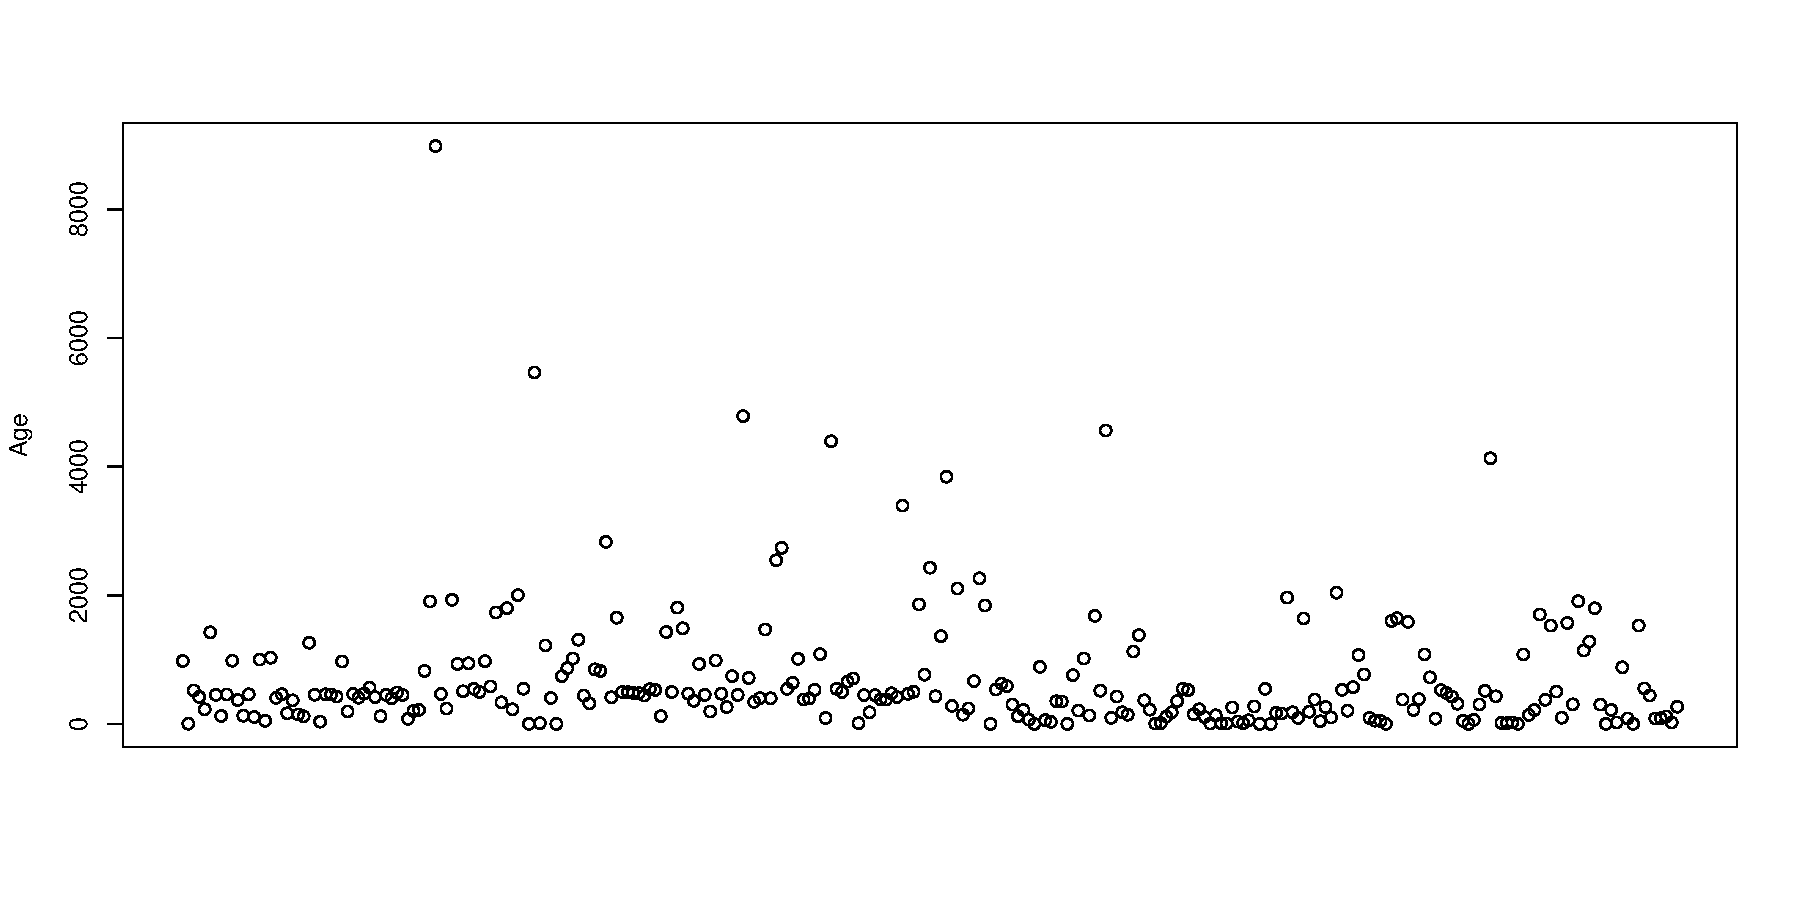
\includegraphics[scale=0.4]{age_scatter.pdf}
%\end{figure}

Due to the lack of data, \citet{bovelstad2009} generated 50 random splits of training and test sets from the merged data set.
We do the same, and generate 100 random splits times.
First, however, we report the analyses of one single (the first) split of train and test data, to give an example of how to interpret the results.

\section{Single split}
We standardize the data to ensure FHTBoost works.
The data are then split in a training set (2/3) and test set (1/3), stratified by the event status.
The training set consists of 182 patients, where 28 are observed events.
The test set consists of 91, where 14 are observed events.

\subsection{Cross-validation on training set}
As has been shown previously, cross-validation should be repeated with different division of folds, as this reduces variance in the estimate of $\mstop$.
We perform a (10 times) repeated 5-fold cross validation to find the optimal number of iterations.
Note in Figure \ref{fig:neuroblastoma-cv} the impact of running the 5-fold cross-validation in a repeated fashion:
Had we used a single 5-fold cross-validation, we would have selected different $\mstop$.
Had either of these been a s the optimal $\mstop$ is different between these different runs.
We first performed a 10-fold repeated cross-validation, but this parameter search did not converge, i.e., the log-likelihood kept increasing.
Upon further inspection, we found that one of the folds was the main cause of this, as the log-likelihood for that particular fold continued to increase, even after 400 iterations, while the other folds were in overfitting territory.
We concluded that splitting a training set of around 180 into 10 folds would eventually cause a problem in one of the folds, as there was too little information left.
We find $\mstop=20$ to be optimal in this case, as shown in Figure \ref{fig:neuroblastoma-cv}.
Each dotted gray line is the sum of the negative log-likelihood of a model trained on 4 folds and applied to the last fold, as a function of iteration number.
The solid black line is the mean of these 10 gray lines, and the red vertical line indicates the optimal $\mstop$, i.e., the minimizing iteration number.

\begin{figure}
\caption{Repeated 5-fold cross validation on training set generated from neuroblastoma data set \citep{oberthuer-data}.}
\label{fig:neuroblastoma-cv}
\centering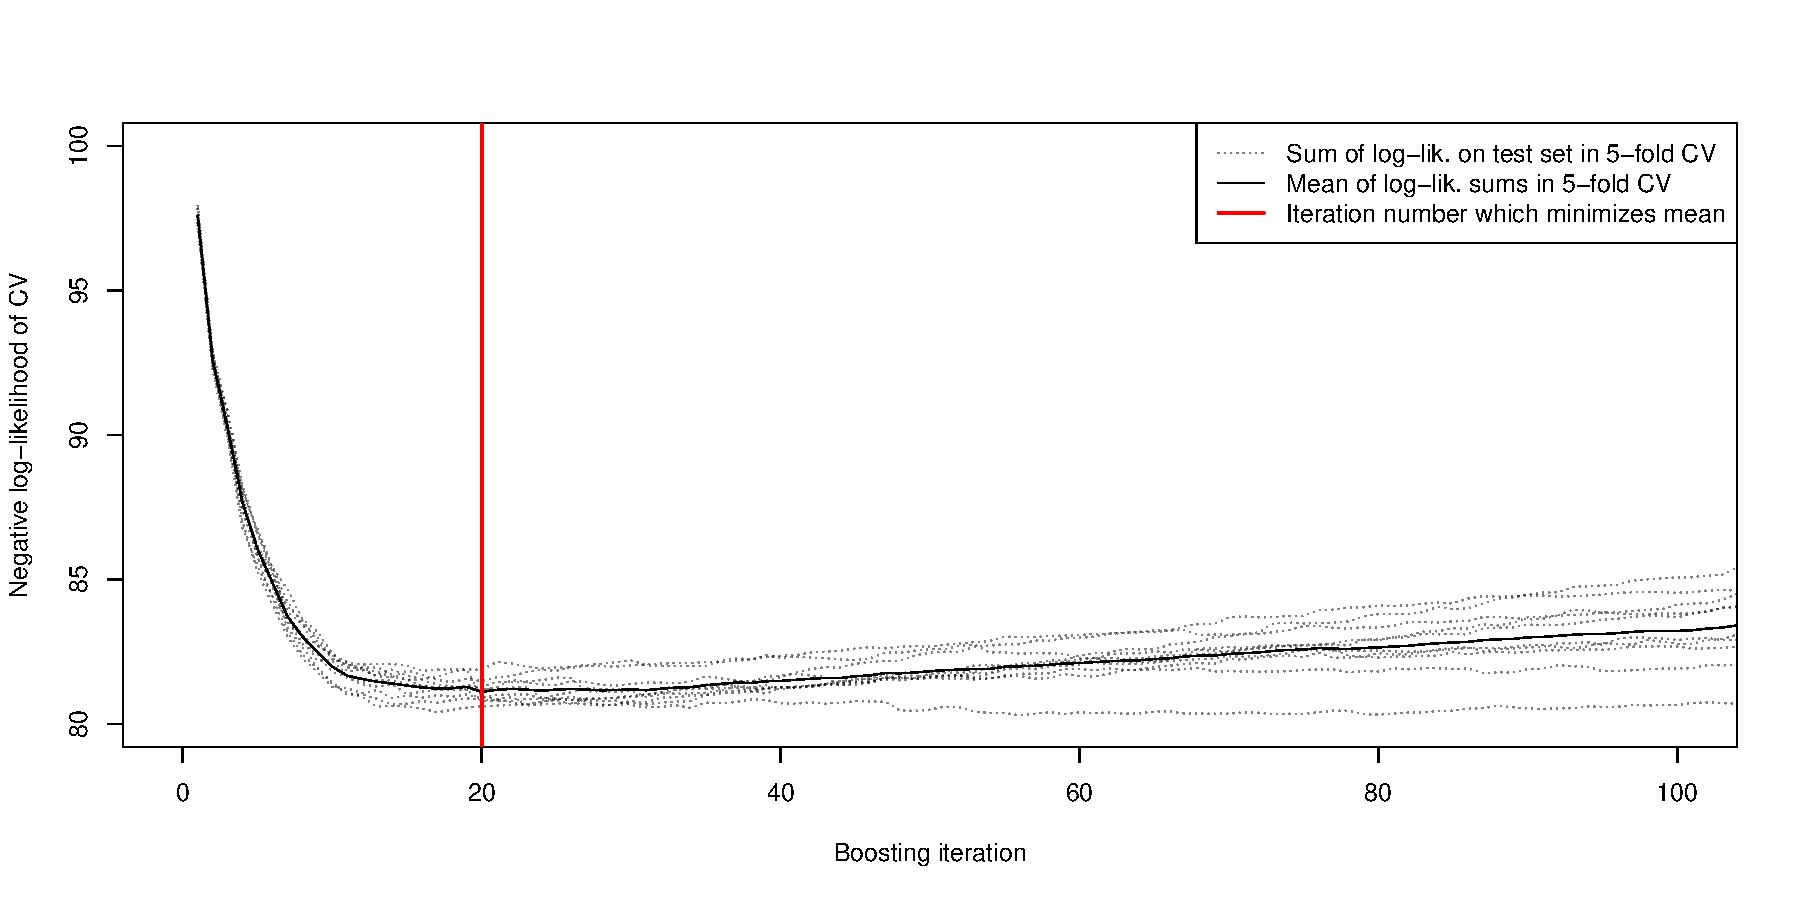
\includegraphics[scale=0.4]{example_cv_loglik.pdf}
\end{figure}

\subsection{Results}
We run the boosting algorithm with $\mstop$ iterations, to estimate the model parameters on the entire training set.

\begin{table}
\caption{Estimated null model on neuroblastoma \citep{oberthuer-data}}
\label{tab:neuroblastoma-intercepts}
\centering
\begin{tabular}{lr}
\toprule
  & Value\\
\hline
$\beta_0$ & 0.692 \\
$\gamma_0$ & 0.077 \\
\bottomrule
\end{tabular}
\end{table}

\subsubsection{Baseline, null model, interpretation}
We first look at the intercepts, reported in Table \ref{tab:neuroblastoma-intercepts}, meaning, the null model parameters.
The estimated intercept for the gene data, $\beta_0$, is 0.692.
We recall that in the FHT model, the vector $\bbeta$ corresponds to the initial level $y_0$ of the health process, with the log link function.
The null model, without any covariate effects, therefore has a $y_0$ of $\exp(0.692)=1.998$.
Further, the intercept for the clinical data is estimated to be 0.077.
This means that the health process with the FHT interpretation that arises from our estimation is a Wiener process with a relatively small initial level of 1.998, and with a \textit{positive} drift, albeit slightly, of 0.077.
Recall also that the Wiener process has a unit variance in each time unit, meaning the variance is equal to the time unit $t$.
The large variability of the process relative to its starting point means there is still a significant chance of recurrence of neuroblastoma.
The resulting health process is
\begin{equation*}
    Y(t)=1.998+W(t)\cdot0.077t,
\end{equation*}
where $W(t)\sim N(0,\sqrt{t})$,
i.e.,
\begin{equation*}
    Y(t)\sim N(1.998+0.077t,\sqrt{t}).
\end{equation*}
To get a feeling of the variability of it, and potential trajectories of such a process, we plot 10 realizations of this process in Figure \ref{fig:neuroblastoma-wien}.
Of these particular 10 processes, 8 processes at some point go below 0.
In the FHT interpretation, then, these health processes would cause a death, or, a recurrence of the neuroblastoma cancer.
To get a better estimate of the proportion of health processes not dying, we need to sample more processes.
We sampled 10000, and 6221 of these went below 0 within $t=40$, i.e., a proportion of 0.378 did not experience recurrence.
In section \ref{sec:FHT}, specifically in equation \eqref{eq:P-inf-FHT}, we stated the probability of an IG FHT lifetime not ending, i.e., the cure rate.
We will have a non-zero cure rate if the drift is positive, like we have here in our null model.
We calculate this for our estimated null model, obtaining
\begin{align*}
    \Pr{(T=\infty)}=1-\Pr{(T<\infty)}&=1-\exp{(-2\cdot y_0^{[0]}\cdot\mu^{[0]})}\\
    &=1-\exp{(-2\cdot 1.998\cdot 0.077)}=0.265,
\end{align*}
meaning about three in four should have a recurrence during their lifetime.
For this training set, 28 out of 182 are observed events, meaning only 0.154 have experienced a recurrence.
Note that this is with a medium follow-up of 4.5 years.
It is, however, still a bit off from the cure rate obtained from the estimated null model, but our model does predict a non-zero proportion of long-term survivors, which is good.
\begin{figure}
\caption{Wiener processes with parameters $y_0=1.998$ and $\mu=0.077$, corresponding to the estimated null model from the neuroblastoma data set \citep{oberthuer-data}.}
\label{fig:neuroblastoma-wien}
\centering
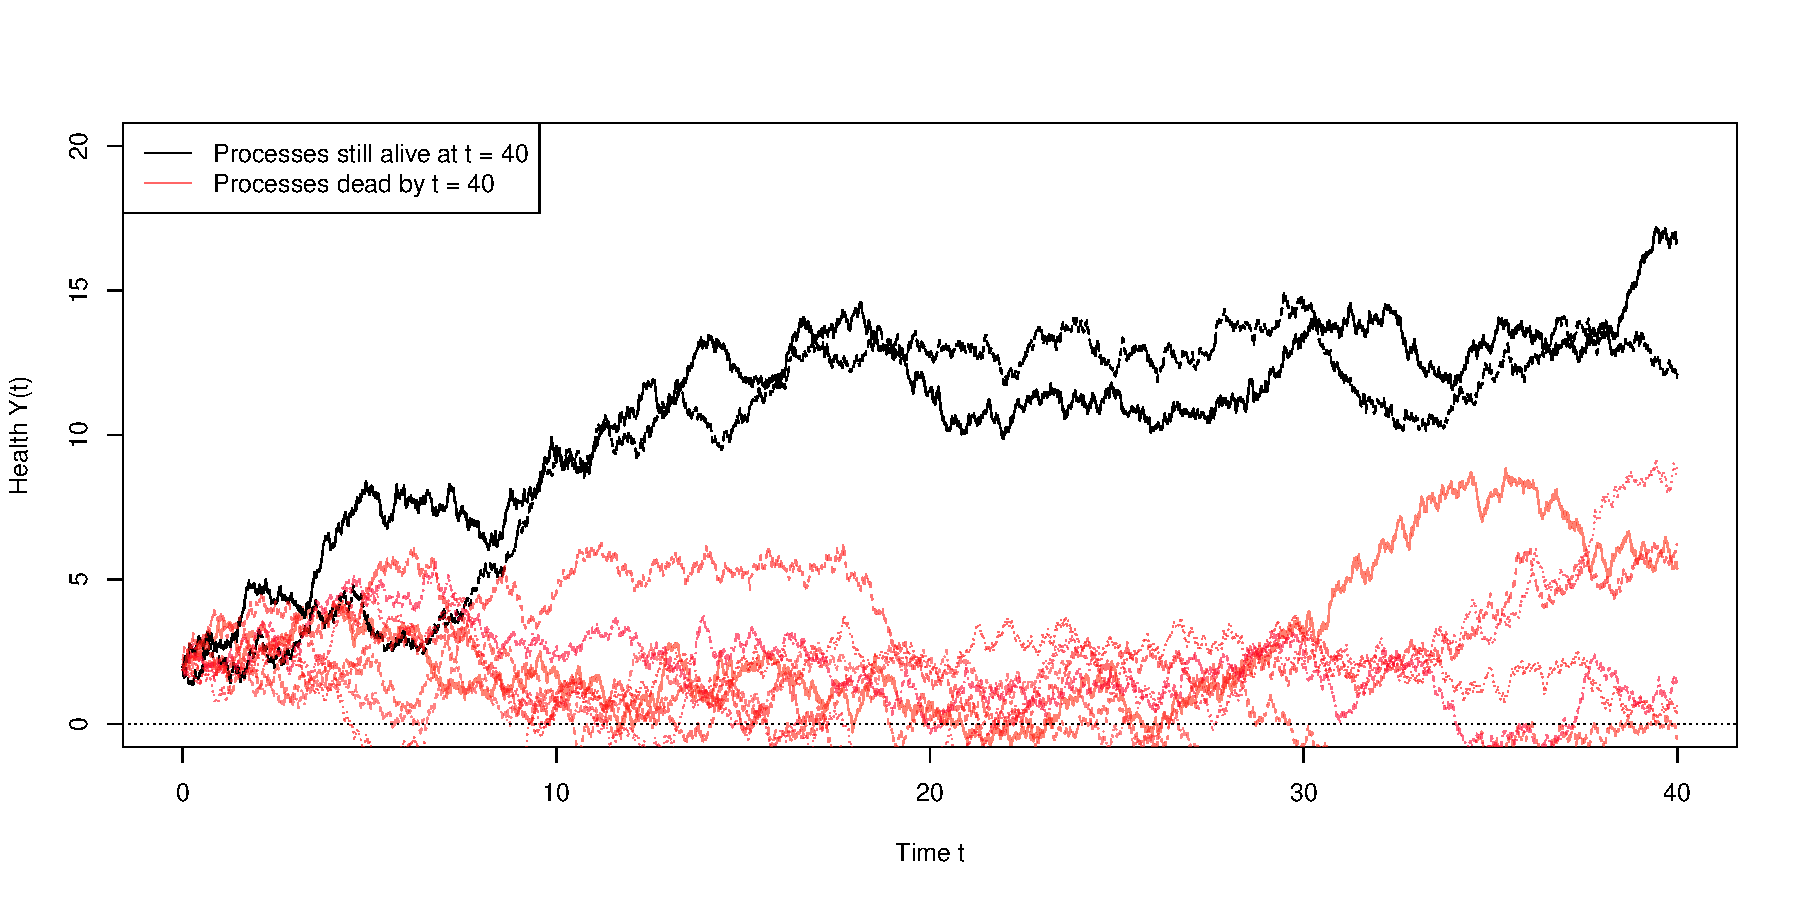
\includegraphics[scale=0.4]{example_wieners.pdf}
\end{figure}

Consider the fact that the initial level $y_0$ is quite low.
Since we are looking at when, if ever, a neuroblastoma patient will have a recurrence after a surgery, this initial level of the Wiener process is the health level of a patient at surgery.
The health of such a child is often presumable quite precarious, as neuroblastoma is a malignant cancer.
Therefore it makes sense that the initial level $y_0$ is quite low.
However, the survival probability of patients vary, as is experienced by clinicians, even among those specified as high-risk.
Most children will, as estimated by our model, survive.

Now consider the fact that the drift $\mu$ is positive.
Since the individuals in the study are young children, and we are looking at a timeframe that does not comprise the length of a typical human life, the health level of most children should indeed increase after the surgery.

\subsubsection{Estimated covariates}
Let us further look at estimated covariate effects (Table \ref{tab:oberthuer-beta} and Table \ref{tab:oberthuer-gamma})
We see that the boosting algorithm has included both covariates into the model.
Before splitting into training and test sets, we centered and scaled each column of the covariate matrices, such that the mean across all individuals is (approximately) 0 for each covariate $j$,
%\begin{equation}
%    \overline{x}_j=\frac{1}{n}\sum_{i=1}^n x_{i,j}\approx 0,
%\end{equation}
and the standard error is approximately 1.
%\begin{equation}
%    s_j=\frac{1}{n}\sum_{i=1}^n (x_{i,j}-\overline{x}_j)^2\approx 1.
%\end{equation}
%(See a previous section for an explanation of why centering and scaling is important.)
For the gene expressions, this is not particularly important with regards to interpretation, as the scale of these do not lend themselves easily to interpretation.
However, to properly consider the interpretation of the estimated parameters corresponding to the clinical measurements, we should
scale these back to their original scale.
For example, the covariate corresponding to risk, namely $\gamma_1$, is originally either 0 or 1, depending on the covariate.
After standardizing, these are -0.677 and 1.472, respectively.
The most striking result here is the large parameter corresponding to risk.
We calculate the drift parameter for those individuals designated as high-risk, and it is
\begin{equation*}
    \mu^{[0]}_{\text{high-risk}}=0.077-0.189\cdot1.472=-0.202.
\end{equation*}
Whereas for those designated as low and intermediate risk, it is
\begin{equation*}
    \mu^{[0]}_{\text{low-risk}}=0.077-0.189\cdot-0.677=0.205.
\end{equation*}
Since age is standardized, these two drift covariates should be the mean drift parameters for each of the groups.
The effect of age is negative, which means that there is some downward effect on the drift as the child's age increases.
This negative effect could also potentially lead to low-risk individuals having an estimated negative drift, if the child is sufficiently old.
This is, however, not the case.
The effect of age is so small as to not impact the sign of the drift.
Because the maximum standardized age is 4.193, the age contribution to drift is bounded below by 
\begin{equation*}
    -0.029\cdot4.193=-0.122.
\end{equation*}
Similarly, there are no high-risk individuals for which the drift will be positive, since the minimum standardized age is -0.724, and so the effect of age is bounded above by
\begin{equation*}
    -0.029\cdot0.724=0.021.
\end{equation*}
Hence, crucially, this means that the model predicts that all high-risk individuals will eventually have a recurrence of neuroblastoma cancer.
This seems to resonate with the fact that these children are indeed characterized as having a high risk of recurrence.
Those not designated as high-risk, on the other hand, have a probability of not experiencing recurrence, using the formula seen previously, namely
\begin{equation*}
    1-\exp{(-2\cdot y_{0}^{[0]}\cdot\mu_{\text{low-risk}}^{[0]})}=1-\exp{(-2\cdot 1.998\cdot 0.205)}=0.559.
\end{equation*}
We should therefore expect, based on the estimated model, that more than half of the low-risk patients should recover.


\begin{table}
\caption{Results of estimated gene coefficients on neuroblastoma data \citep{oberthuer-data}.}
\label{tab:oberthuer-beta}
\centering
\begin{tabular}{lrr}
\toprule
Gene $j$      & $\beta_j$ (full) & $\beta_j$ (genomic only)\\
\hline
Gene 49   & -0.010  &      0  \\
Gene 1447 & -0.069  & -0.047  \\
Gene 3191 &      0  & -0.051  \\
Gene 2442 &  0.012  &      0  \\
Gene 4447 &      0  & -0.062  \\
Gene 5307 &      0  &      0  \\
Gene 5527 & -0.073  & -0.098  \\
Gene 5725 & -0.009  &      0  \\
Gene 6532 & -0.011  &      0  \\
Gene 6701 &  0.015  &      0  \\
Gene 6901 &  0.011  &      0  \\
\bottomrule
\end{tabular}
\end{table}

\begin{table}
\caption{Results of estimated clinical coefficients on neuroblastoma data \citep{oberthuer-data}.}
\label{tab:oberthuer-gamma}
\centering
\begin{tabular}{lrr}
\toprule
Clinical covariate & $\gamma_j$ (full) & $\gamma_j$ (clinical only)\\
\hline
Risk      &  -0.189  &  -0.268\\
Age       &  -0.029  &       0 \\
\bottomrule
\end{tabular}
\end{table}

We observe that 8 genes have been selected in 20 boosting iterations (see Table \ref{tab:oberthuer-beta}).
Some effects are estimated to be positive, some to be negative.
Again, the gene expression measurements have been centered and scaled.
However, a larger parameter does not necessarily mean that the effect of this gene is in general larger than others, as that still depends on the distribution of these.
It is more difficult here to say how much the genomic data helps in explaining the variance.


\subsection{Difference of deviance on the test set}
The test set consists of 91 individuals, of which 14 have experienced recurrence.
With the estimated model, we calculate the deviance, as seen in Section \ref{sec:deviance}.
Recall that the performance of a model is good when the difference in deviance is small (i.e. negative with a large absolute value).
We obtain a difference of deviance on -95.2, which is quite a lot!

\section{Comparing a clinical-genetic model to clinical-only and genetic-only models}
\citet{bovelstad2009} analysed the neuroblastoma data and compared different ways of combining clinical and genomic data in Cox models.
As mentioned in subsection \ref{subsec:FHT-combine}, the FHT model lends itself easily to combining genomic and clinical data.
Our boosting method FHTBoost offers a simple way to combine clinical and genetic data in estimating.
There is also a straightforward way to only use clinical covariates, or to only use genetic covariates.
To do this, we can use the cyclical version of the algorithm, where we booth both parameters in each step, but they have their own tuning parameter.
This lets us fix the number of boosting steps of the parameter not to be boosted to 0.
In other words, a genomic version of FHTBoost, or $y_0$-only version of FHTBoost, where we boost only the initial level $y_0$.
This version of FHTBoost has $m_{\text{stop},1}$, corresponding to $\mu$, fixed at 0, while we perform cross-validation in the usual way to find the optimal $m_{\text{stop},2}$, corresponding to $y_0$.
Similarly, the clinical version fixes $m_{\text{stop},2}$ at 0, and tunes the other, $m_{\text{stop},1}$, corresponding to $\mu$.
In this way, we can compare the performance of our model across the genetic and clinical data, in a similar way as in \citet{bovelstad2009}.

We do the estimation and the test set calculation, and we get the difference of deviance results shown in table \ref{tab:deviances}.
We see here, in fact, that in this case the full model is beaten by the genomic model, with difference of deviance of -95.2 and -104.4, respectively.

\begin{table}
\caption{Difference of deviance results.}
\label{tab:deviances}
\centering
\begin{tabular}{cc}
\toprule
Boosting type & Difference of deviance \\
\hline
Full & -95.2 \\
Clinical ($y_0$) only  & -14.5 \\
Genetic ($\mu$) only & -104.4 \\
\bottomrule
\end{tabular}
\end{table}

Furthermore, we calculate the Brier scores at the time points of the test set.
See Figure \ref{fig:brier-FHT} for a comparison of the Brier score of the three different FHT models.
We see here that, in fact, the genomic model performs best, and quite strikingly so.

\begin{figure}
\caption{Brier scores for FHT models.}
\label{fig:brier-FHT}
\centering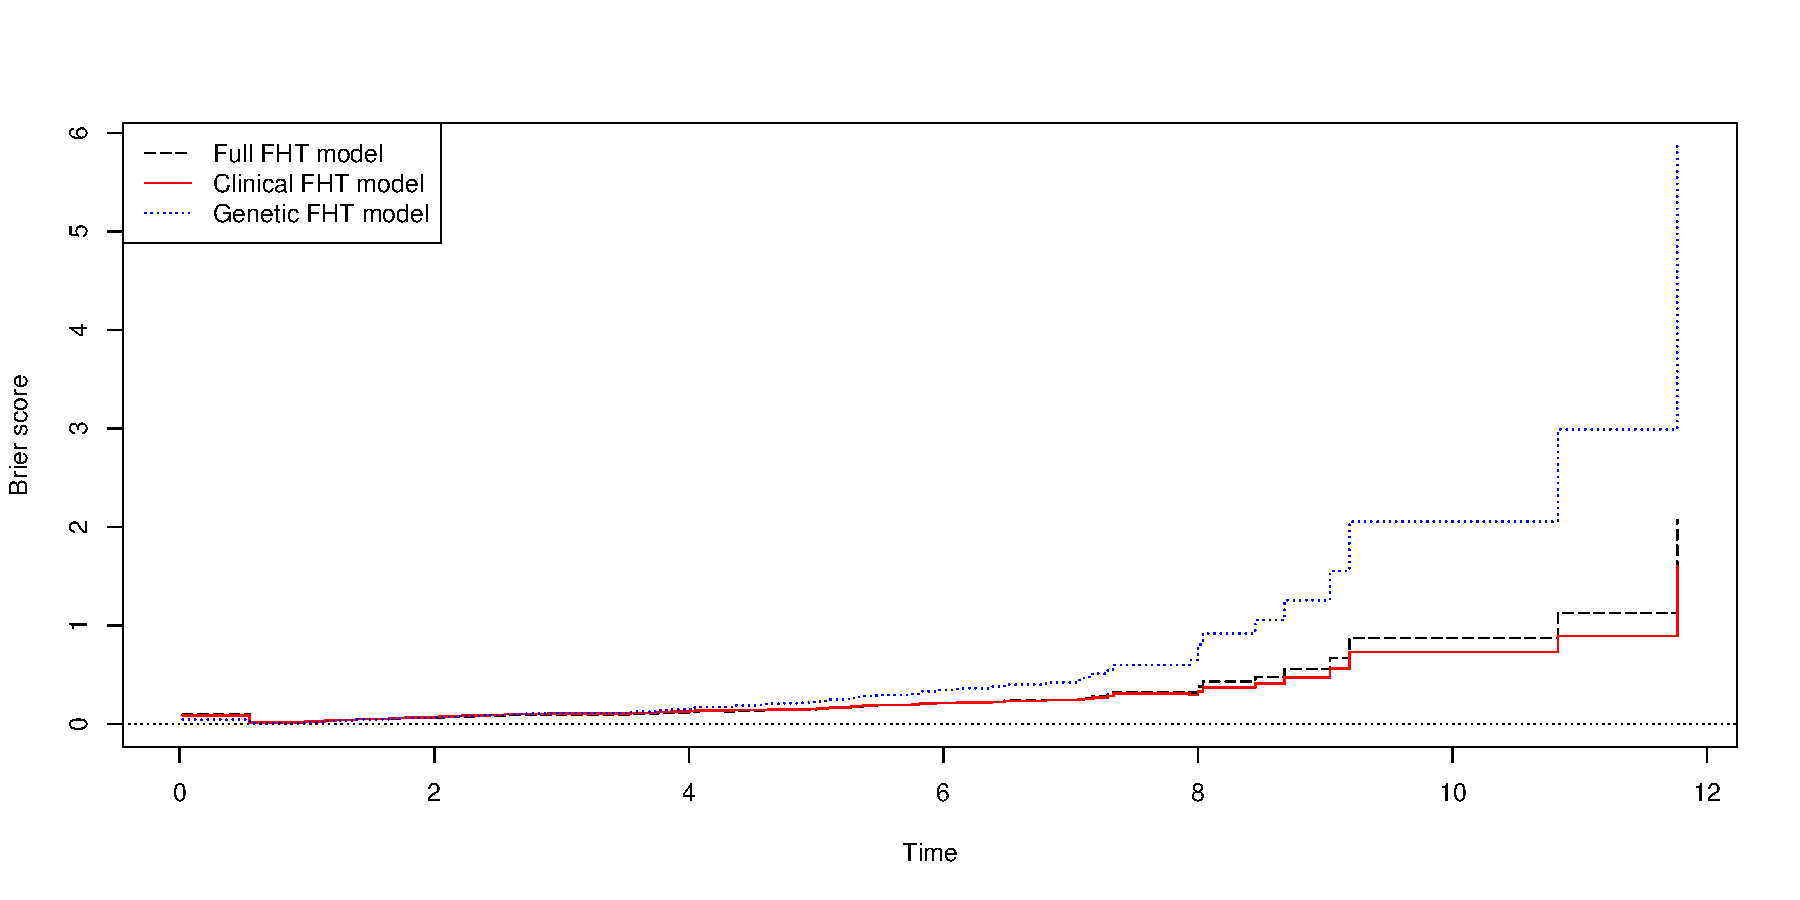
\includegraphics[scale=0.4]{brier_FHT.pdf}
\end{figure}

\section{Comparison with the Cox model}
The Cox model which has been discussed previously, in Chapter 2.
We compared our model with the Cox model as implemented in CoxBoost \citep{...}, setting
\begin{equation}\label{eq:lambda-nu}
    \lambda=N\frac{1-\nu}{\nu},
\end{equation}
as suggested in \citet{DeBin2016}, where $N$ is the number of individuals in the data set on which the estimator is applied, and $\nu$ is the step length mentioned in the various boosting algorithms in chapter \ref{ch:boosting}, which we by convention always set to 0.1.

For the specific case discussed previously, we calculate the Brier score for these models.
Consider now a comparison between the Brier score for the full FHT model and the Cox model, in Figure \ref{fig:brier-cox-both}.
We can see that the Cox model performs better for all times, but the difference in performance also increases over time.
Consider now Figure \ref{fig:brier-cox-genetic}, in which we compare the Cox model to the genomic model.
What is especially interesting here is that the Brier score of the genomic model almost overlaps with the Brier score of the Cox model.
That is, except the positive jumps that the Cox model performs in the beginning, mostly from time 0 to 4.
I do not know why these jumps happen.

\begin{figure}
\caption{Brier scores for Cox and both.}
\label{fig:brier-cox-both}
\centering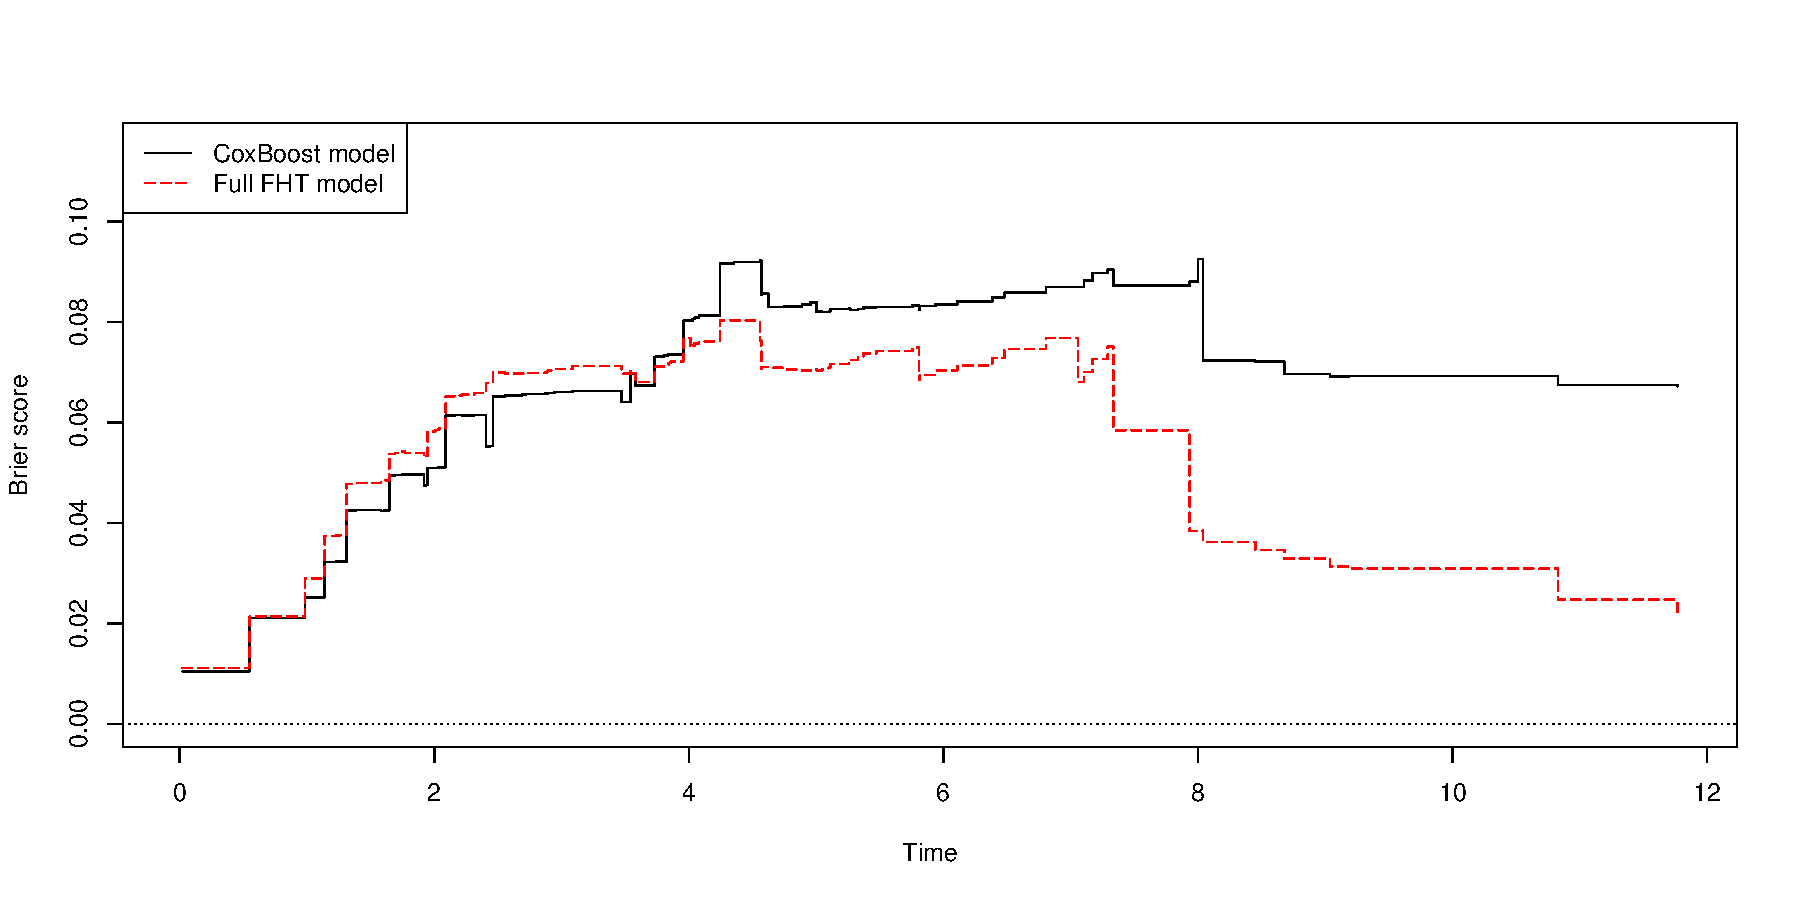
\includegraphics[scale=0.4]{brier_cox_both.pdf}
\end{figure}
See Figure \ref{fig:brier-cox-both} for a comparison of the Brier score of the boosted Cox model and the boosted FHT model.
\begin{figure}
\caption{Brier scores for Cox and genetic FHT model.}
\label{fig:brier-cox-genetic}
\centering
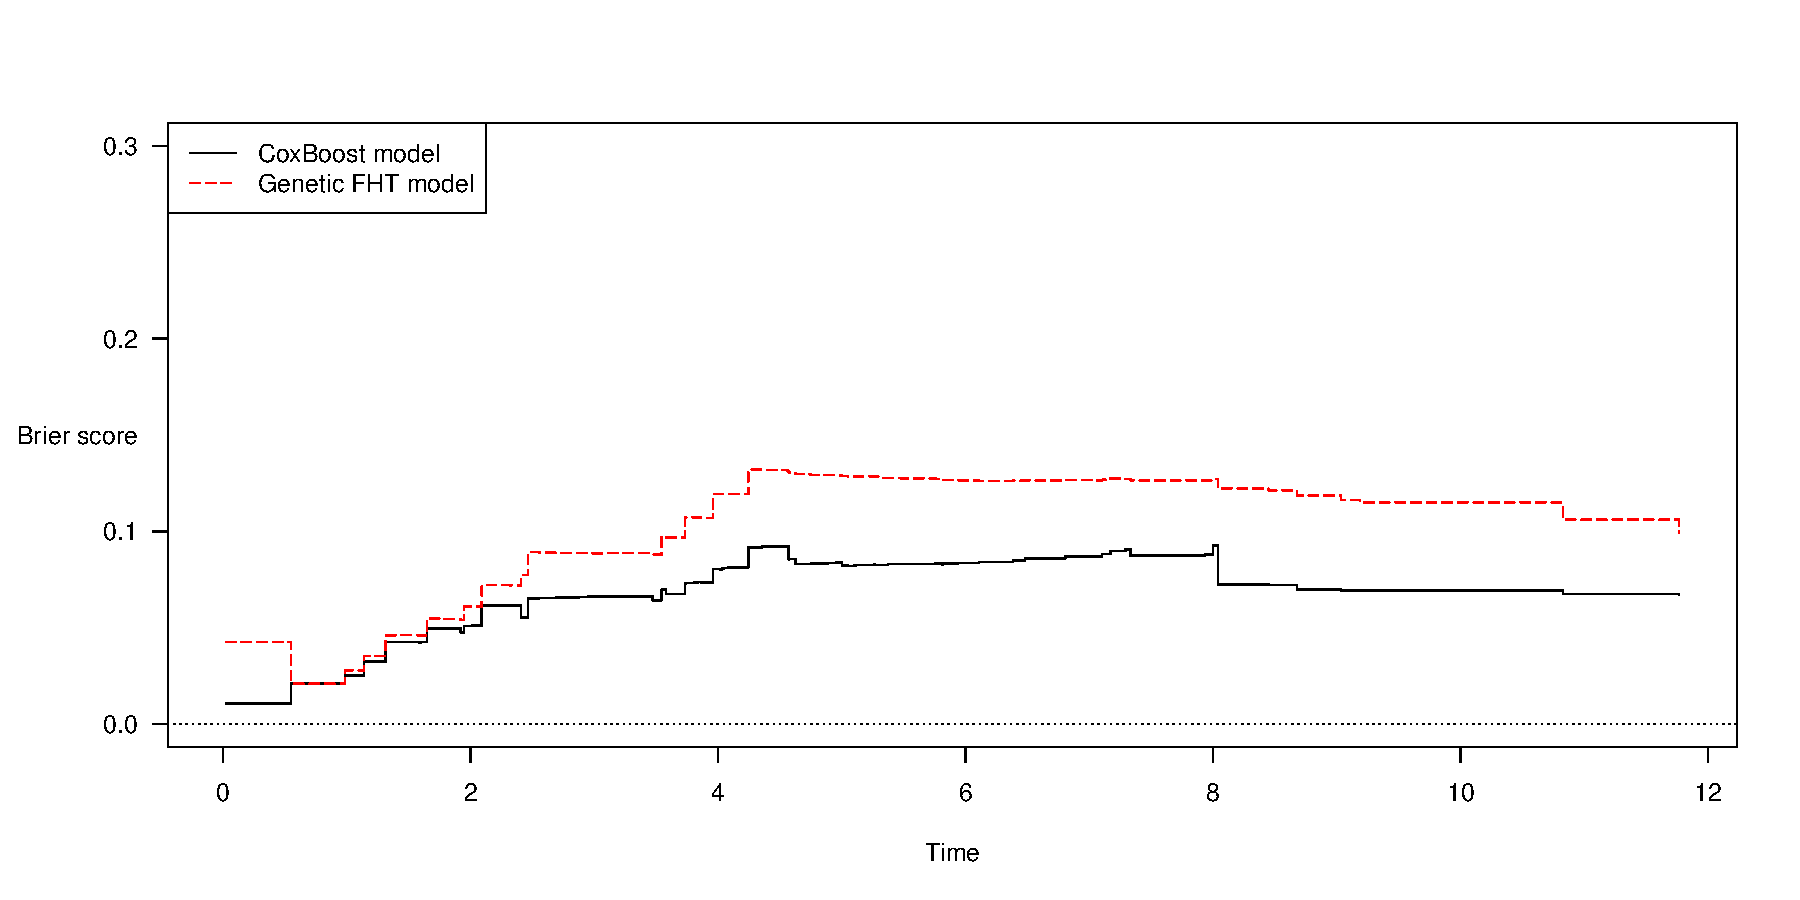
\includegraphics[scale=0.4]{brier_cox_genetic.pdf}
\end{figure}

%\begin{figure}
%\caption{Brier scores for Cox and Cox mandatory model.}
%\label{fig:brier-cox-mandatory}
%\centering
%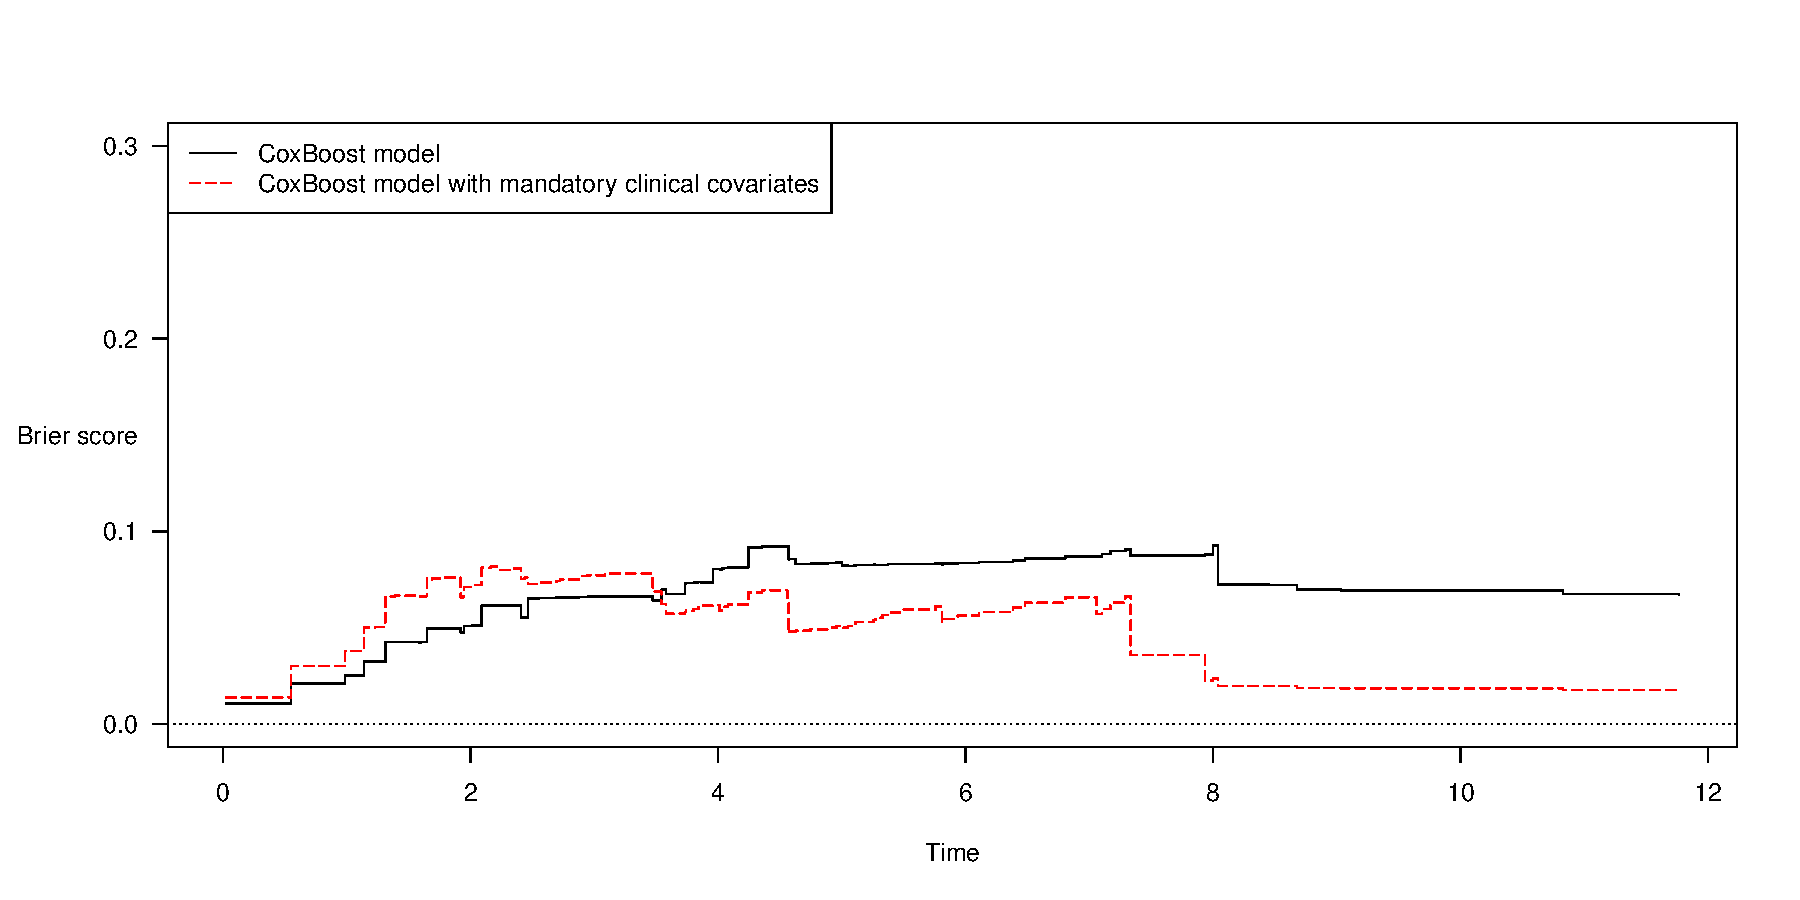
\includegraphics[scale=0.4]{brier_cox_mandatory.pdf}
%\end{figure}

%\todo[inline]{Cite these packages! I think cite(package) in R}


\section{Analysis of 100 train/test splits}
\citet{bovelstad2009} generated 50 random splits of training and test sets from the data, to see the distribution.
We now generate 100 splits of training and test sets, in the same manner.
We use the same method as above.
We first estimate parameters based on the training set, and then calculate the model's difference of deviance, on the test set, using the parameters estimated on the training set.

\subsection{Comparing deviance of FHT models}
We now consider the difference of deviance across all 100 splits of training and test sets.
All 
The 
See Figure \ref{fig:neuroblastoma-deviances} for difference of deviance boxplot.
We use the median of difference of deviance as the main measure of interest.
It is -24.3172 for the full model, and -21.60033 for the clinical model, and 4.009162 for the genomic model.
See Figure \ref{fig:neuroblastoma-deviances} for a boxplot of these.

\begin{figure}
\caption{Boxplot for difference in deviance for different variants of the FHT model.}
\label{fig:neuroblastoma-deviances}
\centering
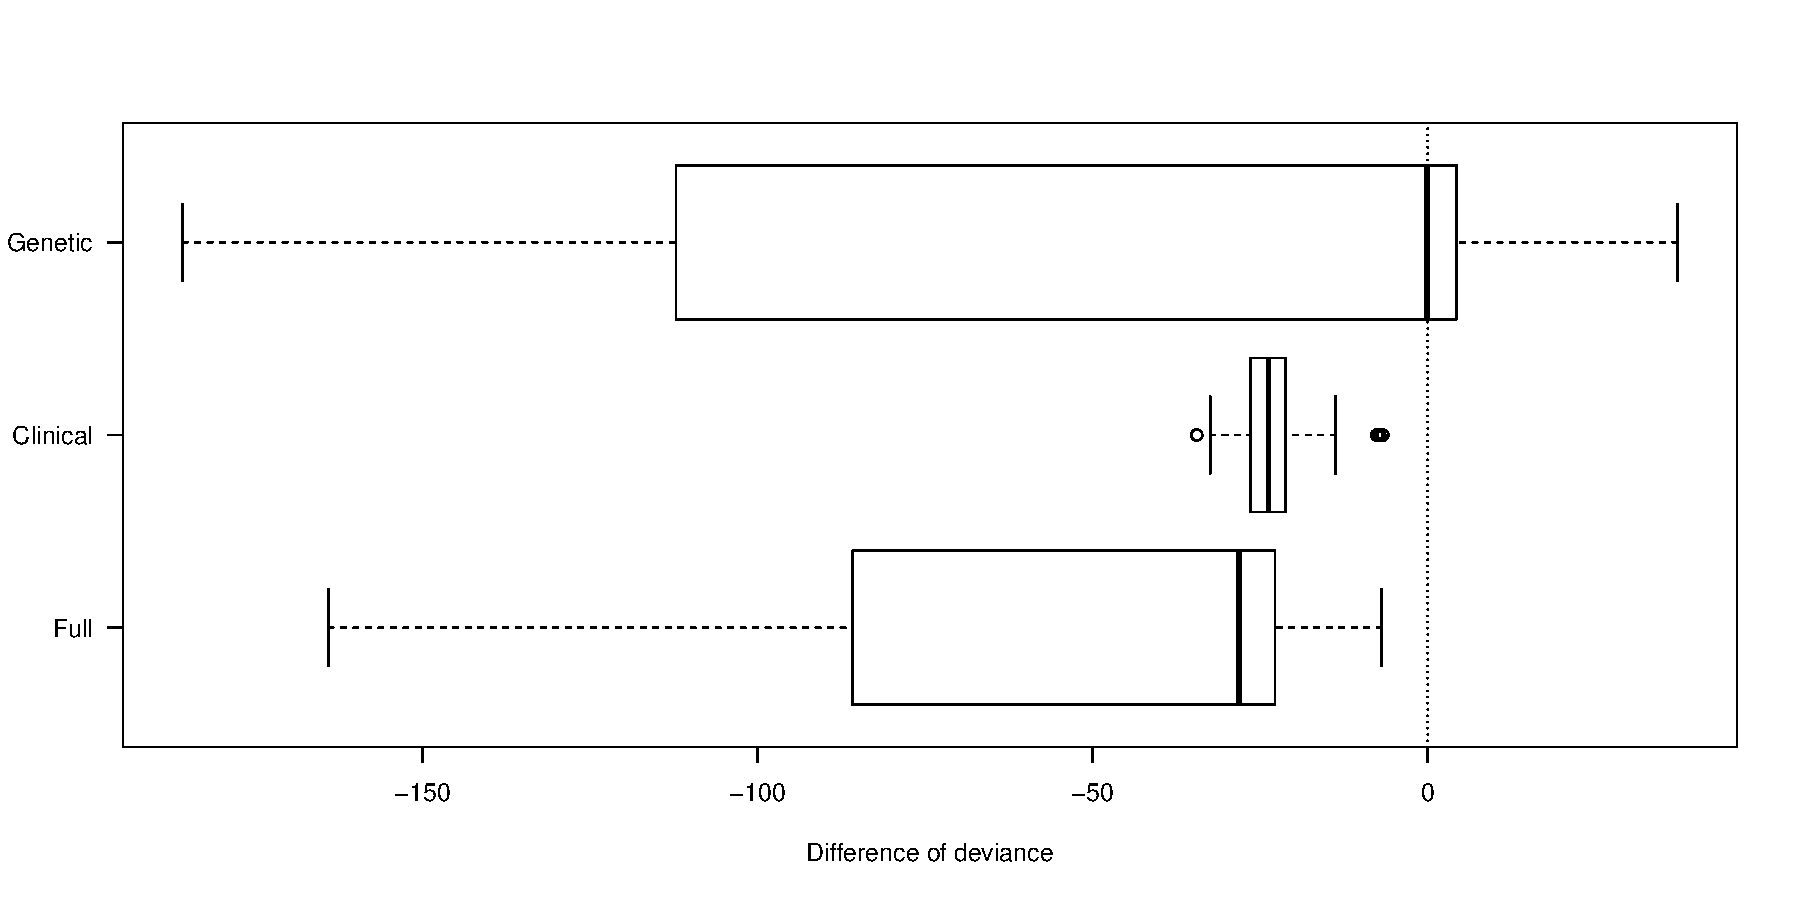
\includegraphics[scale=0.4]{deviance_FHT.pdf}
\end{figure}

These deviances look a bit strange, at least the box for the full model, and the box for the genomic model.
The median looks to be very strangely positioned, all the way to the right of the boxes.
We plot histograms of these two to consider why.
See Figure \ref {fig:neuroblastoma-deviances-histo}.
The reason turns out to be that they are quite bimodal in their distribution.
Both have large peaks around 0, and both have smaller and wider peaks more to the left.
We see that the full model consistently improves performance with covariates, i.e., has a negative difference of deviance.
This resonates with the fact that the clinical model also improves over the null model.
However, the genomic model very often does not improve on the null model.
Although, its most extreme values are in cases where the difference of deviance is very small, and so these are cases where the genomic model outperforms the full model.

\begin{figure}
\caption{Histogram of difference of deviance for the genomic model and the full model.}
\label{fig:neuroblastoma-deviances-histo}
\centering
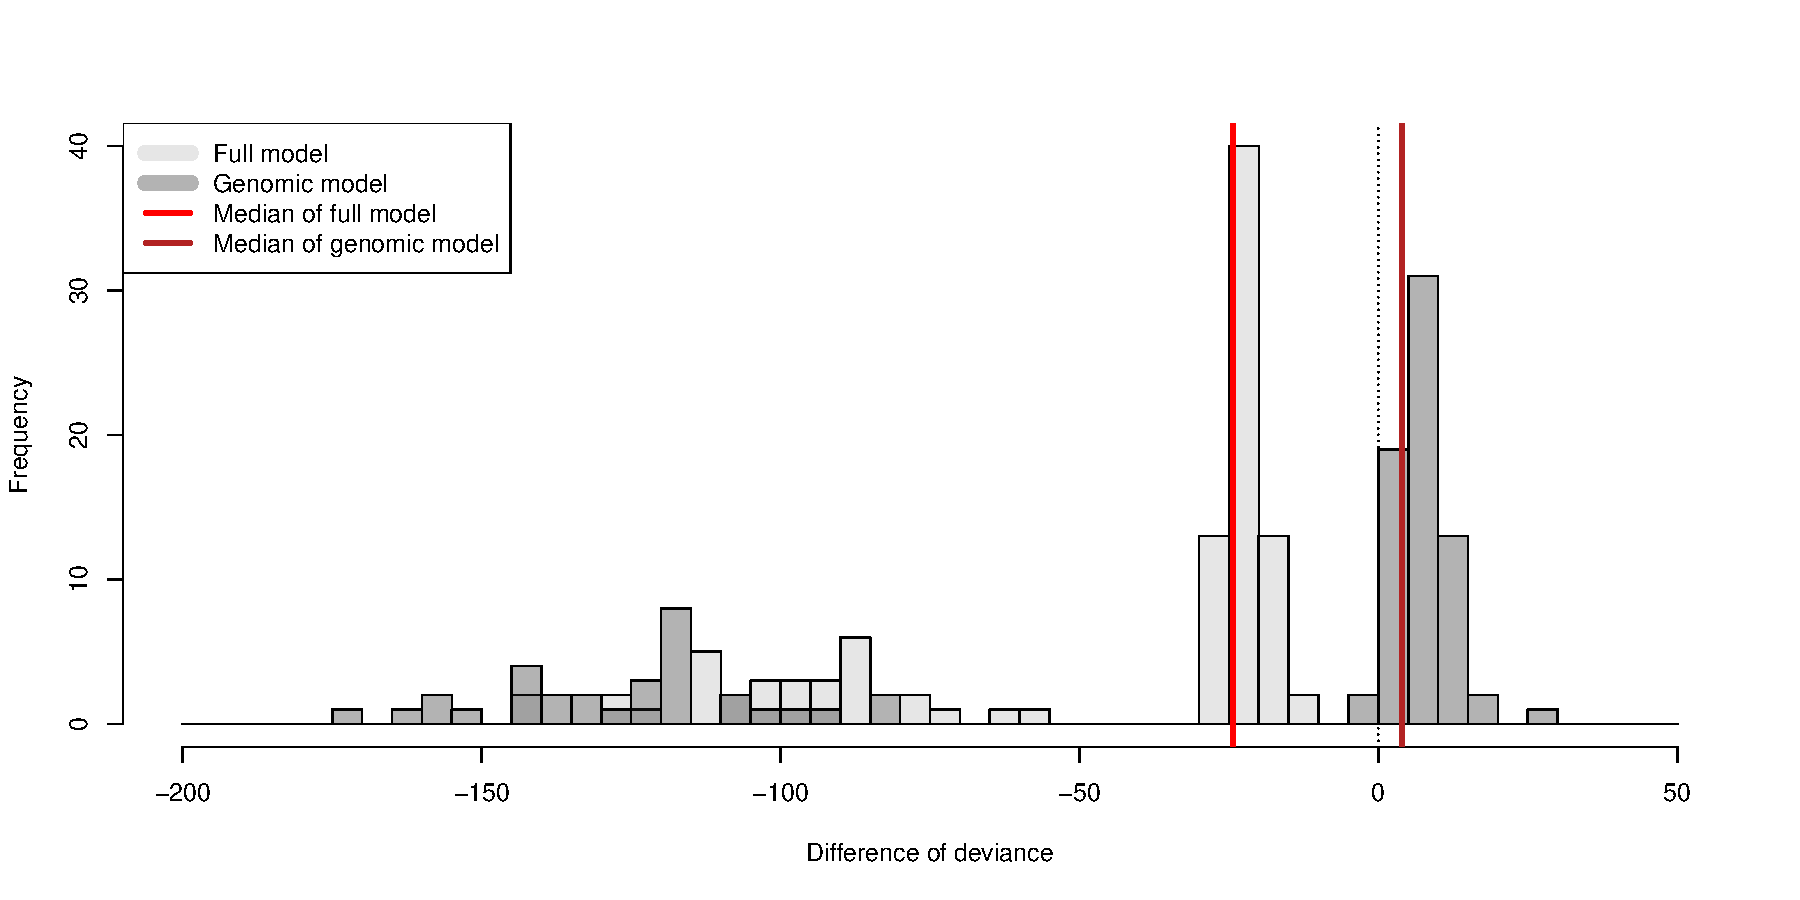
\includegraphics[scale=0.4]{deviances_histogram.pdf}
\end{figure}


\subsection{Integrated Brier scores results}
We now calculate integrated Brier scores for all 100 splits.
A boxplot can be seen in Figure \ref{fig:neuroblastoma-integrated-brier}.
\begin{figure}
\caption{Boxplot of integrated Brier scores.}
\label{fig:neuroblastoma-integrated-brier}
\centering
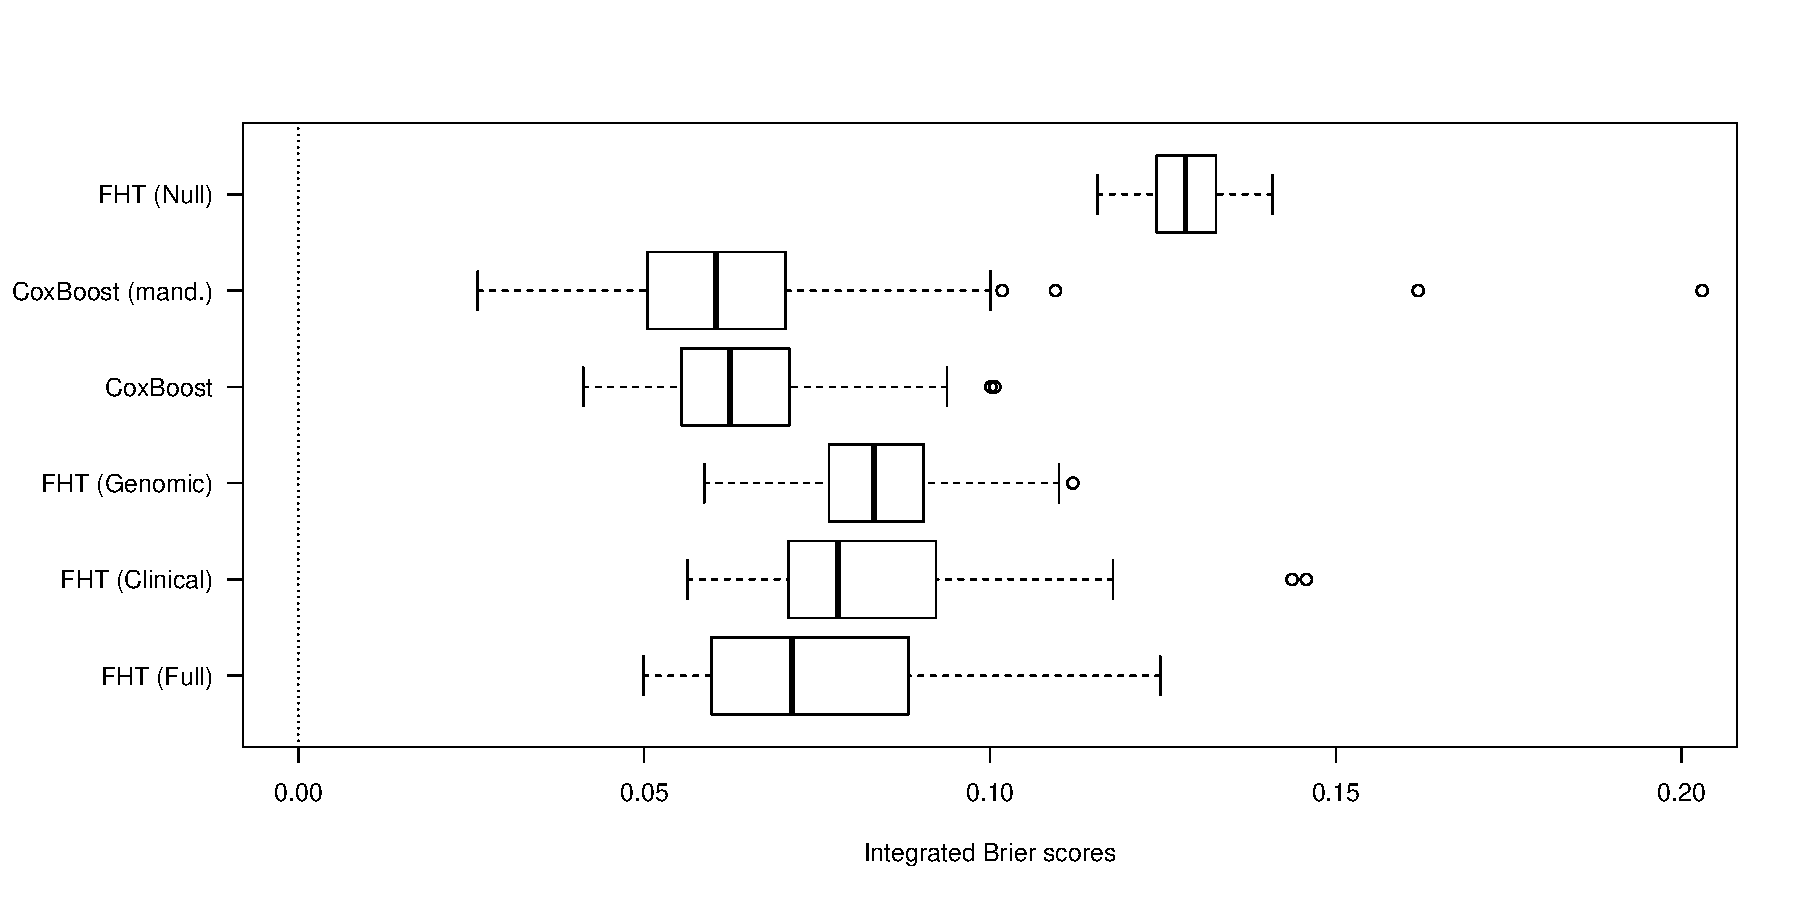
\includegraphics[scale=0.4]{integrated_brier_boxplot.pdf}
\end{figure}
With regard to this integrated Brier score, the full model performs slightly better than the clinical model.
It turns out that the full model performs slightly better than the clinical model, based on the median difference of deviance.
It might therefore appear as if the genomic data sometimes improves performance, and sometimes does not.
However, the genomic-only model vastly outperforms the full FHT model.
We get a median integrated Brier score of 3.9 for the full FHT model, only slightly beating the clinical one at 3.7.
The genomic model, however, achieves 6.8, whereas the Cox model performs best, at 7.7.

I'm not sure why this happens, especially since the log-likelihood of the full model is best.
It looks like the observations which improve the likelihood are not those which improve the Brier score.
If these were the same, then we would most likely see the same model perform best in both regards.
It might, for example, be, at least based on the example seen earlier, that the genomic model in this case better explains the later observations, whereas the clinical data is better at lifetimes of smaller value.

\section{Conclusion}
Applying the FHT model to this data set has been a partly fruitful effort.
The model is able to incorporate covariate information to improve the model fit.
However, the predictive power is quite off from the Cox model.

%\section{Colon cancer}
%We now consider data originating from \citet{marisa-data}, consisting of patients diagnosed with colon cancer.
%Colon cancer is the third most common cancer, and the fourth leading cause of cancer death worldwide \citep{marisa-data}.
%Pathological staging is the only prognostic

%The French national CIT program involves a multicenter cohort of 750 patients with stage I to IV CC.

%About the data.

%We remove observations where any covariate is missing.

%We have four clinical measurements.
%These are sex, which is coded as a dummy variable $x_{\text{sex}}\in\{-1,1\}$, age, subtype, and finally stage.

%In the original data set, some survival times are originally 0.
%We first tried setting these to $10^{-9}$, but it resulted in numerical instability when using numerical optimization to find the maximum likelihood intercepts.
%We then tried setting these successively to $10^{-9},\,10^{-8},\,\cdot$, and not until 0.1 did we achieve numerical stability.
%Note that this likely has a large effect on the estimated parameters.

    \chapter{Discussion and future work}
\label{sec:discussion}
In this thesis, we have looked at problems in survival data, and specifically first hitting time models.
While Cox regression is by far the most popular method used to estimate survival data models, it has shortcomings that we have discussed.
One of them is the fact that it relies on a proportional hazards assumption, which does not hold in a variable selection setting, which is almost always the case when we perform regression with high-dimensional data.
The Cox model does still, however, work well in practice, and has good predictive power.
First hitting time (FHT) models are flexible alternatives that do not rely on the proportional hazards assumption.
As of the time of writing for this thesis, no methods for FHT models exist to estimate parameters in a high-dimensional setting.
We have therefore discussed ways of estimating models that work well in such a setting.
In particular, we have discussed gradient boosting \citep{friedman2001}, both methods for estimating one parameter, and extensions to several parameters.

Our goal with the thesis work was therefore to combine FHT models and gradient boosting.
To this goal, we have developed an algorithm for fitting an FHT model with linear additive predictors.
The estimation algorithm works as follows.
It starts by initializing the additive predictors to intercepts, specifically the intercepts that maximize the log-likelihood of the training set.
We then perform iterations where we in each step include a regularized linear least squares function in \textit{one} of the covariates and \textit{one} of the parameters, namely the combination of covariate and parameter which leads to the largest increase in the log-likelihood function.
The algorithm was implemented from scratch as a package which we called \textit{FHTBoost}, and it is freely available for download at \verb|https://github.com/vegarsti/fhtboost|.
It can be installed directly in R by using a command in the DevTools R package \citep{devtools} called \verb|install_github|, namely \verb|install_github("vegarsti/fhtboost")|.

In the boosting algorithm, we used component-wise linear learners without intercepts.
We developed two versions of FHTBoost, one with a fixed intercept, and one where the intercept is treated as a nuisance parameter, and is optimized in each iteration until the boosting is stopped.
In a simulation study, we found that both versions manage to select informative variables and shrink parameter sizes, and, importantly, increase model fit while doing so.
In an uncorrelated scenario, the fixed intercept version achieves markedly better deviance on a test set.
However in a correlated and realistic scenario, the two versions achieve very similar performance.
In all cases, the mean deviance is well below zero.
To limit the scope of the analysis, we chose to use only the fixed intercept version in the next section, which looked at a neuroblastoma data set \citep{oberthuer-data}, which is a realistic data set consisting of measurements of 9978 genes and two clinical covariates.
When used on this data set, FHTBoost always estimates a model where covariates increase the log-likelihood of the model, on a test set, meaning the model fit is better than in the case of no covariates.
The models estimated with FHTBoost have good predictive power, achieving a mean Brier score of 0.074.
The mean for the regular Cox model is 0.064, while for a mandatory version of Cox, which did not penalize the clinical covariates, the mean was 0.069.
In other words, the FHTBoost model achieves comparable predictive power as state of the art Cox models, but init did not outperform it.

There are several interesting directions for further work.
One is to apply \textit{FHTBoost} on other real-life high-dimensional survival data sets.
This would allow for a broader assessment of its usefulness and predictive power on real-life problems.
One of the strengths of gradient boosting is that it is easy to use in combination with different component-wise base learners.
In this thesis, we have only considered linear base learners.
It would be interesting to include nonlinearity into these, which could be done by e.g. using regularized splines of one dimension as base learners.
Another interesting direction of further work would be to incorporate the FHT model into the existing ecosystem of gradient boosting packages in R.
This ecosystem is based on the package \textit{mboost} \citep{mboost}.
The framework used for FHT regression fits into the GAMLSS framework.
It should therefore be possible to use the \textit{gamboostLSS} \citep{gamboostlss-paper, gamboostLSS-manual} package.
There also exists an extension for fitting GAMLSS models to censored data, \textit{gamboostLSS.cens} \citep{gamlsscens}.
It should be possible to include our parameterization of the inverse Gaussian here.
By including our inverse Gaussian parameterization with its log-likelihood and derivatives, it should be possible to use the entire library of base learners in \textit{mboost}.


    \appendix           % "Chapter" is renamed "Appendix"
    \appendixpage       % Similar to \part*{Appendices}, but appears in TOC.

    \chapter{Appendix 1: Differentiating the IG FHT}
First we have the likelihood,
\begin{align}\label{eq:fht-loglik}
\begin{split}
L(\btheta)&=\prod_{i=1}^n\p*{\frac{y_0}{\sqrt{2\pi\sigma^2\ti^3}}\exp\left[-\frac{(y_0+\mu \ti)^2}{2\sigma^2\ti}\right]}^{\di}\\
&\times\sqb*{1-\Phi\p*{-\frac{y_0+\mu \ti}{\sqrt{\sigma^2\ti}}}-\exp\p*{-\frac{2y_0\mu}{\sigma^2}}\Phi\p*{\frac{\mu \ti-y_0}{\sqrt{\sigma^2\ti}}}}^{1-\di},
\end{split}
\end{align}
with respect to parameters $\mu$, and $y_0$. First, note that for any cumulative distribution function $F$ that is symmetric around 0, and for $x\in\R$,
\begin{equation}
    F(x)=1-(1-F(x))=1-F(-x),
\end{equation}
and so in particular,
\begin{equation}
    \Phi(x)=1-(1-\Phi(x))=1-\Phi(-x),
\end{equation}
and thus we can rewrite \eqref{eq:fht-loglik} as
\begin{align}\label{eq:fht-loglik-proper}
\begin{split}
L(\btheta)&=\prod_{i=1}^n\p*{\frac{y_0}{\sqrt{2\pi\sigma^2\ti^3}}\exp\left[-\frac{(y_0+\mu \ti)^2}{2\sigma^2\ti}\right]}^{\di}\\
&\times\sqb*{\Phi\p*{\frac{y_0+\mu \ti}{\sqrt{\sigma^2\ti}}}-\exp\p*{-\frac{2y_0\mu}{\sigma^2}}\Phi\p*{\frac{\mu \ti-y_0}{\sqrt{\sigma^2\ti}}}}^{1-\di}.
\end{split}
\end{align}
It is easier to work with the log likelihood, so we take the log of \eqref{eq:fht-loglik-proper} and get
\begin{align}
\begin{split}
    l(\btheta)&=\sum_{i=1}^n\di\p*{\ln y_0-\frac{1}{2}\ln\p*{2\pi\sigma^2\ti^3}-\frac{\p*{y_0+\mu\ti}^2}{2\sigma^2\ti}} \\
    &+
    (1-\di)\ln\p*{\Phi\p*{\frac{\mu\ti+y_0}{\sqrt{\sigma^2\ti}}}-\exp\p*{-\frac{2y_0\mu}{\sigma^2}}\Phi\p*{\frac{\mu\ti-y_0}{\sqrt{\sigma^2\ti}}}}
\end{split}
\end{align}
To make things easier, let us introduce some intermediate functions here. Let
\begin{equation}
f_i(\btheta)=\ln y_0-\frac{1}{2}\ln\p*{2\pi\sigma^2\ti^3}-\frac{\p*{y_0+\mu\ti}^2}{2\sigma^2\ti}
\end{equation}
and
\begin{equation}
g_i(\btheta)=\Phi\p*{\frac{\mu\ti+y_0}{\sqrt{\sigma^2\ti}}}-\exp\p*{-\frac{2y_0\mu}{\sigma^2}}\Phi\p*{\frac{\mu\ti-y_0}{\sqrt{\sigma^2\ti}}}.
\end{equation}
Thus we see that the partial derivatives are
\begin{equation}
    \frac{\partial}{\partial y_0}l(\btheta)=\sum_{i=1}^n\di \frac{\partial}{\partial y_0}f_i(\btheta)+(1-\di)\frac{\frac{\partial}{\partial y_0}g_i(\btheta)}{g_i(\btheta)}
\end{equation}
and
\begin{equation}
    \frac{\partial}{\partial \mu}l(\btheta)=\sum_{i=1}^n\di \frac{\partial}{\partial \mu}f_i(\btheta)+(1-\di)\frac{\frac{\partial}{\partial \mu}g_i(\btheta)}{g_i(\btheta)}.
\end{equation}

\begin{align}
\begin{split}
    \frac{\partial}{\partial y_0}g_i(\btheta)&=\frac{1}{\sqrt{\sigma^2\ti}}\phi\p*{\frac{\mu\ti+y_0}{\sqrt{\sigma^2\ti}}}+\frac{2\mu}{\sigma^2}\exp\p*{-\frac{2y_0\mu}{\sigma^2}}\Phi\p*{\frac{\mu\ti-y_0}{\sqrt{\sigma^2\ti}}} \\
    &+
    \frac{1}{\sqrt{\sigma^2\ti}}\exp\p*{-\frac{2y_0\mu}{\sigma^2}}\phi\p*{\frac{\mu\ti-y_0}{\sqrt{\sigma^2\ti}}}
\end{split}
\end{align}


\begin{equation}
    \frac{\partial}{\partial y_0}f_i(\btheta)=\frac{1}{y_0}-\frac{y_0+\mu\ti}{\sigma^2\ti}
\end{equation}

\begin{equation}
    \frac{\partial}{\partial \mu}f_i(\btheta)=-\frac{y_0+\mu\ti}{\sigma^2}
\end{equation}

\begin{align}
\begin{split}
    \frac{\partial}{\partial \mu}g_i(\btheta)&=\frac{\ti}{\sqrt{\sigma^2\ti}}\phi\p*{\frac{\mu\ti+y_0}{\sqrt{\sigma^2\ti}}}+\frac{2y_0}{\sigma^2}\exp\p*{-\frac{2y_0\mu}{\sigma^2}}\Phi\p*{\frac{\mu\ti-y_0}{\sqrt{\sigma^2\ti}}} \\
    &-
    \frac{\ti}{\sqrt{\sigma^2\ti}}\exp\p*{-\frac{2y_0\mu}{\sigma^2}}\phi\p*{\frac{\mu\ti-y_0}{\sqrt{\sigma^2\ti}}}
\end{split}
\end{align}

    \chapter{Appendix 2: R code}\label{appendix2}

\section{Generate correlated gene and clinical data}
This code is by Riccardo de Bin, and as mentioned in section \ref{sec:generating-correlated-data}, it is written by him.
We add it here for the sake of transparency.

\label{code:generate-correlated-data}
\begin{lstlisting}
generate_clinical <- function(n.obs=200,tot.genes=10000,n.groups=100,n.clin=NULL,n.gene=NULL,mean.n.gene=15,
                        mu.g=6,sigma.g=0.65,mu.c=1,sigma.c=0.5,rho.c=0,rho.b=0,rho.g=0,phi=0.1,nu=10,tau=20) {
  # n.obs (integer) = number of observations
  # tot.genes (integer) = number of molecular predictors
  # n.groups (integer) = number of pathways (molecular predictors correlated to each other)
  # n.clin (vector) = number of clinical predictors for each group (if NULL, no clinical predictors are generated)
  # n.gene (vector) = number of molecular predictors for each group (if NULL, all the group sizes are generated randomly, if its length is smaller than n.groups the unspecified size are generated randomly as well)
  # mean.n.gene (integer) = average sizes of molecular predictors for group. Relevant only if n.gene is NULL or length(n.gene)<n.groups
  # mu.c (integer) = mean of the log-normal distribution of the clinical variables
  # sigma.c (integer) = standard deviation of the log-normal distribution of the clinical variables
  # mu.g (integer) = mean of the log-normal distribution of the genes
  # sigma.g (integer) = standard deviation of the log-normal distribution of the genes
  # rho.g (vector) = correlation within each block of genes (equal for all of them). Default (for all or only the part of the groups for which it is not specified) is 0.
  # rho.c (vector) = vector containing the correlation between the clinical predictors in each pathway
  # rho.b (vector) = vector containing the correlation between the clinical and the molecular predictors in each pathway
  # phi (integer) = standard deviation of the normal distribution modeling the multiplicative noise to the signal
  # nu (integer) = mean of the normal distribution modeling the additive noise to the signal
  # tau (integer) = standard deviation of the distribution modeling the additive noise to the signal

  require(mvtnorm)
  require(corpcor)

  if(tot.genes<n.groups) stop('The number of genes must be bigger than the number of pathways\n')
  # if the groups sizes are not provided, generate them
  length.n.gene<-length(n.gene)
  if(tot.genes<sum(n.gene)) stop('The number of genes must be bigger than the total number of genes in the pathways\n')
  {if(is.null(n.gene)) length.n.gene<-0
    else if (length.n.gene<n.groups) warning(paste0('The length of n.gene is smaller than ',n.groups,'. The sizes of the remaining groups is generated randomly\n'))}
  if (length.n.gene<n.groups)
  {
    n.gene<-c(n.gene,round(rnorm(n.groups-length.n.gene,mean.n.gene,0.3*mean.n.gene)))
    n.gene[n.gene<1]<-1 # to have no empty group
  }
  # update the number of groups generated
  sumBs<-sum(n.gene)
  # if we generate more genes than those indicated in tot.gene, tell how many genes are actually generated
  {if(sumBs>tot.genes)
  {
    tot.genes<-sumBS
    warnings(paste0('Total number of simulated genes equal to ',sumBS,'\n'))
  }
    else n.gene[n.groups+1]<-tot.genes-sumBs} # the last block contains all the genes not belonging to the first n.groups blocks
  # if the correlation among genes is not specified (for all or only part of the groups), we set it to 0
  if(length(rho.g)<n.groups) rho.g<-c(rho.g,rep(0,n.groups-length(rho.g)))

  # check for the clinical structure and complete the lists
  ifelse(is.null(n.clin),length.n.clin<-0,length.n.clin<-length(n.clin))
  # check if the number of clinical groups is reasonable
  if(length.n.clin>n.groups) {
    n.clin<-n.clin[1:n.groups]
    warnings(paste0('Number of clinical groups too large, only the first ',length.n.gene,' are used.\n'))
  }
  if (sum(rho.c) > 0) {
    n.clin[(length.n.clin+1):n.groups]<-0
  }

  # if correlation among clinical predictors is not specified (for all or only part of the groups) set it to 0
  if(length(rho.c)<n.groups) rho.c<-c(rho.c,rep(0,n.groups-length(rho.c)))
  # if correlation between clinical and molecular predictors is not specified (for all or only part of the groups) set it to 0
  if(length(rho.b)<n.groups) rho.b<-c(rho.b,rep(0,n.groups-length(rho.b)))

  # generate the data
  Clin<-NULL
  Gene<-NULL
  for (i in 1:n.groups)
  {
    # generate the covariance matrix
    Sigma.h<-rbind(cbind(rep(sigma.c,n.clin[i])%*%t(rep(sigma.c,n.clin[i]))*rho.c[i], # clinical part
                         rep(sigma.c,n.clin[i])%*%t(rep(sigma.g,n.gene[i]))*rho.b[i]), # clinical and molecular part, up right part of the covariance matrix
                   cbind(t(rep(sigma.c,n.clin[i])%*%t(rep(sigma.g,n.gene[i])))*rho.b[i], # clinical and molecular part, bottom left part of the covariance matrix
                         rep(sigma.g,n.gene[i])%*%t(rep(sigma.g,n.gene[i]))*rho.g[i])) # molecular part
    diag(Sigma.h)<-c(rep(sigma.c^2,n.clin[i]),rep(sigma.g^2,n.gene[i]))
    if(!is.positive.definite(Sigma.h)) Sigma.h<-make.positive.definite(Sigma.h)

    # generate the data
    tmp<-rmvnorm(n.obs,c(rep(mu.c,n.clin[i]),rep(mu.g,n.gene[i])),Sigma.h)
    {if(n.clin[i]==0) Gene<-cbind(Gene,exp(tmp))
      else
      {
        Clin<-cbind(Clin,tmp[,1:n.clin[i]])
        Gene<-cbind(Gene,exp(tmp[,-c(1:n.clin[i])]))
      }}
  }
  # the genes exceeding those clustered in the groups are generated uncorrelated to any other predictors
  if(tot.genes>sumBs) Gene<-cbind(Gene,sapply((sumBs+1):tot.genes,function(i,mu.g,sigma.g,n.obs) exp(rnorm(n.obs,mu.g,sigma.g)),mu.g=mu.g,sigma.g=sigma.g,n.obs=n.obs))

  # generation of the noise
  # additive noise
  E<-matrix(rnorm(tot.genes*n.obs,nu,tau),ncol=tot.genes,nrow=n.obs)
  # multiplicative noise
  M<-matrix(rnorm(tot.genes*n.obs,0,phi),ncol=tot.genes,nrow=n.obs)
  # observations including the noise
  Gene<-Gene*exp(M)+E

  # thresholding and normalization
  Gene[Gene<10]<-10
  Gene[Gene>16000]<-16000
  Gene<-log(Gene)

  if (!is.null(Clin)) colnames(Clin)<-paste0('clin',1:dim(Clin)[2])
  colnames(Gene)<-paste0('gene',1:dim(Gene)[2])

  return(list(clin=Clin, gene=Gene))
}
\end{lstlisting}

\newpage
\section{Calculate cumulative baseline hazard in Cox}
\label{code:cumulative-baseline-hazard}
\begin{lstlisting}
estimate_baseline_hazard <- function(times, delta, linear_predictors) {
  # times, delta and linear_predictors must be sorted in correct time order
  # delta is the usual observed indicator in survival analysis
  # this code calculates the estimated baseline hazard at the times given
  N <- length(times)
  jumps <- rep(0, N)
  num_events <- rep(0, N)
  denominator <- rep(0, N)
  exp_lp <- exp(linear_predictors)
  for (i in 1:N) {
    current_time <- times[i]
    at_risk_indicator <- current_time <= times
    denominator[i] <- sum(at_risk_indicator * exp_lp)
    is_event <- delta[i]
    jumps[i] <- is_event/denominator[i]
  }
  A0 <- cumsum(jumps)
  return(A0)
}
A0 <- estimate_baseline_hazard(times_test, delta_test, cox_linear_predictors)
\end{lstlisting}

    \backmatter         % Folios in Arabic numerals, unnumbered chapters.

    \bibliographystyle{apalike}
    \bibliography{bibliography}
    %\printbibliography

\end{document}